%%% For print copies
%% set 'singlespace' option to set entire thesis to single space, and define "\printmode" to remove all hyperlinks for printed copies of the thesis. Delete all output files before changing this mode -- it will turn hyperref package on and off
% \documentclass[12pt,lot, lof, singlespace, a4paper]{puthesis}
% \newcommand{\printmode}{}

%%% For the electronic copy, use doublespacing, define "\proquestmode" to use outlined links, instead of colored links. 
\documentclass[12pt,lot, lof, a4paper]{puthesis}
\newcommand{\proquestmode}{}
% I prefer proquestmode to be off for electronic copies for normal use, since the colored links are less distracting. However when printed in black and white, the colored links are difficult to read. 

%%% For early drafts without some of the frontmatter
% Also see the "ifodd" command below to disable more frontmatter
%\documentclass[12pt]{puthesis}

\copyrightyear{2020}  % year in which the copyright is secured by publication of the dissertation.

%%%%%%%%%%%%%%%%%%%%%%%%%%%%%%%%%%%%%%%%%%%%%%%%%%%%%%%%%%%%%\
%%%% Tweak float placements
% From: http://mintaka.sdsu.edu/GF/bibliog/latex/floats.html "Controlling LaTeX Floats"
% and based on: http://www.tex.ac.uk/cgi-bin/texfaq2html?label=floats
% LaTeX defaults listed at: http://people.cs.uu.nl/piet/floats/node1.html

% Alter some LaTeX defaults for better treatment of figures:
    % See p.105 of "TeX Unbound" for suggested values.
    % See pp. 199-200 of Lamport's "LaTeX" book for details.
    %   General parameters, for ALL pages:
    \renewcommand{\topfraction}{0.85}	% max fraction of floats at top
    \renewcommand{\bottomfraction}{0.6}	% max fraction of floats at bottom
    %   Parameters for TEXT pages (not float pages):
    \setcounter{topnumber}{2}
    \setcounter{bottomnumber}{2}
    \setcounter{totalnumber}{4}     % 2 may work better
    \setcounter{dbltopnumber}{2}    % for 2-column pages
    \renewcommand{\dbltopfraction}{0.66}	% fit big float above 2-col. text
    \renewcommand{\textfraction}{0.15}	% allow minimal text w. figs
    %   Parameters for FLOAT pages (not text pages):
    \renewcommand{\floatpagefraction}{0.66}	% require fuller float pages
	% N.B.: floatpagefraction MUST be less than topfraction !!
    \renewcommand{\dblfloatpagefraction}{0.66}	% require fuller float pages

% The documentclass already sets parameters to make a high penalty for widows and orphans. 

%%%%%%%%%%%%%%%%%%%%%%%%%%%%%%%%%%%%%%%%%%%%%%%%%%%%%%%%%%%%%\
%%%% Use packages

%\usepackage{amsfonts}

%%% For figures
\usepackage{graphicx}
%\usepackage{subfig,rotate}

%%% for comments
\usepackage{verbatim}

%%% For tables
\usepackage{multirow}
% Longtable lets you have tables that span multiple pages.
\usepackage{longtable}

% Booktabs produces far nicer tables than the standard LaTeX tables.
%   see: http://en.wikibooks.org/wiki/LaTeX/Tables
\usepackage{booktabs}

%set parameters for longtable:
% default caption width is 4in for longtable, but wider for normal tables
\setlength{\LTcapwidth}{\textwidth}

%%%%%%%%%%%%%%%%%%%%%%%%%%%%%%%%%%%%%%%%%%%%%%%%%%%%%%%%%%
%%% Printed vs. online formatting
\ifdefined\printmode

% Printed copy
% url package understands urls (with proper line-breaks) without hyperlinking them
\usepackage{url}


\else

\ifdefined\proquestmode
%ProQuest copy -- http://www.princeton.edu/~mudd/thesis/Submissionguide.pdf

% ProQuest requires a double spaced version (set previously). They will take an electronic copy, so we want links in the pdf, but also copies may be printed or made into microfilm in black and white, so we want outlined links instead of colored links.
\usepackage{hyperref}
\hypersetup{
    bookmarksnumbered,
    colorlinks = true,
    allcolors = blue
    }

% copy the already-set title and author to use in the pdf properties
\makeatletter
\hypersetup{pdftitle=MostafaSafaieThesis,pdfauthor=Mostafa Safaie}
\makeatother

\else
% Online copy

% adds internal linked references, pdf bookmarks, etc

% turn all references and citations into hyperlinks:
%  -- not for printed copies
% -- automatically includes url package
% options:
%   colorlinks makes links by coloring the text instead of putting a rectangle around the text.
\usepackage{hyperref}
\hypersetup{colorlinks,bookmarksnumbered}

% copy the already-set title and author to use in the pdf properties
\makeatletter
\hypersetup{pdftitle=MostafaSafaieThesis,pdfauthor=Mostafa Safaie}
\makeatother

% make the page number rather than the text be the link for ToC entries
%\hypersetup{linktocpage}
\fi % proquest or online formatting
\fi % printed or online formatting


%%%%%%%%%%%%%%%%%%%%%%%%%%%%%%%%%%%%%%%%%%%%%%%%%%%%%%%%%%%%%\
%%%% Define commands

% Define any custom commands that you want to use.
% For example, highlight notes for future edits to the thesis
%\newcommand{\todo}[1]{\textbf{\emph{TODO:}#1}}


% create an environment that will indent text
% see: http://latex.computersci.org/Reference/ListEnvironments
% 	\raggedright makes them left aligned instead of justified
\newenvironment{indenttext}{
    \begin{list}{}{ \itemsep 0in \itemindent 0in
    \labelsep 0in \labelwidth 0in
    \listparindent 0in
    \topsep 0in \partopsep 0in \parskip 0in \parsep 0in
    \leftmargin 1em \rightmargin 0in
    \raggedright
    }
    \item
  }
  {\end{list}}

% another environment that's an indented list, with no spaces between items -- if we want multiple items/lines. Useful in tables. Use \item inside the environment.
% 	\raggedright makes them left aligned instead of justified
\newenvironment{indentlist}{
    \begin{list}{}{ \itemsep 0in \itemindent 0in
    \labelsep 0in \labelwidth 0in
    \listparindent 0in
    \topsep 0in \partopsep 0in \parskip 0in \parsep 0in
    \leftmargin 1em \rightmargin 0in
    \raggedright
    }
  }
  {\end{list}}


\newcommand{\Autoref}[2]{\hyperref[#1]{\autoref{#1}#2}}

% \usepackage[utf8]{inputenc}

\usepackage[headheight=15pt, textheight=650pt, footskip=1.5cm, marginparwidth=0cm, marginparsep=0cm]{geometry}

\usepackage[
    backend=biber,
    style=numeric-comp,
    sorting=none,
    backref=true
    ]{biblatex}
\addbibresource{ref.bib}
\DefineBibliographyStrings{english}{
    backrefpage = {cited on page},
    backrefpages = {cited on pages:}
    }

\usepackage{epigraph}
\setlength{\epigraphwidth}{0.7\textwidth}

\usepackage{xcolor}

\usepackage{enumitem}

\usepackage[symbol,bottom,hang,flushmargin]{footmisc}
\renewcommand{\thefootnote}{\fnsymbol{footnote}}

\usepackage[toc,nogroupskip]{glossaries}
\glsdisablehyper
\makeglossaries
\setacronymstyle{long-short}
\loadglsentries{abbrv}

\usepackage[font=small,labelfont=bf]{caption}

% \usepackage[activate={true,nocompatibility},final,tracking=true,kerning=true]{microtype}

% \usepackage{fancyhdr} %added to the puthesis.cls
\fancyhead[L]{\nouppercase{\leftmark}}
\fancyhead[R]{}
\renewcommand{\headrulewidth}{1.5pt}


\usepackage{fontspec} % Required for specifying custom fonts under XeLaTeX
\setmainfont{EBGaramond}[ % Make the default font EBGaramond
Path=font/, % The font is provided with the template in the fonts folder
Numbers=Lining,
UprightFont=*-Regular.ttf,
BoldFont=*-Bold.ttf,
BoldItalicFont=*-BoldItalic.ttf,
ItalicFont=*-Italic.ttf,
SmallCapsFont=*-SC.ttf
]
% \setfontfamily\emph{*-Medium.ttf}[Path=font/]
%%%%%%%%%%%%%%%%%%%%%%%%%%%%%%%%%%%%%%%%%%%%%%%%%%%%%%%%%%%%%\
%%%% Front-matter

% For early drafts, you may want to disable some of the frontmatter. Simply change this to "\ifodd 1" to do so.
\ifodd 0
% front-matter disabled while writing chapters
\renewcommand{\maketitlepage}{}
\renewcommand*{\makecopyrightpage}{}
\renewcommand*{\makeabstract}{}

% you can just skip the \acknowledgements and \dedication commands to leave out these sections.

\else


\abstract{How animals adapt their behavior to take advantage of temporal regularities in their environment is a puzzling question, particularly in the suprasecond timescale.
It has been proposed that time estimation is internally-driven, using either a central neuronal clock or emergent self-sustained dynamics across ensembles of neurons.
Alternatively, animals could use embodied strategies, such as a motor routine, the execution of which takes the same duration as the interval they need to estimate.
Implementation of both timing mechanisms in the brain is still a matter of debate.
Many brain regions are implicated, one of which, the dorsal striatum (DS), is of special interest.
DS neurons reportedly represent elapsed time and perturbation of DS activity affects temporal perception.
On the other hand, the DS is a known motor area, thought to be involved in selection/repression of purposive actions, driving their execution on a moment-to-moment basis, or modulating their speed.
Here, we used a task in which rats freely moving on a powered treadmill could obtain a reward if they approached it after a fixed interval.
Most animals took advantage of the treadmill length, speed, and its moving direction, and by trial and error developed a wait-and-run motor routine whose execution resulted in precise timing of their reward approaches.
We then addressed two questions:
    whether animals are able to time their behavior without resorting to this motor routine;
    and how the DS contributes to the performance of this motor routine.

\par

To address the first question, we trained na\"ive animals in modified versions of the task, specifically designed to hamper the development of this motor strategy.
Compared to rats trained under the normal protocol, these animals never reached a comparable level of timing accuracy.
We conclude that motor timing critically depends on the ability of animals to develop motor routines adapted to the structure of their environment.

\par

Secondly, the exact contribution of the DS to the execution of such motor routines remains unclear.
Unexpectedly, following DS lesions, the performance of the motor routine was spared, but altered in peculiar ways:
    animals reduced their running speed and waiting period of their routine.
Complementary experiments demonstrated that DS lesions did not affect animals' motivation, their ability to perform motor routines, and to control their running speed.
We conclude that lesions of the DS increased the sensitivity to energy expenditure.
Thus, we propose that the DS computes an effort signal that modulates the kinematics of purposive actions.}

\resume{\selectlanguage{french}
Comment les animaux adaptent leur comportement pour tirer profit des régularités temporelles de leur environnement est une question difficile, en particulier pour ce qui est des intervalles de l'ordre de quelques secondes.
Il a été proposé que l'estimation du temps est mesurée de manière interne, en utilisant soit une horloge neuronale, soit la dynamique émergente et auto-entretenue des ensembles de neurones.
Les animaux pourraient également utiliser des stratégies incarnées (`embodied'), telles que des routines motrices, dont l'exécution prend la même durée que l'intervalle qu'ils doivent estimer.
La validité relative de ces deux mécanismes n'est toujours pas établie.
De nombreuses régions du cerveau sont impliquées dans l'estimation du temps, dont l'une, le striatum dorsal (DS), présente un intérêt particulier.
En effet, les neurones du DS représenteraient le temps écoulé et la perturbation de l'activité du DS affecterait la perception temporelle.
D'autre part, le DS est une zone motrice connue, dont la fonction est également débattue (sélection/répression d'actions, génération des mouvements ou modulation de leur vitesse).
Ici, nous avons utilisé une tâche dans laquelle des rats se déplaçant librement sur un tapis roulant motorisé pouvaient obtenir une récompense s'ils s'approchaient de l'avant du tapis après un intervalle de temps fixe.
La plupart des animaux profitait de la longueur, de la vitesse et de la direction du tapis roulant et, par tâtonnement, développait une routine dont l'exécution permet de respecter la règle spatio-temporelle et d'obtenir une récompense.
Nous avons ensuite abordé deux questions :
    Les animaux sont-ils capables de de s'adapter à la règle spatio-temporelle sans avoir recours à cette routine motrice ?
    Comment la DS contribue-t-il à la performance de cette routine motrice.

\par

Pour répondre à la première question, nous avons entraîné des animaux dans des versions modifiées du test original, spécialement conçues pour empêcher le développement de leur routine motrice.
Par rapport aux rats entraînés selon le protocole original, ces animaux n'ont jamais atteint un niveau comparable de précision temporelle.
Nous en concluons que l'adaptation précise à une contrainte temporelle est facilité par la capacité des animaux à développer des routines motrices adaptées à la structure de leur environnement.

\par

Pour répondre à la deuxième question nous avons réalisé des lésions du DS.
De manière inattendue, à la suite de lésions du DS, l'exécution de la routine motrice a été épargnée, mais modifiée de manière particulière : 
    les animaux ont réduit leur vitesse de course et la période d'attente de leur routine.
Des expériences complémentaires ont démontré que les lésions du SD n'affectaient pas la motivation des animaux ni leur capacité à effectuer des routines motrices ou à contrôler leur vitesse de course.
En nous appuyant sur des modélisations du comportement, nous concluons que les lésions du DS augmentent la sensibilité des animaux à la dépense énergétique.
Ainsi, nous proposons que le DS calcule un signal d'effort qui module la cinématique des actions intentionnelles.
\selectlanguage{english}}

\acknowledgements{
%I would like to thank...
Past few years have been quite a journey.
I have learned how to do science and I have met amazing people in the process.
First, I want to thank David for none of this would have been possible without him.
He thought me how to think like a scientist and afforded me the space to act like one.
Second, I must express my absolute gratitude for the incredible group of labmates with whom I had the chance to work.
In particular, Maria-Teresa is a wonderful human, I learned from her more than I can reckon and I am forever in her debt.
Special thanks should also be extended to Jordane.
He meticulously carried out the experiments and assisted in many aspects of this project.
Corane as well greatly helped with final steps of the experiments.
I am extremely grateful for her efforts.
Furthermore, I sincerely appreciate Anna Montagnini, Ingrid Bureau, J\'{e}r\^{o}me Epsztein, and Julie Koenig for their constructive comments and invaluable input throughout this project and my thesis work.
\par
I also had the pleasure to get to know many colleagues at Inmed who became my friends, were there for me and made my time in Marseille as memorable as it was.
Thanks to Sanaz, for her countless tips that helped me settle here and for her friendship to this date.
To Anass, for numerous coffee breaks during which we discussed literally, everything!
To my delightful officemates, Ludovic who helped me a great deal in early stages of this work, and Stefania who did her best to teach me Italian and proofread this manuscript.
And to all my friends, Carla, Romain, Davide, Simona, Lexi, Alla, and Shrisha whose company I cherished everyday.
Their presence made a difference.
}

\dedication{{\fontfamily{lmss}\selectfont
\textit{\small To My Mother}%,\\For Her Enduring Selflessness\ldots}
}
%The idea that the future is unpredictable is undermined every day by the ease with which the past is explained   /Thinking Fast and Slow

%They said we'd sought and not found, He Said I desire what that cannot be found! /Rumi}

\fi  % disable frontmatter


%%%%%%%%%%%%%%%%%%%%%%%%%%%%%%%%%%%%%%%%%%%%%%%%%%%%%%%%%%%%%\
%%%% Hide some chapters

%%% If you want to produce a pdf that includes only certain chapters, specify them with includeonly, in addition to including all chapters below.
%\includeonly{ch-intro/chapter-intro}
%%% You can also specify multiple chapters.
%\includeonly{ch-intro/chapter-intro,ch-usage/chapter-usage}
%\includeonly{chap1,chap2,chap3}


%%%%%%%%%%%%%%%%%%%%%%%%%%%%%%%%%%%%%%%%%%%%%%%%%%%%%%%%%%%%%
%%%% Notes:

% Footnotes should be placed after punctuation.\footnote{place here.}
% Generally, place citations before the period~\cite{anotherauthor}.
% The proper usage for i.e., and e.g., include commas ``(e.g., option A, option B)''

%%%%%%%%%%%%%%%%%%%%%%%%%%%%%%%%%%%%%%%%%%%%%%%%%%%%%%%%%%%%%
%%%% Import chapters

\begin{document}

\makefrontmatter

% If you've disabled frontmatter, you can insert the toc manually
%\tableofcontents\clearpage

% \include lets us split up the document (and each include starts a new page):
\chapter{Introduction}
\label{ch:intro:intro}

For humans and other animals, in any context, adaptive behavior is defined as executing an action that would maximize immediate or future rewards, while minimizing energy expenditure.
For example, consider any solitary hunter that would wait for the right time to attack:
    when the prey is most distracted or vulnerable.
However, in some situations, the appearance of a sensory cue will not only indicate which action should be performed, but also how long, after the appearance of the cue, this action must be initiated~\cite{Balsam2009Map, Nobre2018NatRevNeurosci}.
For instance, athletes performing sprint races learn by experience that the \textit{go} command, signaling them to start running, will be given in two seconds after the \textit{set} command.
False starts, i.e., beginning to run just before the \textit{go} command, demonstrate that athletes estimated the~2~second interval between the \textit{set} and \textit{go} commands.
More generally, the ability of animals to exploit temporal regularities in nature is crucial for survival:
    the appearance of a sensory cue at a given time can predict food availability, predator attack, or mating opportunity~\cite{Kacelnik2002,Gallistel1990book}.
\par
In this chapter, first I introduce the taxonomy used in the timing literature to establish a reference for this manuscript.
Then I discuss two possible mechanisms that could give rise to the perception of elapsed time.
Next, I will review some evidence of how either mechanism is thought to be implemented in the brain, focusing on the role of a certain brain structure of interest.
Finally, I will lay out the question and the hypothesis underlying this work and the structure of the following chapters.

\section[Time Taxonomy]{Time Taxonomy} \label{ch:intro:taxonomy}
It is important to point out different categories of tasks used to study timing.\footnotemark\
Appropriate classification of a phenomenon, alone, could lead to scientific advances.
\footnotetext{
    This section follows the arguments presented by~\citeauthor{Paton2018NeuronRev} in~\cite{Paton2018NeuronRev}.
    }
First step toward a taxonomy of time is to define what could be considered a timing task.
Not every task with a temporal dependency is regarded as a time estimation task.
A timing task requires an understanding of a given duration, i.e., one would need a clock to solve the task.
For example, judging which of any two sensory stimuli occurred first does not require a timing device to be solved and hence, it is not a timing task.
On the other hand, judging which of those stimuli were longer, indeed is a timing task, since it cannot be solved without any reference for time.
\par
It is not perfectly clear, but there is some consensus over principal dimensions of the taxonomy of time.

\paragraph{Subsecond vs.\ Suprasecond Timing.} \label{ch:intro:taxonomy:SUBvsSUPRA}
There is ample evidence that timing relies on different mechanisms for short and long timescales~\cite[see][]{Paton2018NeuronRev}.
Although the boundary is not definite, for timescales relevant to this work, short intervals are several tens of milliseconds (50--100~ms), and long intervals include several hundred milliseconds to several seconds.
% Interestingly, subsecond intervals are closer to natural rhythmicities of the body, e.g., respiration and heart beat.

\paragraph{Interval vs.\ Pattern Timing.} \label{ch:intro:taxonomy:INTvsPAT}
It has been suggested that different neural mechanisms are at play for simple timing tasks (such as reproducing a duration) as opposed to tasks where the global temporal structure of the stimulus is determinant (such as recognizing the tempo of a song)~\cite{teki2011}.

\paragraph{Sensory vs.\ Motor Timing.} \label{ch:intro:taxonomy:SENvsMOT}
This dimension of time taxonomy, not unlike the other two, is a continuum.
In sensory tasks the subject analyzes the temporal information in the external world and reports their decision, such as in an interval discrimination task.
Motor timing tasks, on the other hand, require a timely motor response, with no sensory cue, such as delayed blinking in response to a conditioned stimulus.
While some tasks can be considered exclusively motor, or sensory, most tasks possess both sensory and motor components, namely, reproducing a temporal pattern, e.g., a Morse code.
\section{Internal Time Estimation}
\label{ch:intro:InternalTimeEstimation}

Understanding how animals adapt their behavior to time intervals of various durations is challenging, because unlike sensory modalities (vision, olfaction, audition), time is not a material entity and animals are not equipped with a sense organ for time perception.
Time perception in the timescale of a few seconds (compared to, say, 100~ms) seems to be even more puzzling, since it is much longer than intrinsic properties of neural function~\cite{Buhusi2005NatRevNeuro}.
\par
One influential idea in the field of systems neuroscience, hereafter referred to as the \emph{internal clock}\!, posits that complex nervous systems have acquired the ability to estimate elapsed time and use this representation to determine if the duration of a given time interval is similar to (or different from) a previously learned interval~\cite{Gibbon1977, Miali1989NeuComp, Gouvea2015Elife,Wittmann2013NatRevNeurosci}.
Irrespective of its exact neural implementation, which will be discussed \hyperref[ch:intro:BGTime]{later}, the internal clock works according to the following principle.
Once a cue appears to signal the beginning of a time interval (e.g., the \textit{set} command in sprint races), the neuronal time quanta begin to accumulate.
Time interval estimation consists in comparing the magnitude of this ongoing accumulatory process with a stored value determined through experience (e.g., multiple exposures to time intervals between \textit{set} and \textit{go} commands in sprint races)~\cite{Simen2011JNeuro}.
Errors in counting neuronal time quanta will accumulate with time too.
Consequently, such a mechanism predicts that time estimation accuracy should degrade proportionally to the duration of the time interval, which has been verified in humans and animals~\cite{Gibbon1977, Lejeune1991LearnMotiv, Rakitin1998, Whitaker2003JExpPsy, Zarco2009JNeurophys, Hinton2004, JazayeriNN2018, Gallistel2004}.
This is a feature of timing, generally referred to as the \emph{scalar property}\!, and resembles the Weber's law in sensory perception.\footnotemark
\footnotetext{
    ``Formulated by Ernst Weber in 1831 to explain the relationship between the physical intensity of a stimulus and the sensory experience that it causes.
    Weber’s Law states that the increase in a stimulus needed to produce a just-noticeable difference is constant.
    Later, Gustav Fechner (1801-1887) generalized Weber's law by proposing that sensation increases as the logarithm of stimulus intensity: $S = k logI$, where $S=$ subjective experience, $I=$ physical intensity, and $k =$ constant.''~\cite{Buhusi2005NatRevNeuro}
    }
\par
Another proposal suggests that time estimation ultimately relies on task-specific emergent properties of interacting neuronal networks, rather than a pure time-dedicated internal clock~\cite{Paton2018NeuronRev}.
Such an \emph{emergent}\! clock also has the assumption that the origin of time perception is internal, i.e, organisms infer the elapsed time purely from their neuronal dynamics.

\subsection{Central Clock}
\label{ch:intro:InternalTimeEstimation:Central}

It has been long proposed that a central clock provides temporal information for organisms~\cite{gibbon1984AnnalsNYAS, Killeen1988}.
The \emph{pacemaker-accumulator}\! model is the most prominent computational account of such a central clock.
In essence, this model postulates:
    a pacemaker, which generates periodic pulses at intervals shorter than those being estimated;
    a switch, that following training, gates pulses through for a certain duration;
    an accumulator, downstream of the switch, that records the number of pulses in working memory;
    a reference memory, that holds the number of pulses that previously have been reinforced;
    a comparator, which determines whether the accumulated value is close enough to the reference value to warrant a response or not~\cite{gibbon1984AnnalsNYAS}.
This model explains the scalar property by introducing sources of variability to its components.
The pacemaker-accumulator model has many advantages:
    it is very straightforward, intuitive, and biologically feasible;
    it has clear separation of memory and decision-making systems, which could map to neural structures;
    and it is extremely successful in predicting behavioral data, given its simplicity~\cite{Buhusi2005NatRevNeuro}.
\par
Other internally-driven models of temporal processing have been proposed as well.
The \emph{Beat-frequency model}\! is another dedicated model for interval timing~\cite{Paton2018NeuronRev}.
In this model, different intervals could be decoded from a bank of oscillators with different frequencies, since subgroups of such oscillators may be in the same phase at intervals much greater than those of individual oscillators.
For example, three oscillators with periods of~5,~8, and~11~s are in the same phase every 440~s.\footnotemark\
\footnotetext{
    Mathematically, for any number of oscillators, it will be their \textit{least common multiple}.
    }
Hence, by choosing various subgroups and detecting the time at which they are phase-locked, one could generate a wide range of intervals.
This model is also biologically feasible, as each oscillator could be as simple as a single neuron with a constant firing rate.
Consider a series of these \textit{oscillatory} neurons being reset with the stimulus (at the beginning of the interval).
At any point in time, their spiking could be observed by a downstream structure.
A subset of these neurons that fire at the time of reinforcement (i.e., the end of the interval) could represent a neural code for this particular interval~\cite{Matell2004CogBrainRes}.
Similarly, other subsets could encode different intervals.
Among others, \Citeauthor{Miali1989NeuComp} simulated the beat-frequency model with 500 units oscillating at~5 to~15~Hz~\cite{Miali1989NeuComp}.
One output unit received single synapses from every oscillatory unit and the strength of each synapse followed a simplified Hebbian rule.
This model managed to learn to encode intervals ranging from 200~ms to 10~s.
\par
Finally, another class of models are based on ramping activity of neurons.
These models propose that a linear metric of elapsed time is encoded in decreasing/increasing firing rate of neurons~\cite{Paton2018NeuronRev}.
Crucially, the slope of the ramping must correlate negatively with the duration of the interval, since the maximum possible firing rate is relatively constant~\cite{Jazayeri2015CurrBiol}.
Moreover, neurons have timescales of tens of milliseconds, thus, for these model to account for time estimation in behaviorally-relevant timescales, i,e., several hundreds of milliseconds to seconds, there must be a feedback mechanism.
Simulations by \citeauthor{Gavornik20009PNAS} demonstrate that recurrent excitatory synapses could provide such a feedback signal~\cite{Gavornik20009PNAS}.
In this network, the activity of each neuron, if isolated, would decay after stimulus presentation.
However, by introducing recurrent connections, lateral propagation of activity in the network decreases decay rate of each neuron's activity in response to a stimulus.
In other words, the network modifies the temporal properties of the response of individual neurons, which could translate to elapsed time representation.

\subsection{Emergent Clock}
\label{ch:intro:InternalTimeEstimation:Emergent}

A different class of models postulate that representations of time emerge from distributed dynamics of neural networks.
These models differ from those discussed in \autoref{ch:intro:InternalTimeEstimation:Central} in that these models are not localized, i.e., they could involve different brain areas however, they similarly assume time estimation is internally driven.
These models assume that sensory, motor, and cognitive systems that are not specifically dedicated to timing might form networks that (after training) act as interval timers~\cite{Wittmann2013NatRevNeurosci}.
\par
One type of such models, namely state-dependent networks, proposes that neural networks inherently contain temporal information as a result of their complexity.
In a seminal work, \citeauthor{Karmarkar2007Neuron} simulated a network of 400 excitatory and 100 inhibitory neurons, recurrently connected and exhibiting synaptic plasticity~\cite{Karmarkar2007Neuron}.
This network was then exposed to two identical events, 100~ms apart (e.g., two auditory tones).
Due to complex synaptic processes, the state of the network at any point in time after the presentation of the first stimulus was unique.
Thus, the population response to the second stimulus inherently encoded the duration between the two stimuli.
In this fashion, various intervals could be decoded from dynamics of ever more complex networks.
Indeed, in a more recent work, \citeauthor{Perez2018JNeurosci} simulated a recurrent network of 800 excitatory and 200 inhibitory neurons~\cite{Perez2018JNeurosci}.
The neurons were randomly connected and received two membrane currents induced by the stimulus (one inhibitory, one excitatory).
In addition, each neuron in the network also received two recurrent inputs.
All of the synaptic currents followed time-varying dynamics.
These temporal synaptic properties (such as time constant of neurotransmitter release, inhibitory input current dynamics,~\ldots) allowed an optimal Bayesian decoder to produce interval-selective responses, in the range of several hundred milliseconds.
This network, given parameter values within physiological range, could demonstrate scalar property as well.
\par
This, by no means, is a comprehensive review of all the literature on timing models and that is not the focus of this manuscript.
There are numerous articles proposing different neurocomputational models (using ramping activity, drift diffusion, synfire chain, coincidence detector,~\ldots) to account for psychophysical evidence of timing behavior in humans and other animals.
\Citeauthor{Paton2018NeuronRev} reviewed many of these models in a recent paper~\cite{Paton2018NeuronRev}.
\section{Embodiment}
\label{ch:intro:Embodiment}
\epigraph{Je pense, donc je suis (I think, therefore I am).}
{\textit{ Ren\'{e} Descartes, Discours de la M\'{e}thode}}
\noindent
I am not invoking Descartes just because I am in France, there is a point too!
This quote implies a duality between the brain and the body: the reason I exist is my mind, not the body.
Although the delicacies of the \emph{mind-body problem} is out the scope of this work, a simple reading suggests that the brain is the ruler of the body.
This simple unidirectional approach has been vastly used in fields such as robotics, by designing agents with a central processing unit that commands the actuators.
This simplicity, however, comes at a cost.
The most unremarkable actions that animals perform with little cognitive load, such as grasping an object or locomotion, have proved to be painstakingly difficult to implement in robots~\cite{Pfeifer2006Book}.
For decades now, an alternative approach has been proposed that has improved the performance of robotic agents~\cite{Brooks1991AI}.
\par
Since then, embodiment, has enabled engineering of more robust and adaptable robots, inspired from biological organisms.
\citeauthor{Pfeifer2007Sci} present insect locomotion as a very convincing example of taking advantage of embodiment principles in robotics.
Insects demonstrate coordinated walking and running, which given their six legs, pose a challenging problem with dozens of degrees of freedom, in particular on uneven terrains.
It is plausible to assume they do not solve the inverse kinematic problem for all their joints at all the times, which was the classic approach in robotics and requires enormous computational resources.
However, by taking embodiment into account, pushing back a single leg, which could be detected by angle sensors in the joint, could command all the other joints to move in the ``correct" direction.
This way, a low level communication between the legs could be exploited to achieve leg coordination without any central controller in the nervous system~\cite{Pfeifer2007Sci}.
\par
In the animal kingdom, embodiment enables both cognition--even the most abstract processes, like mathematical reasoning~\cite{Lakoff2000Book}-- and action.
In this framework, behavior is not reduced to internal computations, rather it is the manifestation of intricate brain-body-environment interactions.
Perception of the external world relies upon how the information is channeled through different parts of the body and differences in the shape of body parts alters the incoming and outgoing signals~\cite{Gomez2019Neuron}.
The body also shapes the way we interact with our environment.
\Citeauthor{Gomez2019Neuron} discuss the interesting case of the well-coordinated stepping behavior in human infants~\cite{Gomez2019Neuron}.
When held upright, newborns show coordinated step-like movements.
This phenomenon disappears after around~2~months.
While it was long assumed that this is due to developing nervous system, \citeauthor{Thelen1984InfBeh} showed that loss of stepping behavior is due to weight gain of the legs and it can be recovered by submerging the legs in water (which would decrease their mass)~\cite{Thelen1984InfBeh}.
Thus, embodiment, through brain-body-environment interactions subjects us to the laws of physics---having to deal with gravity, friction, and most relevant to this work, forward arrow of time~\cite{Pfeifer2006Book}.


\subsection{Embodied Clock}
\label{ch:intro:Embodiment:Embodied Clock}
\epigraph{Time by itself does not exist\ldots It must not be claimed that anyone can sense time apart from the movement of things.}
{\textit{Lucretius, Book 1}}
\noindent
Principles of embodiment could be applied to time-estimation problems as well.
All the sensorimotor processes that comprise embodiment (and indeed everything else!) unfold in time.
Especially, movement has long been associated with time estimation, as far as one study stating that ``timing is inexorably tied to movement"~\cite{Wiener2019eNeuro}.
\par
As early as \citeyear{Skinner1948}, it has been reported that periodic reward delivery leads to `superstitious' behavior, i.e., performing stereotypical actions between consecutive deliveries of the reinforcer~\cite{Skinner1948}.
For example, one pigeon was conditioned to turn counter-clockwise in the cage two or three times between each reward delivery which was every 5~s, irrespective of the animal's behavior.
Each pigeon in this study developed such a unique behavior~\cite{Skinner1948}.
Similar phenomenon has been reported in many other species as well.
\Citeauthor{Wilson1953} trained rats to press a lever after progressively longer intervals (from 15~s to 30~s) to get a food pellet~\cite{Wilson1953}.
Rats slowly adjusted their lever presses to the scheduled interval, however, during the interval, they too engaged in a recognizable chain of behaviors that the authors called `collateral'.
These behaviors were also unique to each animal.
Interestingly, with increasing the interval between reward deliveries, more links were added to the chain of collateral behaviors~\cite{Wilson1953}.
Both studies mentioned above explain these behaviors as being accidentally reinforced by reward delivery, which would make them more probable to occur later, which in turn would strengthen their association with the reward~\cite{Killeen1988}.
Such a mechanism explains why these behaviors are unique to individual subjects.
Developing accidentally-reinforced behaviors could bring about repercussions.
\Citeauthor{Falk1971}, in a very enlightening article, discusses `adjunctive' behavior in food-deprived rats without any water deprivation~\cite{Falk1971}.
When exposed to intermittent food delivery during their daily test session (3~hr long), animals followed each food pellet intake with consumption of excessive amounts of water (up to half their body weight during the session) until the next food delivery, while almost no water was consumed during the rest of the day, despite being available ad libitum.
This form of adjunctive behavior persisted even after water consumption during the session was discouraged by punishment~\cite{Falk1971}.\footnotemark
\footnotetext{
    He then discusses that even though this behavior seems absurd (``heating a large quantity of room-temperature water to body heat and expelling it as copious urine is wasteful for an animal already pressed for energy stores by food deprivation"), in certain ecological settings, it might provide an adaptive response even with evolutionary advantages.
    }
\par
Modern technology has enabled synchronized video tracking of behaving animals.
In tasks in which reinforcement is contingent upon respecting time intervals, animals do not stay still, but they take advantage of the structure of their environment to develop stereotyped motor routines whose duration amounts to the temporal constraint of the task.
In one study, rats and pigeons, trained to discriminate 12~s stimulus from 6~s, developed `collateral' behaviors.
Rats, during the stimulus, engaged in sniffing, rearing, grooming, and moving from one lever to another.
Similarly, birds displayed pecking, bobbing\footnotemark, wing flapping, and moving between the keys in their cage.
Quantifying these behaviors better predicted their temporal judgement than the passage of time~\cite{Fetterman1998BehProc}.
\footnotetext{
    For those unfamiliar with bird behavior (such as myself), \emph{bobbing} refers to the two-phase movement of the head in birds, most commonly seen during walking when they hold their head while moving the body forward and then thrust their head faster than their body.
    Watching youtube clips is advised!
    }
In one of the rare studies with precise monitoring of behavior, \citeauthor{Gouvea2014} trained rats (and one mouse) to categorize an interval as shorter or longer than 1.5~s by pressing a lever correspondingly.
Animals demonstrate highly stereotyped and idiosyncratic behavior during the interval.
Critically, their perceptual report was predicted based on their behavior, even from early in the trial~\cite{Gouvea2014}.
Similar idiosyncratic embodied strategies were also used by rats trained to reproduce a 700~ms interval by waiting between successive lever presses.
\Citeauthor{Kawai2015} reported that animals developed very specific and reproducible limb movements to fill the required interval~\cite{Kawai2015}.
Earlier article from our lab...
\par
Humans, too, seem to resort to motor activity to estimate time.
Naturally, people tend to develop rhythmical movements of body parts (e.g., tapping fingers or feet, moving arms, and nodding heads) to perceive elapsed time~\cite{Merchant2016CurrOp}.
Similarly, humans, as young as 7~years old, estimate suprasecond time intervals by counting~\cite{Wilkening1987, Rakitin1998}.
Although counting could be in their heads (i.e., not out loud), it is difficult to separate it from the repeated experiences of counting the passing seconds aloud in everyday life, which is a motor activity:
    a sequence of coordinated movements across respiratory, laryngeal and supraglottal articulatory systems.
Around 97\% of adults default to counting as a time estimation strategy, and interestingly, in research, different sorts of measures has been employed to prevent use of counting in favor of a more \textit{pure} time estimation strategy~\cite{Rattat2012}.\footnotemark
\footnotetext{
    It is noteworthy that the devices we use to measure time mostly do so by moving objects in space. Also, we extensively use metaphors containing movement and space references when speaking of time (\textit{holidays are approaching}, \textit{time flies})~\cite{Winter2015Cortex}. 
    }
There is convincing evidence of beneficial impact of movement in time estimation.
Instructing human subjects to not use motor strategies, or otherwise interfering with overt movements, lowers their performance in a variety of time estimation tasks~\cite{Morillon2017PNAS, Wiener2019eNeuro, Meegan2000, Rakitin1998, Fautrelle2015PlosOne, Monier2019DevSci}.










\subsection{Cost}
\label{ch:intro:Embodiment:cost}



% There is convincing experimental evidence that our perception of time is not isomorphic with the time measured by human-made clocks and strongly depends on contextual factors affecting the subjects' attentional, motivational or emotional state~\cite{Paton2016Sci, Coull2004Sci, Droit2007TICS, Effron2006Emotion, Pariyadath2007Plos, Gable2012PsychSci}.\footnotemark
% \footnotetext{
%     Time flies when we are fully engaged in an activity (giving a 20 minutes-long neuroscience talk) but can terribly drag when we are bored (listening to a 20 minutes-long neuroscience talk).
%     }
% Both emergent and dedicated algorithms for time estimation account for the state-dependant variance in time perception by a neuromodulator-based slowing or speeding of neuronal clocks~\cite{Paton2016Sci, Simen2016Sci}.
% Alternatively, the strong influence of contextual factors on time perception may indicate that mechanisms beyond internal neural activity play a primary role in how humans and animals perceive time and adapt their behavior accordingly.
% Indeed, the embodiment framework proposes that important aspects of cognition are determined by physical features of the body, which in turn influence how humans or animals interact with their environment~\cite{Pfeifer2006Book}.
% That is to say, animals (and humans) may primarily replace the abstract concept of having to estimate a certain duration with an embodied strategy that happens to last the same duration.
% In tasks whereby a fixed time interval must be respected to obtain a reward, animals do not stay immobile, rather they take advantage of the structure of their environment to develop ritualistic motor routines whose durations match these task-specific temporal constraints~\cite{Gouvea2014, Kawai2015, Rueda2015NN}.
% Although humans can seemingly estimate time, either by counting in their heads or otherwise, it is difficult to separate this mental faculty from memories of counting the passing seconds aloud, which in turn is a sequence of coordinated movements across respiratory, laryngeal and supraglottal articulatory systems, or in general, any motor memory~\cite{Coull2018}.
% In addition, humans naturally tend to estimate time intervals through rhythmical movements of some of their body parts (by flicking fingers, moving arms, nodding heads or tapping feet).\footnotemark
% \footnotetext{
%     It is noteworthy that, to reliably estimate time, humans have created clocks, that indicate time by moving objects in space and extensively use metaphors containing movement and space references when speaking of time (\emph{holidays are approaching}, \emph{time flies})~\cite{Nunez2013TICS,Winter2015Cortex}.
%     }
% It has also been recently argued that explicit perception of time may be constructed implicitly through association between the duration of an interval and its sensorimotor content~\cite{Coull2018}.
% Thus, animals (and humans) may primarily rely on the movement of their body in space to estimate time~\cite{VoletRev2013}, which incidentally explains why brain regions involved in movement control, such as the \gls{bg}, have consistently been associated with time perception~\cite{Coull2018}. 








\section{Implementation}
\label{ch:intro:implementation}
% why basal ganglia
% (maybe first the anatomy)
The renowned neuroscientist, David Marr (1945--1980), proposed three levels of analysis to understand a complex system.
First, the \emph{computational level}, describes the task and the goal that need be achieved.
Second, the \emph{algorithmic level}, specifies the procedures for manipulating the information associated with the computation.
Third, the \emph{implementation level}, characterizes how to physically realize the algorithm~\cite{Willshaw2015Marr}.
\Citeauthor{Krakauer2017Neuron} in a perspective article that greatly influenced this work, present the following example~\cite{Krakauer2017Neuron}.
Understanding a flying bird could be achieved at three levels:
A bird attempts to \textit{fly} (level~1:~computation) by \textit{flapping} its wings (level~2:~algorithm) which is plausible due to aerodynamic properties of the \textit{feathers} (level~3:~implementation).
They then argue that the explanatory power of studying feathers alone is fundamentally restricted, evident by some birds that fly without feathers and some types of flight that does not require flapping.
As it pertains to the link between brain and behavior, it may be much more difficult to infer the algorithms used by brain from studying the nervous system, compared to understanding them at a computational level.
\par
Thus far, I portrayed the case for behavioral importance of time estimation (level~1), and different possible strategies to estimate an interval (dedicated, emergent, and embodied clock, level~2).
In this section, I will address how those strategies could be implemented in the brain (level~3).
Of all the brain regions that have been suggested to be involved in time perception\footnotemark, across a wide range of tasks and scales, \gls{bg} is of unique interest.
\footnotetext{
    So many brain structures have been found implicated in time estimation that prompted \citeauthor{Wittmann2013NatRevNeurosci} to state: ``one may be inclined to state that researchers are actually clueless concerning the question of how the brain processes time."~\cite{Wittmann2013NatRevNeurosci}.
    }
For decades, \gls{bg} have been the focus of many timing studies~\cite[see][]{Paton2018NeuronRev}, as well as motor studies~\cite[see][]{Turner2010CurrOpinNeurobiol}.
Therefore, it could be considered as an ideal candidate structure to mediate timing behavior through sensorimotor mechanisms.

%===========================================================
\subsection{The Basal Ganglia}
\label{intro:BGAnatomy}
The \glsentrylong{bg} are a set of interconnected subcortical nuclei.
Their neural organization, cell types, and neurochemical markers are highly conserved in vertebrates for over 500 million years, ranging from the lamprey to the primates~\cite{Grillner2016BG}.
The \gls{bg} may be viewed as a two-input two-output system.
The striatum and the \gls{stn} are the input structures receiving excitatory afferents from virtually the entire cerebral cortex and thalamus.
In rats, compared to \gls{stn}, the striatum contains more than two-hundred times more neurons and thus is regarded as the main input to the \gls{bg}~\cite{Oorschot1996}.
\par
The output nuclei are the internal segment of the globus pallidus, i.e., \gls{gpi}, and the \gls{snr}.
They are exclusively composed of GABAergic projection neurons with high baseline firing rates.
\Gls{gpi} and \gls{snr} hold the targeted premotor centers in the brainstem and thalamus under tonic inhibition~\cite{Redgrave2010}.
There are no direct connections from the \gls{bg} efferents to motor neurons of the brainstem or spinal cord~\cite{Mink1996}.
\par
Other than the input and output nuclei, the \gls{bg} also include the external segment of the globus pallidus, i.e., \gls{gpe}, which is innervated by the striatum and the \gls{stn}.
Most neurons in the \gls{gpe} provide GABAergic projection to the \gls{stn}, \gls{gpi}, and \gls{snr}~\cite{Dudman2015Book}.
\Gls{stn} in turn innervates the \gls{gpe} and the output nuclei.
\Gls{stn} efferents form the only intrinsic excitatory connections in the \gls{bg}, an otherwise inhibition-dominated structure.
The other nuclei of the \gls{bg} are the \gls{da}-containing centers of the midbrain, namely ventral tegmental area, and \gls{snc}.
Ventral tegmental area preferentially targets the ventral striatum and \gls{snc}, projects to the dorsal striatum~\cite{Cox2019NatRevNeurosci}.
These nuclei innervate striatal neurons in a dense and rather uniform manner, however, they also target structures external to the \gls{bg}, like several cortical and limbic regions.
\autoref{fig:intro:BGAnatomy} summarizes the anatomy of the \gls{bg}.
\begin{figure}[bth]
	\begin{center}
		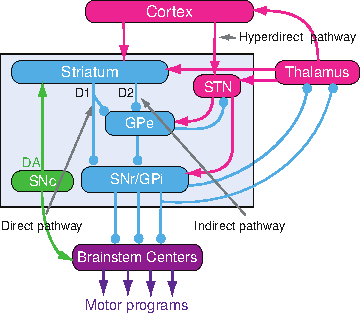
\includegraphics[width=0.7\linewidth]{ch-intro/figures/BGAnatomy}
		\caption[Anatomy of the Basal Ganglia]
		{\textbf{Schematic Anatomy of the basal ganglia.}
		The gray highlighted rectangle depicts the BG nuclei.
		Arrows show anatomical connections (\textit{red}: glutamatergic; \textit{blue}: GABAergic; \textit{green}: DAergic).
		STN:~subthalamic nucleus;
		GPe:~globus pallidus externus;
		SNc:~substantia nigra pars compacta;
		SNr:~substantia nigra pars reticulata;
		GPi:~globus pallidus internus;
		DA:~dopamine.
		Figure slightly modified from~\cite{Grillner2016BG}.
		}
		\label{fig:intro:BGAnatomy}
	\end{center}
\end{figure}

%=============================================================
\subsubsection{Striatum} \label{intro:anatomy:striatum}
%order of material: MSNs > interneurons > topography > DLS/DMS
The striatum is the main input nucleus of the \gls{bg} and one of the largest undivided structures in rodent brain atlas~\cite{Hintiryan2016NN,Hunnicutt2016}.
Despite having several cell types, GABAergic \glspl{msn} constitute~90--95\% of its neural population.
Their name stems from their morphological appearance, their size and the abundance of their dendritic processes~\cite{TURNER2000BasalFunction}.
\Glspl{msn} receive glutamatergic inputs from the entire cortex, thalamus, and amygdala.
These excitatory afferents make up 80\% of all the synapses in the striatum~\cite{Wilson2007GABAergicNeostriatum}.
Several other inputs modulate the responsiveness of the \glspl{msn} to massive excitatory synapses, namely \gls{da} afferents, inhibitory input from GABAergic interneurons (and from \gls{msn} collaterals), and input from cholinergic interneurons~\cite{Dudman2015Book}.
Consequently, \glspl{msn} are mostly quiescent, except during motor activity or in response to sensory stimuli~\cite{KandelBook2001}.
\par
Based on morphological and neurochemical identification, there are two major types of interneurons within the striatum, which make up~5--10\% of striatal neural population:
    the medium aspiny GABAergic interneurons, and the large aspiny cholinergic interneurons.
The most abundant type of GABAergic interneuron expresses parvalbumin.
Parvalbumin-positive interneurons are physiologically characterized by their hyperpolarized resting potential and fast spiking activity.
Thus, they are usually referred to as the \glspl{fsi}~\cite{Dudman2015Book}.
They target \glspl{msn} at the soma level by gap junctions and provide powerful GABAergic synapses to several hundreds of surrounding \glspl{msn}~\cite{Grillner2016BG, Gage2010FSI}.
Although they are scarce, with higher firing rate compared to \glspl{msn}, they are capable of delaying action potentials in the neighboring \glspl{msn}~\cite{Wilson2007GABAergicNeostriatum}.
\par
Large cholinergic interneurons are the other type of striatal interneurons.
Their soma could be as large as~40~$\mu$m in diameter, with expansive arborization and an axon that extends over~2~mm~\cite{Dudman2015Book}.
They have tonic discharge patterns, and in primate, are called \textit{tonically active neurons}.
\Glspl{fsi} and cholinergic interneurons are not noticeable in number, nonetheless, they are believed to strongly contribute to the dominance of inhibition in the striatum~\cite{Gage2010FSI}.
In addition to these two, several other types of interneurons within the striatum are described as well~\cite[see][]{Grillner2016BG, Dudman2015Book}.

\paragraph{Organization of Cortical Inputs}
It has been long known that corticostriatal projections are topographical, roughly following the rostro-caudal and latero-medial organization in the cerebral cortex.
For instance, frontal cortices project to rostral areas, sensorimotor cortex provides input to dorsal striatum, and parietal cortex to more caudal areas~\cite{Dudman2015Book}.
Such topographical organization suggests parallel circuits for limbic, cognitive, and sensorimotor processes via cortico-\gls{bg}-thalamo-cortical loops~\cite{Alexander1986}.
In this framework, the sensorimotor loop consists of \gls{dls}, ventrolateral thalamus, and sensorimotor cortices.
Similarly, the limbic (emotional) loop includes the ventral striatum, dorsomedial thalamus, and limbic areas (amygdala, limbic cortices, and hippocampus).
Finally, the cognitive (associative) loop comprise the \gls{dms}, anterior ventral thalamus, and frontal cortices~\cite{Jahanshahi2015NatRevNeurosci}.
However, reduced number of neurons from cortex to \gls{bg} outputs by a factor of more than one million, implies integration of information from different loops to shape the appropriate behavior~\cite{Boraud2018ProgNeurobiol}.
\par
In the dorsal striatum, loose somatotopic organization has also been long reported~\cite[see][as an early review]{Mink1996}.
In \citeyear{Carelli1991}, \citeauthor{Carelli1991} recorded from hundreds of neurons during movement and somatosensory stimulation.
They found that more than 70\% of recorded neurons in the \gls{dls} responded to movement, passive manipulation or cutaneous stimulation.
Moreover, neurons selective for an individual body part (e.g., forelimb, neck, snout,\dots) were generally located in close proximity, generating a somatotopic map~\cite{Carelli1991}.
Such an anatomical mapping from sensorimotor cortices to \gls{dls} has recently been quantitatively scrutinized in mice~\cite{Hunnicutt2016, Hintiryan2016NN}.
These studies, using multiple injections of anterograde tracers, constructed a comprehensive excitatory input map of the dorsal striatum.
\autoref{fig:intro:InputMap} shows an example of different cortical regions projecting to the \gls{dls} in a somatotopic manner.
Interestingly, cluster analysis of cortical regions projecting to arbitrarily-defined striatal voxels revealed dorsal striatal subregions which relatively agreed with parallel circuits for limbic, cognitive, and sensorimotor processes.
With the strictest clustering criteria, \citeauthor{Hunnicutt2016} identified two areas, which map roughly to the \gls{dls} and \gls{dms}\footnotemark~\cite{Hunnicutt2016}.
\footnotetext{
    \Gls{dls} and \gls{dms} correspond to the putamen and caudate nuclei, respectively.
    In primates, the internal capsule divides the striatum in two halves, thus the use of caudate-putamen nucleus instead of the striatum is more common.
    }
\begin{figure}[bth!]
  \begin{center}
    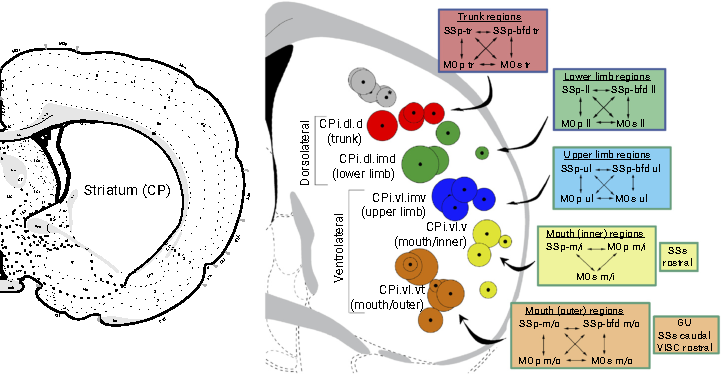
\includegraphics[width=0.9\linewidth]{ch-intro/figures/StriatumInputMap}
    \caption[Somatotopic map of cortical inputs to \gls{dls}]
    {\textbf{Somatotopic map of cortical inputs to \gls{dls}.}
    \textit{Left}: striatum in the rat brain atlas.
    \textit{Right}: input from somatosensory cortices form a topographic map in the \gls{dls}.
    Abbreviations are defined in the original reference and are not important for the purposes of this work.
    Figure adopted from~\cite{Hintiryan2016NN}.
    }
    \label{fig:intro:InputMap}
  \end{center}
\end{figure}
Of note, \gls{dms} and \gls{dls} have been suggested as functionally distinct areas as well, contributing to goal-directed and habitual behaviors, respectively~\cite{Yin2006NatRevNeurosci}.
Another noteworthy result concerns the extent of these areas.
The identified \gls{dls} receives inputs from motor cortex, somatosensory cortex, but also frontal association cortex, amygdala, and prelimbic cortex, and expands medially much larger than what has been traditionally regarded as \gls{dls}.
It has since been suggested that the sensorimotor information in the dorsal striatum is more prevalent than classically considered and it should be taken into account in studies concerning the function of the striatum~\cite{Robbe2018}.


\subsubsection{Direct/Indirect Pathways}
\label{intro:bg:pathways}
\Glspl{msn} are the majority of the neuronal population of the striatum.
They are homogeneously distributed in a way that the striatum lacks any architectural organization when all the neurons are stained in a histologic slice~\cite{Dudman2015Book}.
Nonetheless, \glspl{msn} are divided into two major categories, based on their neurochemistry and connectivity.
One class expresses \gls{d1} and projects directly to \gls{gpi}/\gls{snr} neurons, hence they form the so-called \emph{direct pathway}.
The second kind expresses \gls{d2} and projects to the \gls{gpe}.
This pathway, in turn, leads to the output nuclei through two routes:~monosynaptic~\gls{gpe}$\rightarrow$output, or bisynaptic~\gls{gpe}$\rightarrow$\gls{stn}$\rightarrow$output projections~\cite{TURNER2000BasalFunction}.
These \glspl{msn} form the \emph{indirect pathway}~(\autoref{fig:intro:BGAnatomy}).
\Gls{d1}-expressing neurons and \gls{d2}-expressing neurons exist in rather equal numbers and are intermingled and spread rather uniformly throughout the striatum~\cite{Dudman2015Book}.
The net effect of direct pathway activity is to inhibit the \gls{gpi}/\gls{snr}, thus releasing the target areas of the \gls{bg} from inhibition.
On the contrary, indirect pathway activity, through \gls{gpe} and \gls{stn}, disinhibits the output nuclei that in turn would cause further inhibition of \gls{bg} targets.
\par
\Gls{da} significantly modulates neuronal activity in the striatum.
\Gls{pd}, with many behavioral and cognitive ramifications, is characterized by degeneration of \gls{snc} neurons and \gls{da} depletion in the striatum~\cite[see][for a comprehensive review]{McGregor2019Neuron}.
Axons from \gls{snc} neurons arborize widely in the striatum.
They primarily synapse with principle neurons (\glspl{msn}), targeting the narrow necks connecting the spines to dendritic shafts, whereas cortical inputs mostly terminate on dendritic shafts.
This particular arrangement may be a mechanism by which \gls{da} release modulates cortical input to the \glspl{msn}~\cite{TURNER2000BasalFunction}.
This mechanism is of extra importance since \gls{d1}-expressing neurons are excited by \gls{da}, whereas \gls{d2} neurons are inhibited.
Thus \gls{da} signals can up-regulate or down-regulate the excitability of the direct and indirect pathways.



%============================================================
\subsection{Basal Ganglia as a Clock}
\label{ch:intro:BGTime}

Many brain structures have been proposed to contribute to time estimation.
Among them, the \gls{bg}, are especially of interest, since they are directly involved in motor processes as well~\cite{Grillner2015}.
Moreover, the \gls{bg} are also involved in reinforcement learning---selecting actions in an uncertain world in a way that maximizes reward in the long term~\cite{Petter2018}.
Such learning necessitates an understanding of temporal contingencies in order to maximize future rewards.
Behavioral data supports that animals build probabilistic models for timing of the reward and even adjust their models in response to modified reward delays~\cite{li2013PNAS}.
% In general, execution of any complex behavior requires proper timing of the comprising sub-actions.
\par
The \gls{bg} are often implicated in timescales of several hundreds of milliseconds to several seconds~\cite{Paton2018NeuronRev}.
Evidence of involvement of the \gls{bg} in timing stems from a variety of sources, including pathologies such as \gls{pd}, lesion studies, and pharmacological and genetic manipulations.
Following the taxonomy discussed in \autoref{ch:intro:taxonomy}, there is some evidence of involvement of the \gls{bg} in sensory timing.
\Citeauthor*{Rao2001} reported encoding of time intervals in the human striatum in a task in which subjects reported whether an interval were shorter or longer than a standard interval of 1200~ms.\footnotemark\
They also observed a dynamic network of cortical activity in inferior parietal, premotor, and dorsolateral prefrontal cortex.
These nodes in the network were attributed to different components of temporal processing, respectively, attention, memory, and interval comparison.
They ultimately concluded the implication of ``striatal dopaminergic neurotransmission in hypothetical internal timekeeping mechanisms"~\cite{Rao2001}.
\footnotetext{
    This paradigm is commonly referred to as ``interval categorization task".
    }
Moreover, \Citeauthor*{Pouthas2005} investigated interval categorization for two durations (450~ms and 1300~ms).
They observed ramping striatal activity during both intervals.
They concluded a direct role of the basal ganglia in duration estimation, and that the caudate nucleus ``may support a clock mechanism"~\cite{Pouthas2005}.
Similar evidence exists in other species as well.
\Citeauthor*{Gouvea2015Elife} trained rats in a sensory categorization task to judge whether an interval is shorter or longer than 1.5~s.
They decoded animals' choice and elapsed time from ensembles of striatal neuronal activity, whereas apparent behavior in an overhead video failed to do so.
Importantly, transient inactivation of the \gls{ds} impaired performance, however, it did not cause a systematic under-- or over--estimation~\cite{Gouvea2015Elife}.
\par
Furthermore, the \gls{bg} are also well studied for their role in motor timing.
\Citeauthor*{Matell2003} trained rats to receive a reward in a fixed interval reinforcement schedule.\footnotemark\
The interval alternated between 10~s (25\% of trials) and 40~s (75\% of trials).
After learning, animals increased their lever press rate around the reinforced intervals.
Electrophysiological recordings from the striatum showed neurons with tuned firing rate only around 10~s interval, but not 40~s, while apparent behavior of the animals is similar.
The authors then suggest that a population of duration-coding cells, each tune to different values, could accurately represent the elapsed time~\cite{Matell2003}.
\footnotetext{
    In operant conditioning, fixed interval reinforcement schedule refers to a type of conditioning whereby a response is reinforced only if a certain period of time has elapsed.
    }
\Citeauthor*{Mello2015} also used a similar task for intervals ranging between 12~s to 60~s.
They found striatal cells that rescaled their activity when intervals changed.
As rats adjusted to the new interval, time estimations decoded form population dynamics predicted animals' timing performance.
In another study, \Citeauthor*{Bakhurin2017JNeuro} used an operant conditioning paradigm in which the conditioned stimulus was followed by a delayed reward delivery (2.5~s after cue onset) and they monitored anticipatory licking of mice as behavioral readout of temporal perception.
After training, they started licking~$\sim$1.5~s after the conditioned stimulus.
Simultaneously recorded neurons in the striatum and orbitofrontal cortex displayed sequential activity during the interval.
A machine learning algorithm was then trained to decode the elapsed time from the stimulus onset.
They showed that both striatal and cortical networks ``encoded time, but the striatal network outperformed the orbitofrontal cortex".
Interestingly, removing the neurons modulated by licking activity from the decoder significantly reduced its performance, however, it still remained higher than chance level~\cite{Bakhurin2017JNeuro}.
\par
Another source of impact in the \glsentrylong{bg} is the neuromodulatory effect of \gls{da}.
\Glsentrylong{da}'s role in reward processing and circuit dynamics of the striatum is discussed in \autoref{intro:BGAnatomy} and \autoref{intro:BGMotor}.
\Gls{da} is also believed to be involved in timing~\cite{Paton2018NeuronRev}.
In a peak interval procedure\footnotemark, \Citeauthor*{DeCorte2019} found that \gls{d2} blockade delayed start and stop times for an interval of 6~s.
Whereas, blockade of \glspl{d1} delayed stop times only.
Then they stressed the role of the \gls{ds} in timing, with \gls{da} ``being particularly critical for the temporal control of action"~\cite{DeCorte2019}.
\footnotetext{
    Peak interval procedure is a common task used to study timing.
    Similar to fixed interval schedules, a cue indicates that a response will be reinforced only after a certain period of time has elapsed.
    The profile of the response around the interval is then studied.
    }
\Glsentrylong{da} neurons encode reward prediction errors which requires accurate reward predictions~\cite[see][]{Berke2018NN}.
\Citeauthor*{Takahashi2016} recorded from \gls{da} neurons of rats while they performed a task with uncertainty in reward timing and reward number.
Neuronal activity showed error signals in response to both types of prediction error, however, after ventral striatal lesions, neurons only responded to changes in reward number, and not reward timing.
These results suggested that time-dependant component of reward prediction of \gls{da} neurons might rely on the ventral striatum~\cite{Takahashi2016}.
In an interesting study, \Citeauthor*{Paton2016Sci} measured and manipulated the activity of \gls{da} neurons in a 1.5~s interval categorization task.
\Gls{da}ergic activity predicted animal's time estimates.
Transient activation/inhibition of \gls{da} neurons caused under--/over--estimation of the interval.
Hence, they concluded that ``\gls{da} neurons, which are so central to reward processing, exert control over time estimation"~\cite{Paton2016Sci}, although these results reflect \gls{da} function in general, not specifically in the \gls{bg}.
Similar to scaling of spiking activity in the striatum~\cite{Mello2015}, \gls{da} concentration in the \gls{ds} is also scalable to time intervals in several second time range~\cite{Howard2017}.
However, \citeauthor{Howard2017} then conducted a series of experiments and concluded that the \gls{da} signal in the \gls{ds} does not reflect interval timing per~se, rather it is specific to behavioral choice of action~\cite{Howard2017}.
\par
Deficits in temporal perception occur in many disorders.
Since pathologies usually affect multiple brain structures or manifest in several behavioral domains, it is unclear whether timing deficits are responsible for dysfunctions, or they are merely the result of other malfunctioning systems.
Schizophrenia, for example, is a complex psychiatric disorder with a wide range of symptoms, including: delusions, hallucinations, speech poverty, and timing deficits.
This impairment is reported in sensory and motor timing tasks and is associated with increased \gls{da} levels in the striatum, as well as abnormal activity in the dorsolateral prefrontal cortex and \gls{sma}~\cite[see][]{Snowden2019}.
Furthermore, it has been reported that individuals with attention deficit/hyperactivity disorder do not benefit from temporal predictabilities in an oculomotor task that displayed a target after a random delay~\cite{Dankner2017}.
Additionally, timing deficiency has also been reported in \gls{hd}.
Patients demonstrated lower sensitivity to temporal regularities and overall, poorer performance in different types of sensory timing tasks.
Their performance negatively correlated with the progression of the \gls{hd}~\cite{Cope2014}.
Finally, \gls{pd} also affects timing performance.
Lower timing performance has been reported in multiple tasks.
\Citeauthor*{Harrington1998} showed that \gls{pd} patients were impaired in sensory timing, in which `duration perception' was weaker compared to the control group.
Also, in a motor task, whereby subjects performed finger-tapping synchronized with a series of tones (in the subsecond range), \gls{pd} participants were significantly more variable~\cite{Harrington1998}.
Interestingly, it has been proposed that frequent exposure temporally-structured tones might alleviate motor symptoms of the \gls{pd}, especially gait and stride length~\cite{Dalla2017}.

%============================================================
\subsection{Basal Ganglia as a Cost Machine}
\label{intro:BGMotor}
\epigraph{Why do we and other animals have brains?\dots You may reason that we have one to perceive the world or to think, and that is completely wrong\dots We have a brain for one reason and one reason only, and that is to produce adaptable and complex movements.}
{\textit{Daniel Wolpert, TED talk}}
\noindent

Regardless of whether one agrees with Daniel Wolpert's strong words above, importance of volitional movement is trivial.
Control of movements has been associated with \gls{bg} for a long time.
This link dates back to the first descriptions of the behavioral deficits of \gls{pd} by James Parkinson in 1817.
% \Gls{pd} is characterized by loss of \gls{snc} neurons and their ascending projections to the striatum.
Tetriakoff, in 1919, performed postmortem analysis of the brains of patients diagnosed with \gls{pd} and first reported loss of dark-pigmented nigral neurons.
Ever since, motor dysfunctions of \gls{pd} are believed to be due to \gls{da} depletion in the striatum~\cite{Hornykiewicz2006,McGregor2019Neuron,Redgrave2010}.
\par
Three behavioral deficits are typical for \gls{pd} (although symptoms differ from patient to patient):
    1)~resting tremor, which is the most apparent;
    2)~rigidity and stiffness of muscles;
    3)~bradykinesia---reduced movement vigor.
Reduced vigor in \gls{pd} has been investigated to distinguish between speed-accuracy trade-off and energetic cost as two possible determinants of movement speed.
\Citeauthor{Mazzoni2007} asked \gls{pd} patients and age-matched control subjects to make self-paced arm movements as accurate as possible toward a target with a speed within the requested range~\cite{Mazzoni2007}.
After 20 successful trials, the required speed range and/or target distance changed to the next experimental condition.
Both groups of subjects, across all conditions (3~target distances, 4~speed ranges) achieved similar peak velocities and maintained the same level of accuracy.
However, patients needed significantly more trials to reach the criterion to advance to the next condition.
Analysis of those extra trials performed by the \gls{pd} patients demonstrated that they used a higher proportion of slower movements while retaining the speed range the same as control subjects.
Moreover, authors showed that the number of trials required to reach the criterion, as a measure of task difficulty, strongly correlated with subjects' average acceleration.
This linear contribution (denoted as $S_N$) was steeper for control subjects.
In other words, for any given difficulty of the task, \gls{pd} patients \textit{chose} a lower level of acceleration.
Similar linear relationship existed between number of trials to criterion and accuracy as well, but it was the same for control subjects and patient.
Thus, lower $S_N$ in \gls{pd} is not caused by a different speed-accuracy trade-off, rather another component of task difficulty related to the acceleration.
Authors then argue that acceleration also represents movement energy cost, and that \gls{pd} patients are more sensitive to energy expenditure.
These results suggest that \gls{snc} innervation of the striatum carries a `motor motivation' signal and lack thereof in \gls{pd} leads to a propensity for slow movements~\cite{Mazzoni2007}.
\par
Available methods in animal research provide an opportunity to further dissect the \gls{bg} circuits.
For instance, infusion of the GABA$_A$ agonist, muscimol, transiently inactivates the surrounding neurons, allowing the researcher to study the functional relevance of the targeted structure.\footnotemark
\Citeauthor{Desmurget2010JNeurosci} took advantage of this technique to acutely inactivate the sensorimotor territory of the \gls{gpi} in monkeys~\cite{Desmurget2010JNeurosci}.
The monkeys were trained to move a cursor using a joystick to a peripheral target and then it back to its original position.
Two experimental conditions differ in the degree to which successive target positions were predictable:
    random positioning of the target in each trial;
    or a fix sequence of four target positions.
\Gls{gpi} inactivation after overlearning the sequence did not prevent its execution, thus failing to support a role for the \gls{bg} in ``storage or execution of well learned motor habits".
The main impairment observed post-injection was reduced movement speed and amplitude in both conditions, i.e., random sequences and the overlearned sequence.
Thus, they conclude that the motor circuit of the \gls{bg} contributes to the kinematics of motor execution but not its production nor storage of learned sequences~\cite{Desmurget2010JNeurosci}.
\footnotetext{
    This technical approach is not free from skepticism.
    \Citeauthor{Otchy2015Nature} present convincing evidence that acute circuit manipulations, such as inactivation, have unintended consequences.
    In a complex dynamical system such as the brain, by transiently changing the activity of the area of interest, off-target down-stream structures are driven into a unnatural state that could have behavioral implications of its own~\cite{Otchy2015Nature}.
    }
Similar results have been reported from patients with pallidal and striatopallidal lesions.
They can generate normal grip force when explicitly instructed, however once left to their own, they fail to squeeze harder to earn more monetary compensation~\cite{Schmidt2008Brain}.
In general, reduced vigor in common in conditions of abnormal \gls{bg} function~\cite{}.
Importantly, in many of those tasks, including the two mentioned above, reduced vigor could also be the consequence of overestimation of the cost.




% 1- vigor reduction is very common
% 2- in most tasks, vigor reduction translates to energetic conservatism
\section[Motivation, Question and More]{Motivation, Question and the Organization of the Thesis}
\label{intro:question}

The work presented in this thesis has two fronts that might seem unrelated at first glance, but in this chapter I tried to present them on a conceptual continuum.
The first part is concerned with the question of how animals often act as though they have a sense of time.
Enormous body of experimental and theoretical research implicates plenty of brain areas as providers of a time signal.
Although such an internal mechanism could be affected by external factors (e.g., reward rate and motivation), however it is usually assumed to be the means by which well-timed actions are generated.
This is what I referred to as ``internal time estimation'', not that the world exterior to the brain is irrelevant, but meaning that the brain has a sense of time on its own that underlies behavior.
This mechanism is appealingly simple, predictive of many behavioral phenomena, and backed by neurophysiological data.
Alternatively, we hypothesized that there is no sense of time per~se, and that time is perceived through interactions with the environment.
In other words, the duration of an interval is displaced by its sensorimotor content.
Since movement generation is among the most basic functions of the nervous system and inevitably, it takes a certain duration to execute any action, elapsed time could just be inferred from actions (or similarly, sensory processes).
Such an ``embodied time estimation'' provides a much more parsimonious explanation, and is in alignment with the long-reported and replicated observation across many species that animals produce stereotyped motor sequences under temporal constraints.
Nonetheless, this hypothesis has not been very popular!
Perhaps partly due to technological limitations to monitor a wide range of animal behavior (in rodents, from locomotion to whisking and sniffing), especially in standard experimental paradigms inside Skinner boxes; and in my opinion, partly due to a general brain-centric view where the brain is the puppeteer of the body.
\par
To test the embodied timing hypothesis, we used a novel behavioral paradigm developed by~\citeauthor{Rueda2015NN}~\cite{Rueda2015NN} that is a powered treadmill with a reward contingent on timing of appetitive approaches (details are discussed in \autoref{ch:methods:methods}).
This task allows monitoring the location of the animals and kinematics of their locomotion.
Powered treadmill enabled us to manipulate dynamics of the environment in order to facilitate or hinder exploitation of the stereotyped motor sequences that we hypothesized are essential for solving the task.
We assumed if timing was internally-driven, animals should be able to perform the task without resorting to the stereotyped motor strategies.
Results from these experiments are presented in \autoref{ch:time}.
\par
The second facet of this work deals with the problem of implementation, i.e., how the brain generates the motor 
sequence it presumably uses to keep track of time.
Classic models of the \gls{bg} implicate the \gls{dms} in early phases of learning, and the \gls{dls} in executing the learned sequences, or controlling their kinematics.
Results from an earlier work in our group suggest that the overall behavior of the animals following transient inactivation of the \gls{dls} remains intact, although more variable~\cite{Rueda2015NN}.
Therefore, in this work, using a similar approach, we aimed to specify the function of the striatum in development and execution of this behavior.
In particular, we evaluated the role of the striatum, the main input to the \gls{bg}, in learning and controlling the kinematics of a motor sequence, by permanently lesioning its subareas (details are discussed in \autoref{ch:methods:tech}) in both na\"{i}ve and trained animals.
Results from these experiments are presented in \autoref{ch:lesion}.
\par
Finally in \autoref{ch:discussion}, I synthesize an overview of my Ph.D.\ project and discuss its meaning and implications.
Moreover, some possible shortcomings and directions for future works are laid out.
It also should be noted that I tried to write each chapter such that it would make sense on its own, regardless of the rest of the manuscript.
\glsresetall
\chapter{Methods} 
\label{ch:methods:methods}
Time perception is convoluted with motor functions.
As discussed in the \hyperref[ch:intro:intro]{first chapter}, disentangling the two has proven to be difficult, and often, overlooked.
Therefore, interpretations might have been biased toward disregarding the actual behavioral algorithms, in favor of the neuronal correlations.
Here, using a novel behavioral paradigm allowed studying the motor activity of the animals --and the function of the \gls{ds}-- as well as their timing performance.
In this chapter, I will discuss the behavioral task in detail, along with all the experimental and analytical methods used in this project.

\section{Experimental Tools} \label{ch:methods:exp}
In this section, all the conditions used in the time-estimation experiments and other experimental methods are described.

\subsection{Subjects}
Subjects were male Long-Evans rats.
They were 12 weeks old at the beginning of the experiments, housed in groups of 4 rats in temperature-controlled ventilated racks and kept under 12~h--12~h light/dark cycle.
All the experiments were performed during the light cycle.
Food was available \textit{ad libitum} in their homecage.
Rats had access to water for 30~min after every experimental session, while their body weights were regularly measured.
No animal was excluded from further analysis.
All experimental procedures were conducted in accordance with standard ethical guidelines (European Communities Directive 86/60 - EEC) and were approved by the relevant national ethics committee (Minist\`{e}re de l'enseignement sup\'{e}rieur et de la recherche, France).

\subsection{Task Apparatus}
Four identical treadmills were used for the experiments.
Each treadmill was placed inside a ventilated sound-attenuating box (\Autoref{fig:methods:taskRules}{a}).
Treadmills were 90~cm long and 14~cm wide, surrounded by plexiglass walls such that the animals were completely confined on top of the treadmill belt.
Treadmill belt covered the entire floor surface and was driven by a brushless digital motor (BGB 44 SI, Dunkermotoren).
A reward delivery port (solenoid valve) was installed on the front (relative to the turning direction of the belt) wall of the treadmill and released a $\sim$80~$\mu$L drop of 10\% sucrose water solution in case of a full reward.
An infrared beam was placed 10~cm from the reward port.
The first interruption of the beam was registered as \gls{et}.
A loudspeaker, placed outside the treadmill, was used to play an auditory noise (1.5~kHz, 65~db) to signal error trials.
Two strips of LED lights were mounted on the ceiling along the treadmill to provide visible and infrared lighting during trials and intertrials, respectively.
The animals' position was tracked via an overhead camera (Basler scout, 25~fps).
A custom-made algorithm detected the white coating of the rats and recorded its centroid as animals' position.
The entire setup was fully automated by a custom-made program (LabVIEW, National Instruments).
Experimenter was never present in the behavioral laboratory during the experiments.
\begin{SCfigure}%[bt!]
    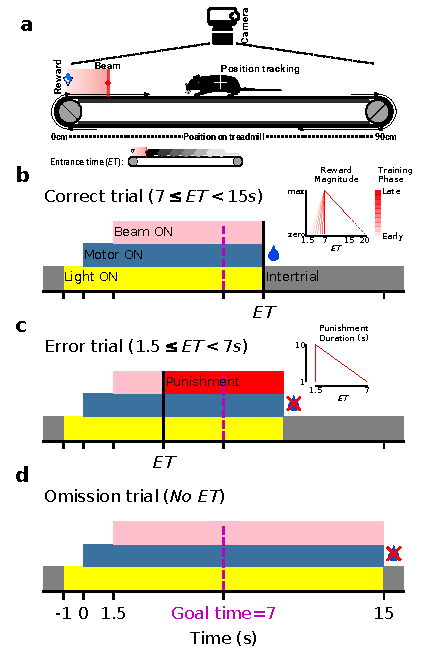
\includegraphics[scale=1]{ch-methods/figures/TaskRulesFULL.pdf}
    \caption[Treadmill Task Rules]
        {\textbf{Treadmill task and trial types.}
        \textbf{a)}
        Rats were enclosed on a powered treadmill.
        The infrared beam marked the reward area (red shaded area).
        During each trial, the belt pushed the animals away from the reward area and the first infrared beam interruption defined the \gls{et}.
        During trials and intertrials, the animal's position was tracked via a overhead video camera.
        \textbf{b)}
        Schematic description of a rewarded correct trial.
            \textit{Inset}: the magnitude of the delivered reward dropped linearly as \gls{et} increased (maximum reward at \acrlong{gt}).
            In early stages of training, smaller rewards were delivered for trials with ET~$<$~7~s.
            The smallest \gls{et} value that triggered reward delivery was progressively raised during learning.
        \textbf{c)}
        Schematic description of an error trial.
        Early \gls{et} triggered an extra running penalty and an audio noise.
            \textit{Inset}: the duration of the penalty was 10~s for the shortest \glspl{et} and fell linearly to 1~s for \glspl{et} approaching 7~s.
        \textbf{d)}
        Schematic description of an omission trial (no beam crossing between 1.5~s and 15~s).
        \textbf{b-d)}
        Note that \glspl{et} started to be detected 1.5~s after the motor start.
    }
    \label{fig:methods:taskRules}
\end{SCfigure}

\subsection{Habituation} \label{ch:methods:habituation}
Animals were handled 30~min per day for 3 days, then habituated to the treadmill for 3 to 5 daily sessions of 30~min, while the treadmill's motor remained turned off and a drop of reward was delivered every minute.
Habituation sessions resulted in systematic consumption of the reward upon delivery.

\subsection{Treadmill Task} \label{ch:methods:normalTrdTask}
Training started after handling and habituation sessions.
Each animal was trained once a day, 5 times a week (no training on weekends).
Each of the daily sessions lasted for 55~min and contained $\sim$130 trials.
Each trial started by turning the treadmill motor on at a fixed speed of 10~cm/s.
One second before motor onset, the ambient light was turned on (to warn the animals of the imminence of the belt movement).
The conveyor belt moved toward the rear of the treadmill (\Autoref{fig:methods:taskRules}{a}).
Three types of trials were defined based on the time the animal first interrupted the infrared beam, i.e., the \gls{et}, relative to the \gls{gt}.
Trials in which animals entered the reward area after the \gls{gt} were classified as \emph{correct} ($7\leq ET<15$, \Autoref{fig:methods:taskRules}{b}).
Trials in which animals entered the reward area before the \gls{gt} were classified as \emph{error} ($1.5\leq ET<7$, \Autoref{fig:methods:taskRules}{c}).
In case no infrared beam interruptions were registered in 15~s, the trial ended and was classified as \emph{omission} (\Autoref{fig:methods:taskRules}{d}).
The infrared beam was inactive during the first 1.5~s ($ET<1.5$) to give the opportunity to the animals to leave (passively or actively) the reward area at the beginning of each trial.
Additionally, the exact value of the \gls{et} determined a reward/punishment ratio.
The reward was a drop of sucrose solution and the punishment was a period of extra running.
The running penalty started when the animals erroneously crossed the infrared detector before \gls{gt} (error trial) and its duration varied between 10~s and 1~s, according to the error magnitude (\Autoref{fig:methods:taskRules}{c, inset}).
Thus, to maximize reward collection and minimize running time, animals should cross the infrared beam just after the \gls{gt}.

\subsubsection{Reward Profile} \label{ch:methods:reward}
The magnitude of the reward was a function of the \gls{et} and animal's performance in previous sessions.
Reward was maximal at $ET=GT$ and dropped linearly to a minimum (i.e., $\sim 38\%$ of the maximum) for \glspl{et} approaching 15~s (maximum trial duration).
Moreover, in the beginning of the training, partial reward was also delivered for error trials with $ET>ET_0$, where $ET_0$ denotes the minimum threshold for getting a reward.
The magnitude of this additional reward increased linearly from zero for $ET=ET_0$, to its maximum volume for $ET=GT$.
In the first session of training, $ET_0=1.5$~s and for every following session, it was updated to the maximum value of median \glspl{et} of the past sessions.
Once $ET_0$ reached the \gls{gt}, it was not updated anymore (late training reward profile in \Autoref{fig:methods:taskRules}{b, inset}).

\subsection{Alternative Task Conditions}
In addition to the ``normal'' treadmill task described above, several modified versions of the task were also designed to investigate the embodiment hypothesis.
In each of these conditions, a specific parameter of the task was altered, allowing us to study its effect on animals' performance.

\subsubsection{Variable Speed Condition}
In this condition, for each trial, treadmill speed was pseudo-randomly drawn from a uniform distribution between 5 and 30~cm/s.
During any given trial, the speed remained constant.
We used 5~cm/s as the lowest treadmill speed, because lower speeds generated choppy movements of the conveyor belt.
Also, velocities higher than 30~cm/s were not used, to avoid any physical harm to the animals.

\subsubsection{No-timeout Condition}
In the control condition, the infrared beam was not active during the first 1.5~s of the trials.
This \emph{timeout} period was sufficient to let the animals be carried out of the reward area by the treadmill, provided they did not move forward.
In the ``no-timeout'' condition, the infrared beam was activated as soon as the trial started.
Thus, in this condition, error trials corresponded to \glspl{et} between 0 and 7~s.
Consequently, animals were penalized if they were in the reward area when the trial started (i.e., $ET=0$~s).

\subsubsection{Short Goal Time Condition}
In this condition, the \gls{gt} was set to 3.5~s, half the value for the control condition.
The reward profile in this condition followed the same rules as for the control condition, except that reward was maximal at $ET=GT=3.5$~s.
Two different groups of animals were trained in this condition, one with treadmill speed set to the normal value of 10~cm/s, and another with treadmill running twice as fast.
In the short goal time condition, we also examined if the increased variability in \gls{et} could be attenuated when the penalty associated with early \gls{et} was increased and when reward magnitude was decreased for late \glspl{et}.
This was implemented by doubling the treadmill speed during the penalty period (from 10~cm/s to 20~cm/s), and the reward was delivered for a narrower window of \glspl{et} (maximal reward at $ET=GT=3.5$~s, and no reward after $ET=4.5$~s).
For proper comparison, we also examined the behavior of rats trained with $GT=7$~s when the running penalty was increased and the reward was decreased for late \glspl{et} (maximal reward at $ET=GT=7$~s, and no reward after $ET=9$~s).

\subsubsection{Immobile Condition}
In this condition, the treadmill motor was never turned on.
The ambient light was turned on during the trials and turned off during the intertrials.
Error trials were penalized by an audio noise and extended exposure to the ambient light.


\subsection{Reverse Treadmill Task} \label{ch:methods:rev}
This task differed from the normal treadmill task (\autoref{ch:methods:normalTrdTask}) in three critical properties:
\begin{itemize}[noitemsep]
    \item the treadmill moving direction was reversed, i.e., the conveyor belt moved toward the reward port;
    \item the treadmill speed was set at 8~cm/s (instead of 10~cm/s) to ensure that starting the trial in the back and remaining still (an reverse routine trial) would be rewarded, i.e., $ET\geq 7$.
    \item the intertrial duration was 20~s, instead of 15~s, to allow sufficient time for the animals to move to the back of the treadmill while the motor was still off.
\end{itemize}


\subsection{Locomotion Task} \label{ch:methods:loco}
A group of animals with a striatal lesion ($n=7$ DLS, $n=2$ DMS, and $n=3$ DS), and another group of non-lesioned animals ($n=12$) were used in this test to assess their general locomotor abilities.
Prior to this task, animals had full access to water and food for at least 3 days.
Then, they were placed on an unfamiliar treadmill, with a different structure (slanted walls and covered reward port) compared to the treadmill in which they were trained, while their position was being recorded using a side-mounted high-speed camera (200~fps).
During the first 10~min, the ambient light was turned off and the treadmill remained immobile.
Their exploratory locomotor activity, i.e., how much they moved along the treadmill, during this period is presented in \Autoref{fig:lesion:motorOk}{A}.
Then, in a free running task, they ran in trials of 30~s while the treadmill speed progressively increased across trials (5 trials at 0~cm/s, 2 trials at 10~cm/s, 3 trials at 15~cm/s and 5 trials at 20, 25, 30, 35, and 40~cm/s, total of 30 trials, data shown in \Autoref{fig:lesion:motorOk}{B}).
Each trial was followed by an intertrial of similar duration, while the ambient light and the treadmill motor were turned off.
The running speed reported is the average running speed of animals during the trials of any given treadmill speed.
\section{Technical Tools} \label{ch:methods:tech}

\subsection{Striatal Lesion} \label{ch:method:lesion}
\begin{figure}[bth!]
	\begin{center}
		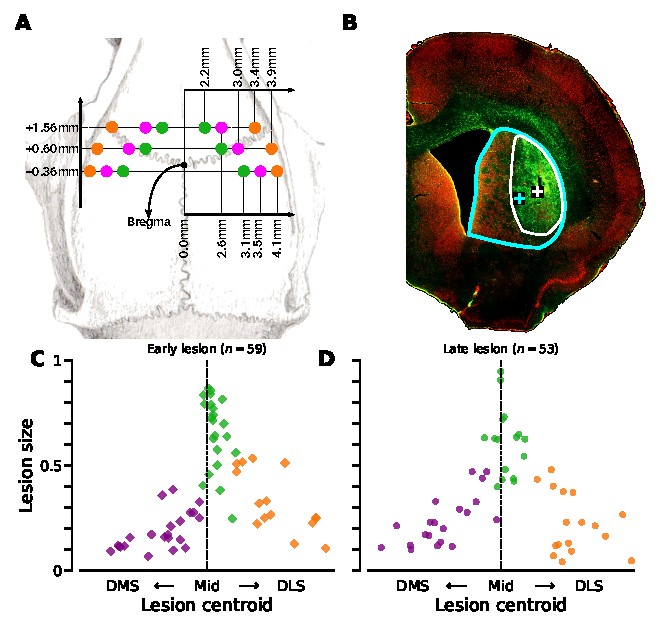
\includegraphics[scale=1]{ch-methods/figures/LesionSizeLocation.pdf}
		\caption
		{\textbf{Dorsal striatum lesion quantification.}
		\textbf{A)} Schematic of the lesion sites.
		\textbf{B)} Illustration of the quantification of the lesion size.
		For each coronal slide and hemi-striatum, the contour of the lesion was manually outlined using the GFAP staining.
		The relative size of the lesion (compared to the full striatum, manually outlined on the NeuN staining) and the coordinates of the lesion/striatum centroid was calculated.
		For each animal, the size and laterality were obtained by averaging data along the anteroposterior axis, for both left and right hemispheres.
		\textbf{C, D)} Lesion size versus laterality for animals that underwent lesion before (Early, \textbf{C}) and after (Late, \textbf{D}) extensive practice.
		Lesion quantification was performed blindly relative to behavioral analysis.
		In four animals with a striatal lesion performed after learning the task (late lesion), the lesion size quantification could not be properly performed.
		These animals were classified according to their injection coordinates in the surgery (3 DLS and 1 DMS), however they were excluded from any analysis that required the lesion size (hence the difference between the number of ``late lesion'' animals in this figure, $n=53$, and the total number of animals in \autoref{fig:lesion:task}, $n=57$).
		}
		\label{fig:method:LesionSizeLocation}
	\end{center}
\end{figure}
Anesthesia was induced with an intraperitoneal (IP) injection of a mixture of 100~mg/kg ketamine and 10~mg/kg xylazine and was maintained during the surgery with inhalant isoflurane gas (less than 3\%).
After shaving and cleaning the scalp, the animal was placed in the stereotaxic frame (Kopf instruments) and a local anesthetic (lidocaine) was injected under the scalp.
Then, an incision along the midline of the skull was made, followed by cleaning the exposed skull and drilling the craniotomies above the targeted areas.
To perform fiber-sparing lesion of the \gls{ds}, ibotenic acid (1\% in 0.1~M~NaOH, Fisher Scientific) was infused (Pump 11 Elite Nanomite, Harvard Apparatus, using a 10~$\mu$L WPI Nanofil syringe) in 6 specular sites bilaterally, at a rate of 90~nL/min.
The needle remained in place for 10~min following the injection to allow for the diffusion of the excitotoxic drug.
Then, the needle was retracted slowly to avoid backflow of the drug.
Once all the injections were performed, craniotomies were filled with bone wax, the skull was disinfected, and the skin was sutured.
Animals were allowed to recover for two weeks before resuming behavioral training.
After surgery, animals were housed alone for 3 days, to avoid getting hurt by the cagemates, and were force-fed if needed.
Injection coordinates (in~mm, with reference to Bregma, according to Paxinos) are shown in \Autoref{fig:method:LesionSizeLocation}{A} (each injection at $-5.6$~mm dorsoventral).
The infused volume in each site was 200~nL for DLS and DMS lesions, and 400~nL for \gls{ds} lesions.

\subsection{Immunohistochemistry}
At the end of the experiments, animals were euthanized with an overdose IP injection of $\sim$2~mL pentobarbital.
Then, they were perfused with 4\% paraformaldehyde and their brains were harvested for histological analysis of the lesion size and location.
Brains were coronally sliced on a vibratome at 60~$\mu$m thickness.
For each animal, six sections spanning the \gls{ds} along the rostrocaudal axis were selected (usually the following slice numbers: 5, 15, 25, 35, 45, and 55 for consistency) and submerged in 0.1~M~PBS.
Then, PBS was replaced with citrate buffer (10~mM) for 10~min at room temperature.
Next, slices were submerged with a blocking solution, consisting of PBS with 0.3\% triton and 15\% normal goat serum (NGS) for 120~min at room temperature.
Then, the solution was replaced with another consisting of 2~$\mu$L anti-NeuN antibody (Merks Millipore, MAB377) and 0.5~$\mu$L of anti-GFAP antibody (Agilent, Z033429-2) diluted in 200~$\mu$L of the blocking solution, kept overnight at 4~$^{\circ}$C.
Sections were then rinsed twice in PBS, 10~min each, at room temperature, before being submerged again in 1~$\mu$L of donkey anti-mouse antibody (Al555, red), 1~$\mu$L of donkey anti-rabbit antibody (AL488, green) diluted in 400~$\mu$L of PBS for 120~min at room temperature.
Finally, they were washed twice in PBS, for 10~min each time, and mounted for microscopy.

\subsection{Lesion Quantification}
Whole slices were imaged using an Apotome microscope (Zeiss, 28126), and stitched together in the processing software (Zeiss Zen).
Then for each slice, the ventricule, the striatum, and the lesioned area were manually outlined (\Autoref{fig:method:LesionSizeLocation}{B}) bilaterally in the image processing software (ImageJ, Fiji).
The size and the centroid coordinates were automatically computed for all of the above-mentioned areas.
Next, the anteroposterior location of each slice was also approximated according to the rat brain atlas (Paxinos).
\par
The lesion size reported in this paper is the ratio of the lesion volume over the volume of the striatum.
Both regions of interest (lesion and striatum) were approximated as a truncated cone between any two consecutive sections, and the volume was accordingly calculated and summed up.
\Autoref{fig:method:LesionSizeLocation}{C-D} show the lesion coordinates of all the animals trained in the normal treadmill task.
The type of the lesion (\gls{dls}, \gls{dms} or \gls{ds}) was determined visually and confirmed by comparing the centroid location of the lesion to that of the entire striatum.
Animals with a \gls{dls} lesion in one hemisphere and a \gls{dms} in another ($n=7$) were excluded from this manuscript.
Four rat brains were imaged improperly, they are automatically removed from any analysis that required the lesion size.


\subsection{Statistics}
All statistical comparisons were performed using resampling methods (permutation test and bootstrapping).
These non-parametric methods alleviate many concerns in traditional statistical hypothesis tests, such as distribution assumptions (e.g., normality assumption under analysis of variance), error inflation due to multiple comparisons, and sensitivity to unbalanced group size.
\par
We used the permutation test to compare the performance of two groups of animals during training on a session-by-session basis, such as in \Autoref{fig:time:varTrd}{b}, and \Autoref{fig:lesion:EarlyLesionLearning}{A}.
To simplify the description~\cite[see][for the complete description]{Fujisawa2008NN}, let's assume, as in \Autoref{fig:time:varTrd}{b}, we have ${\mathbf{X}=[X_1, X_2,...,X_n]}$, where $X_i$ is the set of \glspl{et} of all the animals in session~$i$.
Similarly, we have $\mathbf{Y}$ that contains \glspl{et} from another experimental condition.
Here, the null hypothesis states that the assignment of each data point in $X_i$ and $Y_i$ to either $\mathbf{X}$ or $\mathbf{Y}$ is random, hence there is no difference between $\mathbf{X}$ and $\mathbf{Y}$.
\par
In short, the test statistic was defined as the difference between smoothed (using Gaussian kernel with $\sigma =0.05$) average of $\mathbf{X}$ and $\mathbf{Y}$ for each session~$i$: $D_0(i)$.
I then generated one set of surrogate data by assigning \gls{et} of each animal in session $i$ to either $X_i$ or $Y_i$, randomly.
For each set of surrogate data, the test statistic was similarly calculated, i.e.,~$D_m(i)$.
This process was repeated 10,000 times for all the statistical comparisons in this manuscript, obtaining: $D_1(i),\ldots,D_{10000}(i)$.
\par
At this step, two-tailed pointwise p-values could be directly calculated for each $i$, from the $D_m(i)$ quantiles~\cite{Fujisawa2008NN}.
Moreover, to compensate for the issue of multiple comparisons, we defined global bands of significant differences along the session index dimension.
From 10,000 sets of surrogate data, a band of the largest $\alpha$-percentile was constructed, such that less than 5\% of $D_m(i)$s broke the band at any given session $i$.
This band (denoted as the \textit{global band}) represents the threshold for significance, and any break-point by $D_0(i)$ at any $i$ is a point of significant difference between $\mathbf{X}$ and $\mathbf{Y}$.
\par
A similar permutation test was also used when comparing only two sets of \textit{unpaired} data points (such as in \Autoref{fig:time:shortSharp}{e}, comparing control vs. short~GT groups).
The same algorithm was employed, having only one value for index $i$.
If none of the $D_m(i)$s exceeded $D_0(i)$, the value $p<0.0001$ was reported (i.e., less than one chance in 10,000).
\par
For paired comparisons (such as in \Autoref{fig:time:varTrd}{f} and in \Autoref{fig:lesion:rev}{C}), I generated the bootstrap distribution of mean differences ($n=10000$ with replacement).
Significance was reported if 95\% confidence interval (CI) of the pairwise differences differed from zero (i.e., zero was not within the CI)~\cite{Efron1994}.
For example, in \Autoref{fig:time:varTrd}{f, right}, the 95\% CI of pairwise differences is $(19, 27)$.
Since this interval does not contain zero, it is reported significant, whereas in \Autoref{fig:time:shortSharp}{e}, the CI of the comparison between normal and sharp short~GT is $(-0.17, +0.01)$ which includes zero, and hence is reported non-significant.
\par
Exceptionally, for the comparison in \Autoref{fig:time:shortSharp}{h}, even though it is not paired, I used bootstrapping, because I did not have enough data points to perform the permutation test.
In this case, the resampled distribution ($n=10000$ with replacement) for each group was calculated, and it was reported significant, since the distributions did not overlap at 95\% CI.
\par
Finally, in \Autoref{fig:time:ImmTrd}{f}, I used repeated measures correlation implemented in the Pingouin package~\cite{PingouinToolbox}.
This technique relaxes the assumption of independent data points, since each animal contributes more than one to the analysis.
\section{Data Analysis} 
\label{ch:methods:dataAnalysis}

Data from each behavioral session was stored in separate text files, including position information, entrance times, treadmill speeds, and all the task parameters.
Position information was then smoothed (Gaussian kernel, $\sigma = 0.3$~s).
The entire data processing pipeline was implemented in python, using open-source libraries and custom-made scripts.
We used a series of Jupyter Notebooks to process, quantify, and visualize every aspect of behavior and to generate all the figures in this manuscript.
All the Jupyter Notebooks, as well as the raw data necessary for full replication of the figures (alongside other complementary information) is publicly available via the Open Science Foundation.
The links to the respective repositories could be found from~\cite{Safaie2020PNAS,JuradoParras2020}.

\paragraph{Motor Routine Definition}
A trial was considered \emph{routine}, if all the following three conditions were met:
\begin{itemize}[noitemsep]
    \item the animal started the trial in the front (initial position $< 30$~cm);
    \item the animal reached the rear portion of the treadmill during the trial (maximum trial position $>50$~cm);
    \item the animal completed the trial (i.e., it crossed the infrared beam).
\end{itemize}
Then, we quantified the percentage of trials in which animals performed the above motor routine in each session (such as in \Autoref{fig:lesion:task}{C}).

\paragraph{Speed Calculation}
Unless otherwise stated, speed in this manuscript refers to the velocity with which animals outran the treadmill toward the reward port.
For every trial, it was calculated based on the time the animal takes to run from 60~cm to 40~cm along the treadmill.
Speed for each training session is the average speed across its trials (\Autoref{fig:lesion:task}{J}).
Furthermore, in \Autoref{fig:lesion:maxPos}{B}, we categorized the animals based on whether they had an effect on their running speed after the striatal lesion (black), or not (gray).
Animals were assigned to the black group ($\Delta$Speed$<0$) if the average speed of 5 consecutive stable sessions after the lesion (i.e., session $+8$ to $+13$) were lower than that of 5 consecutive sessions before the surgery (i.e., sessions $-5$ to $-1$).


\paragraph{Reverse Routine Definition}
A trial was considered \emph{reverse routine} if the following conditions were met:
\begin{itemize}[noitemsep]
    \item the animal started the trial in the back of the treadmill (initial position $> 60$~cm);
    \item the animal completed the trial (i.e., it crossed the infrared beam).
\end{itemize}
Percentage of reverse routine trials is analogous to the percentage of routine trials, only in the reverse treadmill.


\paragraph{Definition of Frontal Trials}
Frontal trials are defined as trials in which the animal remained in the frontal portion of the treadmill (i.e., position $<30$~cm) for the entire first 5~s after trial onset.


\paragraph{Speed Modulation Analysis}
In \Autoref{fig:lesion:motorOk}{C-D}, we split the trajectories that strictly followed the wait-and-run routine (see the definition of the Max.\ Pos.) into trials with the maximum position between 40 and 60~cm (Mid) and those between 70 and 90~cm (Back).
The data was pooled from the last 5 sessions before (\Autoref{fig:lesion:motorOk}{D, left}) and after (\Autoref{fig:lesion:motorOk}{D, right}) the lesion.
To improve the reliability, animals were discarded if they did not have at least 10 trials in the Mid and 10 trials in the Back condition (trials that strictly followed the wait-and-run routine, their maximum position was within the range, and for which the speed could have been defined).
Fewer number of animals in the \Autoref{fig:lesion:motorOk}{D, left} panel was due to the fact that most animals performed the wait-and-run routine by going all the way to the rear portion of the treadmill, thus not enough Mid trials existed.


\paragraph{Definition of Max.\ Pos.}
The maximum position an animal reached along the treadmill before initiating the run bout toward the reward in the wait-and-run routine was quantified as Max.\ Pos.\ in \Autoref{fig:lesion:maxPos}{D}.
Therefore, Max.\ Pos.\ was only calculated for trials that strictly followed the wait-and-run routine, i.e., total immobility followed by continuous running until reaching the infrared beam.
A trial was qualified if the following conditions were met:
\begin{itemize}[noitemsep]
    \item the animal started the trial in the front (initial position $< 30$~cm);
    \item the animal moved at least 10~cm backward (maximum position $\geq 40$~cm);
    \item the animal remained still while being pushed backward by the treadmill (movements shorter than 0.1~s and slower than 5~cm/s were ignored to correct for jitter in position detection);
    \item the animal performed an uninterrupted running epoch (staying immobile or moving backward shorter than 0.1~s was ignored to correct for jitter in position detection);
    \item the animal completed the trial (i.e., it crossed the infrared beam).
\end{itemize}
Notice that compared to the definition of the routine trials, the threshold for maximum position in the second criterion is relaxed (40~cm, compared to 50~cm) to allow detection of trials with a reduced maximum position.
To increase the reliability, any session with fewer than 10 trials for which Max.\ Pos.\ could be defined was excluded from further analysis.
The reported value of Max.\ Pos.\ for each session is the average value across its trials (\Autoref{fig:lesion:maxPos}{D}).


\paragraph{Normalizing Speed and Max. Pos.}
In \Autoref{fig:lesion:maxPos}{B,~D}, to normalize each animal’s performance according to its own behavior prior to the lesion, behavioral measures (speed and Max. Pos.) of individual animals during the illustrated sessions were subtracted from the median value of the respective measure during the pre-lesion sessions.
Animals were included only if the behavioral measure could be defined in at least half of the illustrated sessions.
Different $n$ in panel~D compared to~B, and in panel~B compared to the total number of animals (\Autoref{fig:lesion:task}{H}) is due to this criterion.
\glsresetall
\chapter{Embodied Timing} \label{ch:time}

To investigate how animals adapt their behavior to temporal regularities in their environment, we challenged Long-Evans rats in a treadmill-based behavioral assay that required them to wait for 7~s before approaching a ``reward area''.\footnotemark
\footnotetext{
    The materials related to time experiments in this document were largely borrowed from~\cite{Safaie2020PNAS}.
}
The treadmill belt was surrounded by long walls.
The front wall was equipped with a device delivering rewards (a drop of sucrose solution) and an infrared beam, located 10~cm from this device, which defined the limit of the reward area (see \Autoref{fig:methods:taskRules}{a}).
Animals were first familiarized with the apparatus and were trained to lick drops of the sucrose solution delivered every minute while the treadmill was immobile (see \autoref{ch:methods:habituation} for more details).
Then, rats were trained once a day (Mondays to Fridays) for 55~minutes in the proper treadmill waiting task.
Each daily session contained $\sim$130 trials interleaved with resting periods of 15~s (intertrials, while motor was off).
Each trial started by turning the treadmill motor on at a fixed speed of 10~cm/s.
The conveyor belt moved toward the rear of the treadmill (\Autoref{fig:methods:taskRules}{a}).
The \gls{et} of the animals in the reward area (detected by the first interruption of the infrared beam in each trial) relative to a \emph{\gls{gt}} (7~s after motor onset) defined 3~types of trials:
    Trials in which animals entered the reward area after the \gls{gt} were classified as correct ($7\leq ET<15$, \Autoref{fig:methods:taskRules}{b});
    Trials in which animals entered the reward area before the \gls{gt} were classified as error ($1.5\leq ET<7$, \Autoref{fig:methods:taskRules}{c});
    Finally, if in 15~s an animal failed to interrupt the infrared beam, the trial ended and was classified as omission (\Autoref{fig:methods:taskRules}{d}).
Interruptions that occurred during the first 1.5~s ($ET<1.5$) were ignored (in other words, the infrared beam was not active during the first 1.5~s of trials) to allow the animals to leave (either passively or actively) the reward area at the beginning of each trial.
Moreover, the exact value of the \gls{et} determined the reward/punishment ratio (see \autoref{ch:methods:reward}).
A punishment period of extra running started when the animals erroneously crossed the infrared beam before the \gls{gt} ($1.5\leq ET<7$).
The punishment duration varied between 10~s and 1~s, according to the error magnitude (\Autoref{fig:methods:taskRules}{c, inset}).
In addition, to progressively encourage the animals to enter the reward area just after the \gls{gt}, the smallest \gls{et} value that triggered reward delivery was raised across sessions, according to each animal's performance, until it reached the \gls{gt} (\Autoref{fig:methods:taskRules}{b, inset} and see \autoref{ch:methods:reward} for details).
Thus, to maximize reward collection and minimize running time, animals should approach the reward just after the \gls{gt}.

\section{Treadmill Task}
\label{ch:time:treadmill}
During the first training sessions, animals started most trials in the front of the treadmill, mostly ran in the reward area and interrupted the infrared beam before the \gls{gt} (\Autoref{fig:time:CtrlTrd}{a, top, c, left}).
Progressively, across training sessions, animals waited longer and after $\sim$15 sessions, they reliably entered the reward area just after the \gls{gt} (\Autoref{fig:time:CtrlTrd}{b}).
Interestingly, for a large majority of animals, precisely waiting 7~s before entering the reward area was associated with the performance of a stereotyped motor sequence on the treadmill (\Autoref{fig:time:CtrlTrd}{a, bottom,~c, right}).
This motor sequence (or routine) consists of the following steps:
\begin{enumerate}[noitemsep, label=\Roman*.]
    \item Animals began each trial in the reward area, i.e., they stayed in the reward area during the intertrials;
    \item When the trial started, they remained largely still while being pushed away from the reward area until they reached the rear wall;
    \item After reaching the rear wall, they ran across the treadmill, without pause, and crossed the infrared beam.
\end{enumerate}
\begin{figure}[bt!]
    \begin{center}
      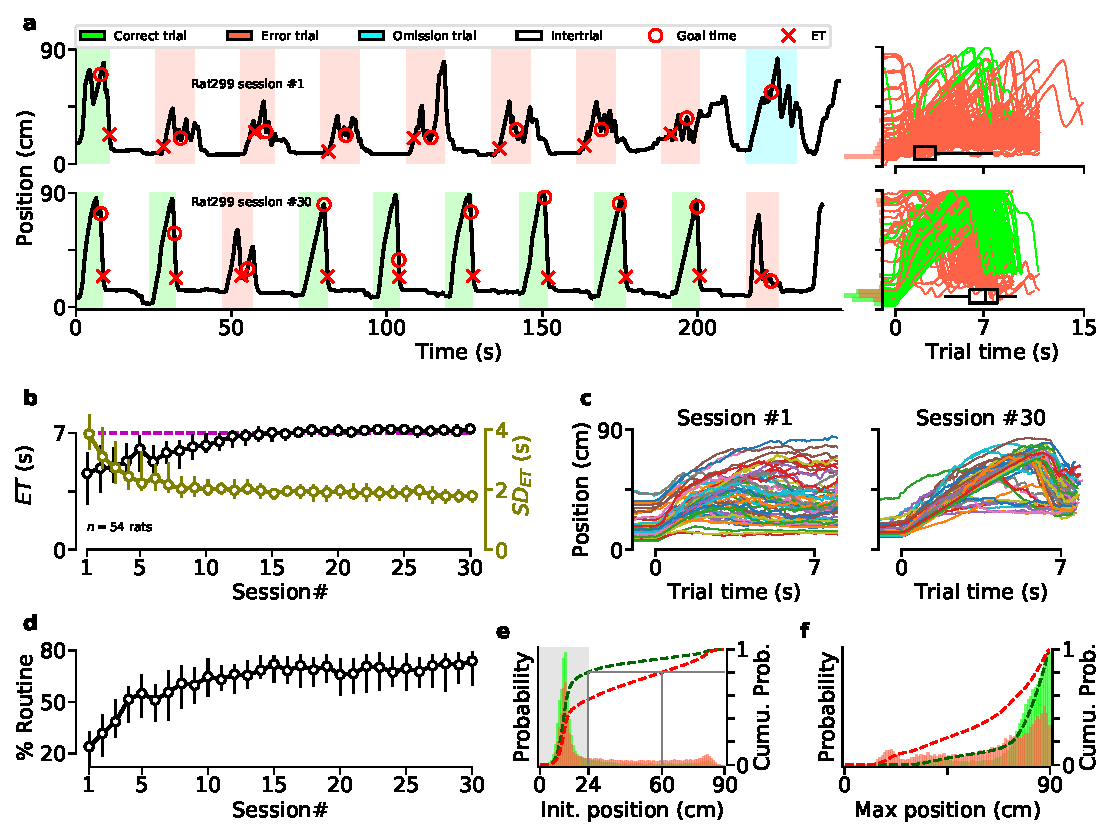
\includegraphics[width=.8\linewidth]{ch-time/figures/CtrlTrd.pdf}
      \caption[Control Condition]
      {\textbf{Most animals developed a unique stereotyped motor sequence.}
      \textbf{a)}
      \textit{Left}: illustration of an animal's trajectory on the treadmill during 9 consecutive trials of the 1st (\textit{top}) and 30th (\textit{bottom}) training sessions.
      On the y-axis, 0 and 90 indicate the treadmill's front (reward port) and rear wall, respectively.
      \textit{Right}: trajectories for all trials during the 1st (\textit{top}) and 30th (\textit{bottom}) sessions (same animal as in left panels).
      Distributions of initial positions for correct (green) and error (red) trials are shown on the y-axis.
      Black horizontal boxplots depict entrance time range (center line, median; box, 25th and 75th percentiles; whiskers, 5th and 95th percentiles).
      \textbf{b)}
      Median entrance time ($ET$) in the reward area for the first 30 daily training sessions.
      Circles indicate group median and error bars, the median range (25th and 75th percentiles) across animals for $ET$ and on the right y-axis,$SD$ of $ET$~($SD_{ET}$) values.
      The dashed magenta line shows the goal time (7~s).
      \textbf{c)}
      Median trajectory of all the trials for the 1st (\textit{left}) and 30th (\textit{right}) training sessions.
      Each line represents a single animal~($n=54$).
      \textbf{d)}
      Session-by-session percentage of trials during which animals performed the stereotyped front-back-front routine (see \nameref{ch:methods:methods}).
      Circles indicate group median and error bars, the median range across animals (25th and 75th percentiles).
      \textbf{e)}
      Probability distribution function~(PDF) of the position of the animals at the beginning of each correct (green) and error (red) trial, from sessions \#20 to \#30.
      Dashed lines represent cumulative distribution functions (right y-axis).
      The gray area indicates that in trained animals,~80\% of correct trials began with the animal located near the front of the treadmill.
      \textbf{f)}
      PDF of the maximum position along the treadmill reached by animals before crossing the beam~($=ET$).
      Only trials in which animals were initially located in the front of the treadmill (gray area in panel~e) were included.
    }
    \label{fig:time:CtrlTrd}
    \end{center}
  \end{figure}
The percentage of trials for which animals used this motor routine increased during learning (\Autoref{fig:time:CtrlTrd}{d}).
Even though a strong preference for the reward area was observed for both correct and error trials, the probability to start a trial in the front portion of the treadmill was higher for correct trials compared to error trials (\Autoref{fig:time:CtrlTrd}{e}), a tendency that developed progressively during training (\autoref{fig:appendix:initPos}).
\par
In addition, if an animal started a trial in the front portion of the treadmill, the probability of reaching the back of the treadmill was higher in correct trials than in error trials (\Autoref{fig:time:CtrlTrd}{f}), further confirming that correct trials were mostly those in which the animals followed the wait-and-run routine and effectively reached the back of the treadmill before running forward toward the reward area.
However, a significant fraction of the animals (14 out of 54) did not develop such a strategy (\Autoref{fig:time:CtrlTrd}{c, right}, and \Autoref{fig:appendix:BadCtrl}{a}).
Compared to these animals, those regularly following the wait-and-run routine entered the reward area later, demonstrated reduced variability, and an increased percentage of correct trials (\Autoref{fig:appendix:BadCtrl}{b-d}).
Note that one cannot exclude the possibility that animals categorized as \textit{other} in \autoref{fig:appendix:BadCtrl} also used a more subtle stereotyped motor routine not captured by tracking the average body position along the treadmill length.
Anyway, the above results suggest that following a front-back-front trajectory through the ``wait-and-run'' routine is the most reliable strategy to accurately respect the 7~s-rule of the task.


\section{Variable Speed Condition}
\label{ch:time:varSpeed}

It could be argued that task parameters (length of the treadmill, its speed, position of the infrared beam,\dots) favored the development of this stereotyped strategy.
Indeed, depending on the initial position of the animal body at trial onset, it can take up to~7 or~8 seconds for the animals to passively reach the back of the treadmill (\Autoref{fig:time:CtrlTrd}{a}) after which they can start running toward the reward area without the need to estimate time at all!
Thus, in the following experiments, we examined how accurately animals respected the \gls{gt}, when distinct task parameters were modified in a way that hampered the use of this simple wait-and-run motor routine.
First, we trained a new group of rats in a version of the task in which, for each trial, the speed of the treadmill was randomly selected from a uniform distribution between~5 and 30~cm/s (\Autoref{fig:time:varTrd}{a}).
\begin{figure}[bt!]
  \begin{center}
    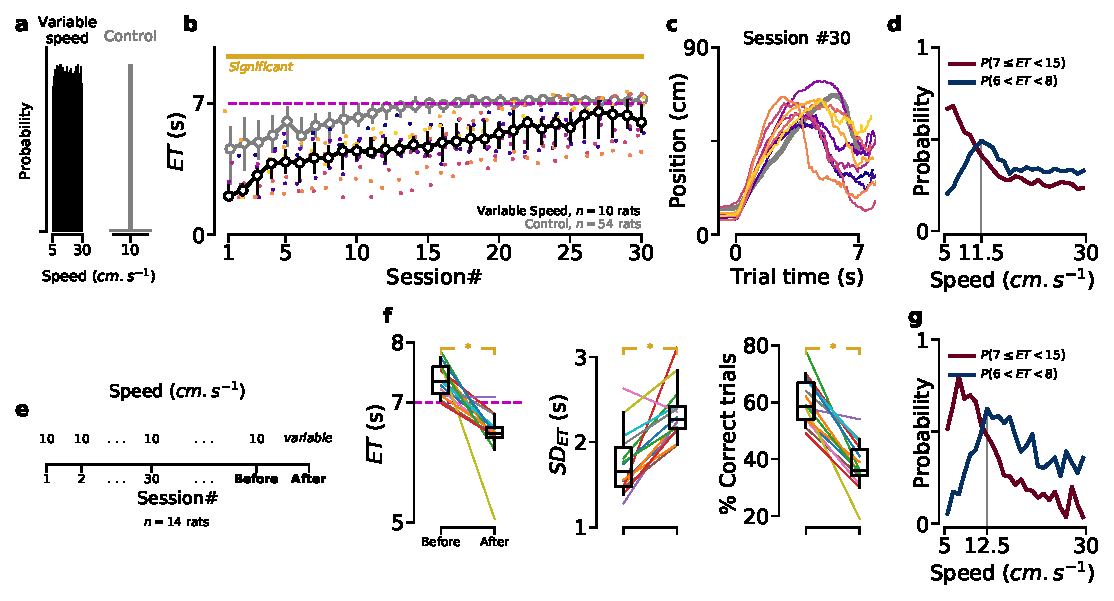
\includegraphics[width=\textwidth]{ch-time/figures/VarTrd.pdf}
    \caption[Variable Speed Condition]
    {\textbf{Decreased temporal accuracy when the treadmill speed randomly changed every trial.}
    \textbf{a)}
    For each trial, treadmill speed was either fixed at 10~cm/s (control condition, same data as in \autoref{fig:time:CtrlTrd}), or randomly selected from a uniform distribution between 5 and 30~cm/s (variable speed condition).
    \textbf{b)}
    Median \gls{et} for animals trained in the variable speed (black), and control (gray) conditions.
    Colored dots indicate individual ``variable speed'' animals.
    Golden line in this manuscript shows statistically significant differences between groups (permutation test).
    \textbf{c)}
    Median trajectory of variable speed animals in session \#30 (same colors as in panel~b).
    \textbf{d)}
    Probability of correct (7~$\leq$~ET~$<$~15~s) and precise (6~$<$~ET~$<$~8~s) trials, given the treadmill speed, for variable speed animals (session~\# $\geq$20).
    \textbf{e)}
    After extensive training in the control condition, some animals ($n=14$) were tested in a probe session with variable speed.
    \textbf{f)}
    Median \gls{et} (\textit{left}), $SD$ of ET (\textit{middle}), and percentage of correct trials (\textit{right}) in the sessions before and after the change in the speed condition.
    Each line represents a single animal.
    Asterisks indicate significant differences (non-parametric paired comparison).
    \textbf{g)}
    Similar to panel~d, for the data collected from the probe session.
  }
  \label{fig:time:varTrd}
  \end{center}
\end{figure}
We found that, during the course of training, these animals consistently failed to wait as long as the animals trained in the control version of the task (`control' group, \Autoref{fig:time:varTrd}{b}).
Still, the average trajectories of animals extensively trained in this ``variable speed'' condition revealed that they followed a front-back-front trajectory (\Autoref{fig:time:varTrd}{c}).
Accordingly, the probability of performing a correct trial, given different speeds, fell rapidly from~5 to~$\sim$15~cm/s and was lowest for the fastest treadmill speeds (\Autoref{fig:time:varTrd}{d}).
Indeed, it shows that when the treadmill speed was fast, performing the wait-and-run strategy resulted in error trials, as animals reached the back region of the treadmill earlier, compared to when the treadmill speed was slow.
Interestingly, we also found that the probability of precise approaches, i.e., entering the reward area at the~\gls{gt}$\pm 1$~s sharply peaked for a treadmill speed (11.5~cm/s) that is suitable to perform the wait-and-run motor sequence (\Autoref{fig:time:varTrd}{d}, notice that this speed is very close to the speed in the control condition).
Finally, when rats extensively trained in the control version of the task underwent a single probe session with variable speed (\Autoref{fig:time:varTrd}{e}), all measures of performance dropped significantly (\Autoref{fig:time:varTrd}{f}).
Examining the probability of correct trials and precise approaches given the treadmill speed, resembled those of animals well-trained in the variable condition and suggested that rats kept performing the wait-and-run routine they previously learned in the control condition (compare \Autoref{fig:time:varTrd}{g} and \Autoref{fig:time:varTrd}{d}).


\section{No-Timeout Condition}
\label{ch:time:nto}

In the control condition,~$\sim$80\% of correct trials started while animals were in the reward area (\Autoref{fig:time:CtrlTrd}{e}).
If rats relied on an internal clock-based algorithm to accurately time their entrance in the reward area, they should adapt relatively easily to a perturbation in their initial starting position.
To test this prediction, we trained a group of rats in a modified version of the task that penalized starting the trials in the front region of the treadmill.
This was done by activating the infrared beam as soon as the motor was turned on, i.e., the trial start.
Opposite to the control condition that the infrared beam was initially inactive for a \emph{timeout} period that lasted~1.5~s after treadmill onset to allow the animals to be carried out of the reward area by the conveyor belt.
In this ``no-timeout'' condition, error trials corresponded to \glspl{et} occurring between 0 and 7~s after motor onset (\Autoref{fig:time:ntoTrd}{a}).
 \begin{figure}[bt!]
  \begin{center}
    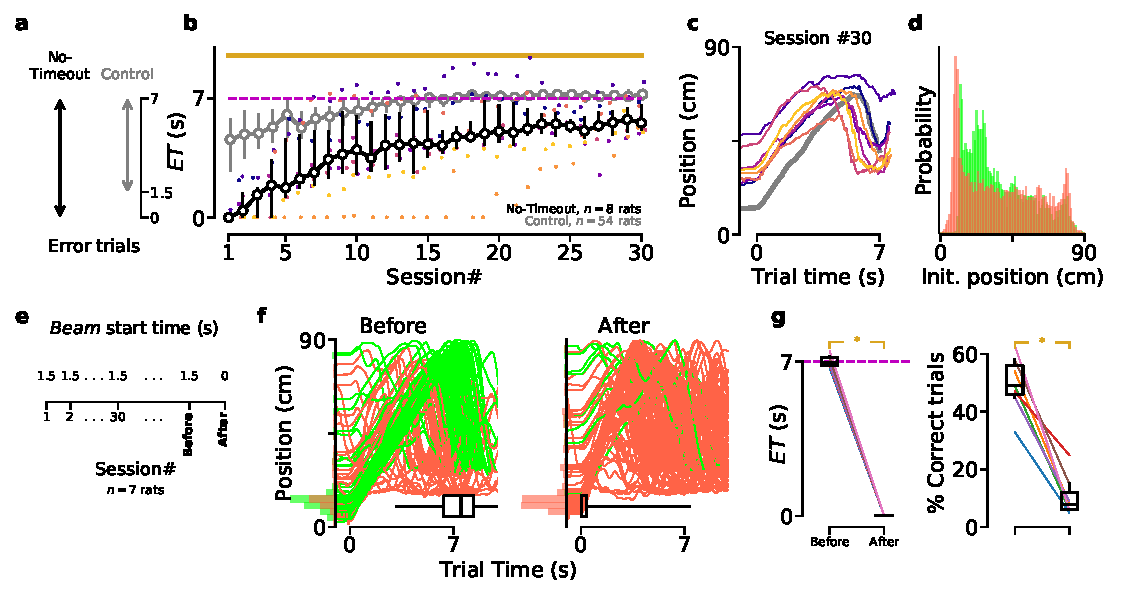
\includegraphics[width=.8\linewidth]{ch-time/figures/NToTrd.pdf}
    \caption[No-Timeout Condition]
    {\textbf{Decreased temporal accuracy when animals are penalized for starting trials in the reward area.}
    \textbf{a)}
    In the control condition, animals had a 1.5~s timeout period to leave the reward area after motor onset.
    In ``no-timeout'' condition, crossing the infrared beam any time before 7~s registers as an error trial.
    \textbf{b)}
    Median $ET$ for animals trained in the no-timeout (black), and control (gray) conditions.
    Colored dots indicate performance for individual no-timeout animals.
    \textbf{c)}
    Median trajectory of no-timeout animals (same colors as in panel~b) in session~\#30.
    \textbf{d)}
    PDF of the no-timeout animals' positions at the beginning of each trial, from sessions~\#20 to~\#30.
    \textbf{e)}
    After extensive training in control condition, animals ($n=7$) were tested in a no-timeout probe session, in which the beam started at the beginning of the trial, rather than 1.5~s later.
    \textbf{f)}
    Trajectories of a representative animal in the last control session (\textit{left}), and the probe session (\textit{right}).
    \textbf{g)}
    Median $ET$s (\textit{left}), and percentage of correct trials (\textit{right}) in the sessions immediately before and after the change in beam start time.
    Each line represents a single animal.
    Asterisks indicate significant differences (non-parametric paired comparison, see \autoref{ch:methods:tech}).
    }
    \label{fig:time:ntoTrd}
  \end{center}
\end{figure}

Animals trained in this condition never reached the level of timing accuracy displayed by animals in the control condition (\Autoref{fig:time:ntoTrd}{b}).
Still, no-timeout animals followed a front-back-front trajectory (\Autoref{fig:time:ntoTrd}{c}) and correct trials were associated with the animals starting the trials just behind the infrared beam (\Autoref{fig:time:ntoTrd}{d}).
The stereotyped reliance on the wait-and-run strategy was also demonstrated by the fact that rats extensively trained in the control condition kept performing the exact same trajectory when tested in a single probe session under the no-timeout condition, leading to many error trials and punishments (\Autoref{fig:time:ntoTrd}{e-g}).


\section[Short~GT \& Sharp Conditions]{Short Goal Time and Sharp Reward Conditions}
\label{ch:time:shortGT}

We next examined how animals behaved when the \gls{gt} was set to~3.5 seconds (\autoref{fig:time:shortSharp}), a condition in which the performance of the wait-and-run strategy would lead to late $ET$s (and smaller rewards, and more running time) because it can take up to~$\sim$8~s for the animals to passively travel from the front to the rear portion of the treadmill.
Animals successfully entered the reward area after~3.5~s and reduced their variability across training sessions (\Autoref{fig:time:shortSharp}{a}), but as a group, they demonstrated an elevated \gls{et} variability compared to animals trained in the control condition, with \gls{gt} set to 7~s (\Autoref{fig:time:shortSharp}{e}).
From the averaged trajectories of ``short~GT'' animals measured once their performance plateaued, it appeared that 3 subjects out 7 followed a front-back-front trajectory by running toward the rear portion of the treadmill.
\begin{figure}[!bt]
  \begin{center}
    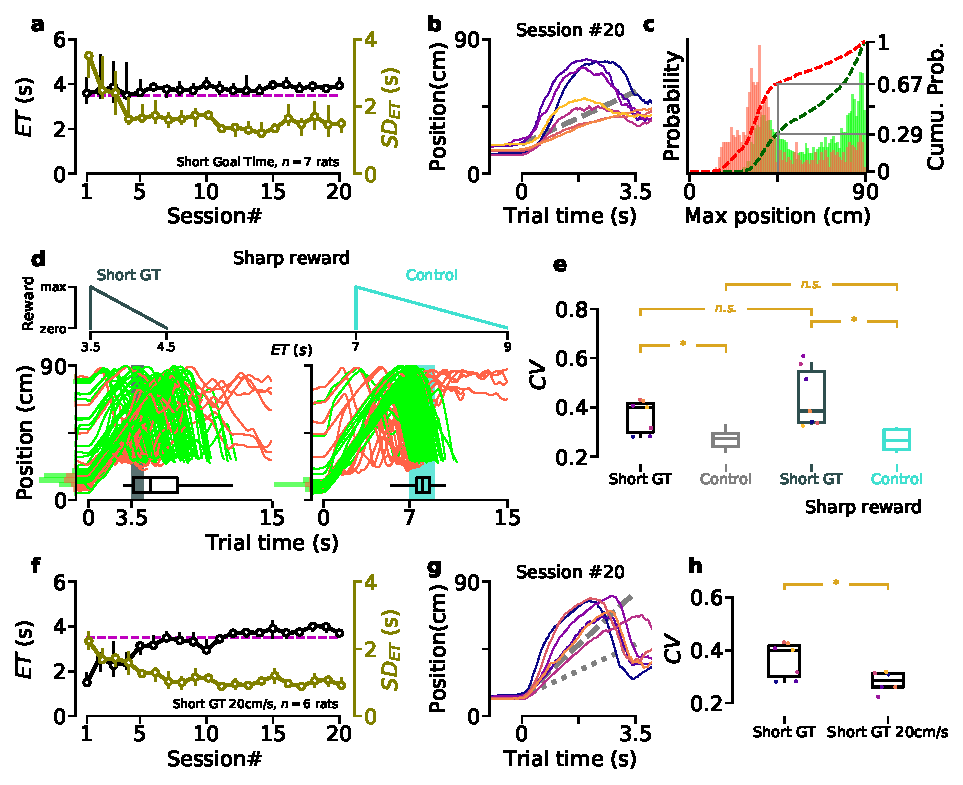
\includegraphics[width=\textwidth]{ch-time/figures/ShortGT-SharpTrd.pdf}
    \caption[Short~GT \& Sharp Conditions]
    {\textbf{Decreased temporal accuracy when the goal time is short.}
    \textbf{a)}
    Median $ET$ during training ($GT=3.5$~s).
    \textbf{b)}
    Median trajectory of ``short~GT'' animals after training.
    Colored lines indicate performance of individual animals.
    Dashed line's slope shows the treadmill speed (10~cm/s).
    \textbf{c)}
    PDF of the maximum position of the short~GT animals for correct (green) and error (red) trials.
    Dashed lines represent cumulative distributions (right y-axis).
    Data collected from session~\#~$\geq15$.
    \textbf{d)} 
    Sharp reward condition applied to short~GT and control experiments.
    \textit{Top}: reward profiles of the sharp reward condition applied to the short~GT (dark) and the control experiments (light).
    \textit{Bottom}: trajectories of 2 illustrative sessions after extensive training in sharp condition (\textit{left}, short~GT; \textit{right}, control).
    Highlighted areas indicate the reward window.
    \textbf{e)}
    Coefficient of variation~($CV$) for short~GT and control experiments with normal (the first two boxes), and sharp (the last two boxes) reward profiles.
    Data collected and averaged once performance plateaued.
    Short~GT vs. Control: $p<0.0001$;
    Sharp short~GT vs. Sharp control: $p<0.0001$.
    \textbf{f)}
    Similar to panel~a, for another group of animals trained to wait 3.5~s while the treadmill speed was 20~cm/s.
    \textbf{g)}
    Similar to panel~b, for animals of panel~f.
    Dashed line's slope shows the treadmill speed (20~cm/s).
    Dotted line's slope shows 10~cm/s.
    \textbf{h)}
    $CV$ for short~GT and short~GT at 20~cm/s conditions (same colors as in panels~b,~g).
    Data collected and averaged once performance plateaued.
    }
    \label{fig:time:shortSharp}
  \end{center}
\end{figure}
The other 4 animals remained still when the treadmill started and accelerated forward before reaching the rear wall (\Autoref{fig:time:shortSharp}{b}).
Interestingly, after training, in 67\% of the error trials, the rats started running forward before reaching even the middle of the treadmill (\Autoref{fig:time:shortSharp}{c}, compared to the red histogram in \Autoref{fig:time:CtrlTrd}{f}).
Conversely, after initiating a trial in the reward area, the probability of visiting a deeper portion of the treadmill was much stronger in correct than error trials, reinforcing the idea that accurate timing was accomplished by exploiting the most salient physical features of the environment, i.e., touching the rear wall (\Autoref{fig:time:shortSharp}{c}).
Accordingly, the 3 rats that followed the front-back-front trajectory by running toward the back were less variable than those that passively stayed still before running toward the reward area from the middle of the treadmill (\Autoref{fig:time:shortSharp}{e}, same color code as in panel~b).
In addition, among animals trained in the short goal time condition, we found that the magnitude of the backward displacement on the treadmill was negatively correlated with \gls{et} variability ($r=-0.49, p=2.7\times 10^{-3}$, Pearson's correlation).
\par
In the short~GT condition, animals became proficient more rapidly than in the control condition (compare \Autoref{fig:time:shortSharp}{a} with \Autoref{fig:time:CtrlTrd}{c}).
However, their variability remained similar, which is why short~GT animals have a higher coefficient of variation (\Autoref{fig:time:shortSharp}{e}).
The increased \gls{et} variability when the \gls{gt} is 3.5~s may be explained by the fact that the task is generally easier in this condition and that animals do not need to be very precise.
To test this possibility, we increased the punishment for error trials and decreased the reward size for late \glspl{et}.
In this ``sharp reward'' condition, the performance of the animals trained with the short~GT was even more variable, while animals trained in the control experiment managed to adapt and perform with similar accuracy (\Autoref{fig:time:shortSharp}{d-e}).
This result confirms that under short~GT condition animals can not accurately time their entrance in the reward area, even when exposed to harsher punishments.
\par
Finally, another group of animals was trained with \gls{gt} set to 3.5~s and treadmill speed set to 20~cm/s (i.e., twice as fast as in the control condition).
This experiment once again provided the animals with an \textit{easy} wait-and-run motor strategy that would result in \glspl{et} close to the \gls{gt} (\Autoref{fig:time:shortSharp}{f}).
Expectedly, after treadmill start, these animals stayed immobile until reaching the end of the treadmill, utilizing the aforementioned strategy, similar to the animals trained in the control condition (\Autoref{fig:time:shortSharp}{g}).
Higher treadmill speeds usually should be regarded as less comfortable, nonetheless these animals displayed reduced \gls{et} variability compared to the animals trained at 10~cm/s (\Autoref{fig:time:shortSharp}{h}).


\section[Immobile Condition]{Immobile Treadmill Condition}
\label{ch:time:immobile}

The above results suggest that, in a task requiring animals to produce a motor response according to a fixed temporal constraint, the possibility to perform a stereotypical motor sequence adapted to salient features of the environment (here, taking advantage of the full treadmill length and its physical boundaries) critically determines temporal accuracy.
However, it could still be argued that by starting the treadmill motor and moving the animals in a certain direction, we are \textit{priming} them to develop a stereotyped motor response.
Although the short~GT condition was designed to remedy that, it still had a moving belt.
To further de-bias our approach, we trained a group of animals in a version of the task in which the treadmill never started (trial onset was signaled by switching the ambient light on).
In this condition, animals displayed a strong impairment in respecting the \gls{gt}, compared to animals trained in the control condition, to the degree that a few of the animals did not show signs of learning even after extensive training (\Autoref{fig:time:ImmTrd}{a,~b}).
\begin{figure}[bt!]
  \begin{center}
    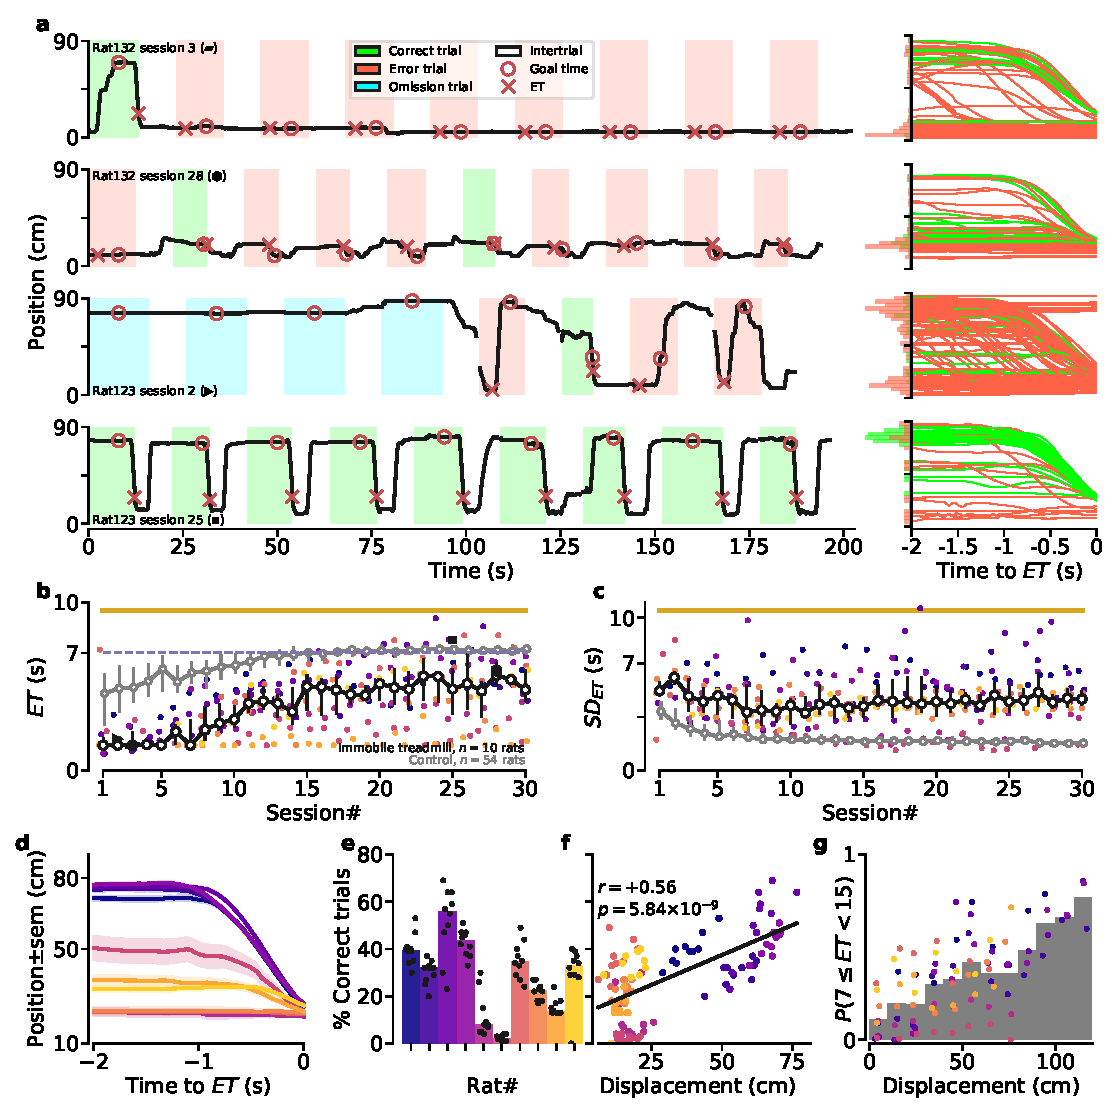
\includegraphics[width=.8\linewidth]{ch-time/figures/ImmTrd.pdf}
    \caption[Immobile treadmill]
    {\textbf{Performance of animals trained while the treadmill remained immobile.}
    \textbf{a)}
    \textit{Left}: illustrations of the positions of two animals on the immobile treadmill for~9 consecutive trials, early (\textit{1st row:}~Rat~\#132-session~\#3, \textit{3rd row:} Rat~\#123-session~\#2) and late (\textit{2nd row:} Rat~\#132-session~\#28, \textit{4th row:} Rat~\#123-session~\#25) during training.
    \textit{Right}: trajectories for all the trials of the corresponding sessions on the left, aligned to the $ET$.
    Distributions of positions 2~s before $ET$, for correct (green) and error (red) trials are shown on the y-axis.
    \textbf{b)}
    Median $ET$ across sessions for "immobile treadmill" animals.
    Filled black markers correspond to the sessions illustrated in panel~a.
    \textbf{c)}
    Similar to panel~b, for the standard deviation of entrance times ($SD_{ET}$).
    \textbf{d)}
    Median trajectory aligned to $ET$ of each "immobile treadmill" animal (only correct trials from sessions~\#20 to~\#30 are considered; shaded regions denote standard error).
    \textbf{e)}
    Median percentage of correct trials for each immobile treadmill animal (same sessions as in panel~d).
    Each dot represents one session.
    \textbf{f)}
    Repeated measures correlation between the percentage of correct trials and average displacement during a session.
    Each dot represents one session.
    \textbf{g)}
    PDF of a correct trial, given the displacement of an animal.
    Each dot represents the average probability for an individual animal, during a single session.
    \textbf{(e-g)}
    Analyses based on the same sessions as in panel~d.
    Individual animal color code is preserved in panels~b-g.
    }
    \label{fig:time:ImmTrd}
  \end{center}
\end{figure}

On average, animals entered the reward area later and later across sessions, but displayed a constant high variability in \gls{et} (\Autoref{fig:time:ImmTrd}{c}), as opposed to learning in the control condition that is accompanied by both increasing \glspl{et} and falling variability (\Autoref{fig:time:CtrlTrd}{b}).
Interestingly, we noticed that correct trials preferentially occurred when animals crossed the treadmill from the rear wall to the reward area, as evident in \Autoref{fig:time:ImmTrd}{a,~d,~e}.
Moreover, after extensive training, a robust correlation was observed between the percentage of correct trials and displacement of the animal on the treadmill (\Autoref{fig:time:ImmTrd}{f}).
In other words, more locomotor activity was associated with better timing performance.
In a related analysis, we showed that the probability of a correct trial given different displacement values is an ascending function (\Autoref{fig:time:ImmTrd}{g}).
For example, chances of doing a correct trial without much displacement (i.e., $\leq 10$~cm) are $\sim$0.1, while the three rats that performed trials with over 100~cm displacement on the treadmill, succeeded almost 80\% of the time.
\par
Lastly, animals well-trained in the immobile treadmill condition during several weeks were then challenged in the control condition (i.e., by simply setting the treadmill speed at 10~cm/s).
These animals improved their behavior at the same pace and with the same wait-and-run routine as na\"ive animals (\Autoref{fig:appendix:Imm2Ctrl}{a-c}).
Thus, animals that previously learned to wait in one version of the task did not learn faster than na\"ive animals when challenged in a second version of the task with distinct movement requirement but an identical time constraint, once again demonstrating that task proficiency relied primarily on the acquisition of a motor sequence rather than an abstract knowledge of time.
\glsresetall
\chapter{Striatum and Effort} \label{ch:lesion}
In the last chapter, I presented many experiments, all in support of the hypothesis that time estimation is embodied and that accurate timing requires stereotyped interaction with the environment.
Stereotyped interactions appear as motor routines to the external observer, e.g., the superstitious behavior of pigeons (\autoref{ch:intro:EmbodiedClock}) and the wait-and-run routine of rats (\autoref{ch:time}).
Thus, the question of how the brain measures the elapsed time is translated to how the brain generates or controls motor routines.
In this study, we focused on the striatum, the main input nuclei of the \gls{bg}, since its motor-related functions are long-reported, well-known, and still debated.\footnotemark\
We took advantage of the motor routine developed by the animals in the treadmill task, i.e., the wait-and-run motor routine (\Autoref{fig:time:CtrlTrd}{d}) to investigate the role of the striatum in performing and controlling the kinematics of motor routines.

\footnotetext{
    The materials related to striatal function in this document were largely borrowed from~\cite{JuradoParras2020}.
}
To obtain a drop of sweetened water, rats had to wait for a fixed \gls{gt} of 7~s from trial onset before entering the reward area located at the front of the treadmill, while the belt was slowly moving backward (\Autoref{fig:lesion:task}{A}).
Across training sessions composed of $\sim$120~trials, animals learned to wait longer and longer to enter the reward are just after the \gls{gt} and achieve higher percentage of correct trials (\Autoref{fig:lesion:task}{B}, and \autoref{fig:appendix:CorrectTrialCurve}).
Task proficiency was clearly associated with the acquisition and reliable performance of the following routine (\Autoref{fig:lesion:task}{C}):
\begin{enumerate}[noitemsep]
    \item during the intertrial, following the consumption of the reward, rats remained in the reward area;
    \item when the treadmill was turned on (trial onset), they did not move and let the belt carry them away from the reward area;
    \item when they reached the rear wall of the treadmill, they started outrunning the treadmill to reenter the reward area, i.e., the \gls{et} just after 7~s ($ET\geq GT$).
\end{enumerate}
After 2--3 weeks of daily practice, rats used this wait-and-run routine in about 75\% of the trials (\Autoref{fig:lesion:task}{C}, see \autoref{ch:methods:dataAnalysis} for the operational definition of this routine).
Finally, learning this routine was paralleled by a robust invigoration of the running phase of the motor routine toward the reward area (\Autoref{fig:lesion:task}{D}).

\section{Striatal Lesion}
\label{ch:lesion:lesion}
\begin{figure}[bth!]
 \begin{center}
	\makebox[\textwidth][c]{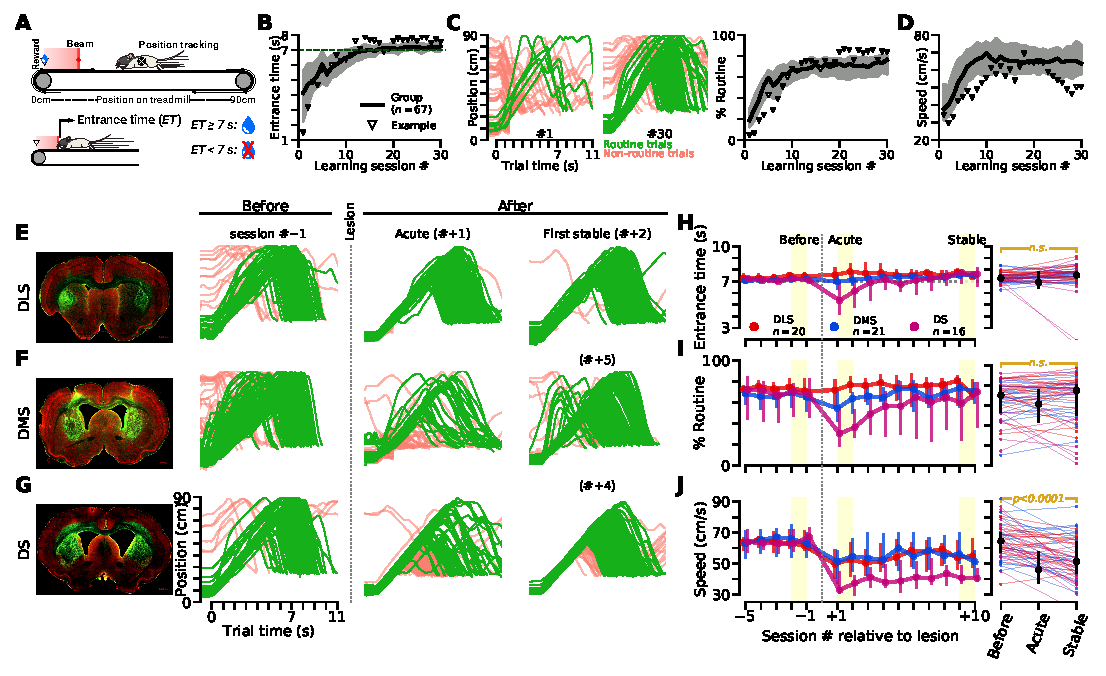
\includegraphics[scale=1]{ch-lesion/figures/Task_Example_Group.pdf}}
	\caption[The Striatum Energizes Motor Routines]
	{\textbf{The striatum is necessary to energize the running component of a motor routine.}
	\textbf{(A)} Experimental apparatus and task rules.
	\textbf{(B-D)} Performance across training sessions and animals.
	Shaded areas represent the 2nd and 3rd quartiles. Triangles represent the changes in performance of an example animal. 
	All the trajectories of this animal during sessions \#1 and \#30 are shown in C (left). 
	\textbf{(E-G)} Histology (1st column, GFAP in green shows gliosis, red is Neun) and trajectories from single animals with bilateral lesions of the dorsolateral, dorsomedial and dorsal striatum (E: DLS, F: DMS: G: DS).
	\# indicates session number relative to lesion break.
	\textbf{(H-J)} Left, Session-by-session time course of the lesion effect on ET (H), percentage of routine usage (I) and speed when animals run toward the reward area (I).
	Right, group data statistical comparison before vs after lesion (10,000 permutations).
	}
	\label{fig:lesion:task}
 \end{center}
\end{figure}
\par
Once the performance was stable, after at least 30 training sessions, we performed fiber-sparing lesions of the striatum ($n=57$ animals, for the lesion protocol, see \autoref{ch:method:lesion}).
The lesions targeted either the \gls{dls} or the \gls{dms}, or both territories, the entire \gls{ds} (\Autoref{fig:lesion:task}{E-G}, see also \autoref{fig:method:LesionSizeLocation}).
Behavioral testing resumed two weeks after the lesion surgery.
Visually, the animals had normal behavior (locomotion, food/water intake) in their homecage at the end of the recovery period.
\par
After the lesion, the behavior of the animals could be divided into an `acute' phase in the first few sessions post-lesion, and a `stable' phase that begins $\sim$9 sessions after the lesion and persists.
This dichotomy does not apply to every animal, apparently animals with bigger lesions have a stronger acute effect.
This can be seen in example animals of \Autoref{fig:lesion:task}{F,~G}, and at the population level in \Autoref{fig:lesion:task}{H}, however, the case illustrated in \Autoref{fig:lesion:task}{E} is an example of a rat with smaller lesion and no acute condition.
To better visualize the acute effect, I grouped the first two post-lesion sessions and presented their average statistics throughout this manuscript.
Similarly, sessions $+9$ and $+10$ were also grouped to represent the stable effect of the lesion.
Animals with this acute effect ran toward the reward area prematurely after trial onset and, consequently, a drop in the usage of the wait-and-run routine was observed during these first post-lesion sessions (\Autoref{fig:lesion:task}{I}).
Surprisingly, most of these animals recovered from this initial impairment and after a few additional sessions, task proficiency was similar to the pre-lesion level (\Autoref{fig:lesion:task}{H-I}, right panels, compare the stable condition to the `before' condition).
Moreover, for most of the animals with a lesion restricted to the DLS and DMS, task proficiency was virtually unaltered when resuming behavioral testing.
We then looked at animals' speed, the velocity with which they outran the opposing treadmill in the third step of the wait-and-run motor routine (see \autoref{ch:methods:dataAnalysis} for the definition).
Strikingly, the animals' speed was irreversibly reduced following striatal lesion (\Autoref{fig:lesion:task}{I}).
In addition, the difference in speed due to lesion was strongly correlated with the size of the lesion (\Autoref{fig:appendix:spd}{A}).
\begin{figure}[tb!]
    \begin{center}
        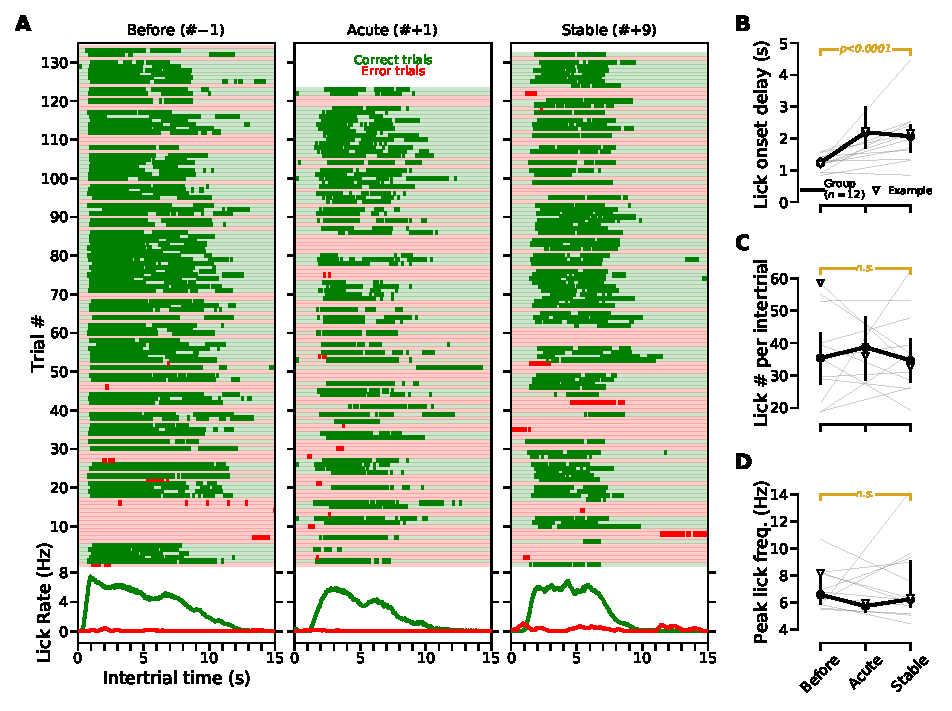
\includegraphics[width=\textwidth]{ch-lesion/figures/Lick.pdf}
        \caption[Licking Behavior After Striatal Lesion]
        {\textbf{Licking behavior mostly unaffected by the striatal lesion.}
        \textbf{A)}
        Trial-by-trial licking pattern (\textit{top}) and averaged lick rate aligned to intertrial onset for a single animal in 3~sessions (1~just before and 2~after lesion).
        Each tick shows one lick in the reward delivery port.
        \textbf{B-D)}
        Effect of striatal lesion on lick onset delay (\textit{B}), number of licks per intertrial (\textit{C}) and peak licking frequency (\textit{D}).
        Same color code for individual lesion type as in \autoref{fig:lesion:task}.
        }
        \label{fig:lesion:lick}
    \end{center}
\end{figure}
Moreover, the maintained task proficiency following striatal lesion suggested that the motivation of the animals to perform the task and to obtain rewards was preserved.
In agreement with this statement, animals with a striatal lesion kept licking the reward after committing correct trials(\Autoref{fig:lesion:lick}{A}).
They licked the number of times after reward delivery and also their peak lick frequency was not affected (\Autoref{fig:lesion:lick}{C-D}).
However, they systematically started to lick later (\Autoref{fig:lesion:lick}{B}).
Much like the speed, this effect was also irreversible, and might be a measure of slower speed in approaching the reward port after crossing the infrared beam (which is $\sim$10~cm from the reward port), or slower postural adjustments to consume the delivered reward.
Thus far, these results suggest that the striatum is selectively critical for the invigoration of the reward-oriented active component of the wait-and-run routine.


\section{Spared Routine Execution}
\label{ch:lesion:rev}

What was the reason for the acute effect right after the break?
At this stage, we can not rule out that the transient impairment in performance induced by large striatal lesions reflects deterioration of the motor routine and reversal to the behavior expressed before routine acquisition, i.e., staying in the front, possibly to get the reward (see \Autoref{fig:time:CtrlTrd}{e} and \autoref{fig:appendix:initPos}).
This impairment then could have been compensated in subsequent post-lesion sessions through a striatum-independent learning process.
To test this hypothesis we modified the task such that the treadmill belt moved slowly toward the reward area, instead of away from it.
This configuration, hereafter called the `reverse' treadmill, allows the animals to locomote to the back of the treadmill during the intertrial while the treadmill is not moving, stay still upon trial onset and be passively transported to the reward port at the right time ($ET>GT$).
Such a ``run-and-wait'' motor routine is qualitatively comparable to the original run-and-wait routine, and critically, initiates in the back of the treadmill, hence we can dissociate routine initiation from reversal to the behavior expressed before routine acquisition.
Another group of animals were trained in this version of the task and learned to proficiently perform the task by adopting the run-and-wait routine described above (\Autoref{fig:lesion:rev}{A}).
That is, after extensive training, animals were in the back of the treadmill at trial onset in a bigger fraction of the trials. 
\begin{figure}[bth!]
 \begin{center}
	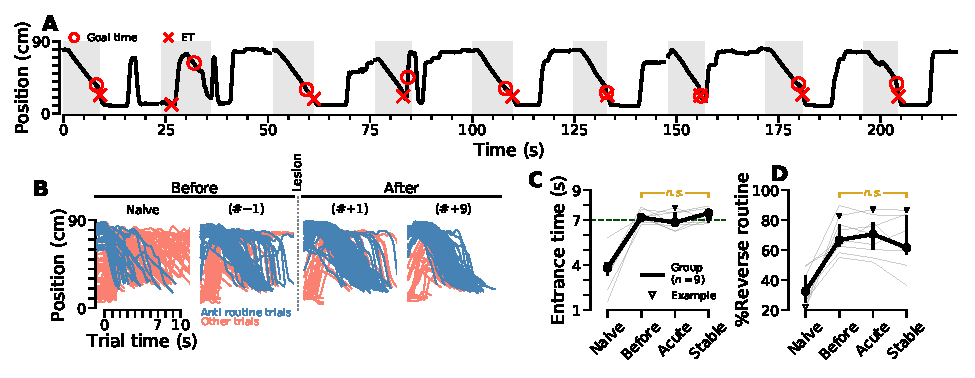
\includegraphics[width=\textwidth]{ch-lesion/figures/ReverseTreadmill.pdf}
	\caption[Preserved Motor Routine Performance After Lesion]
	{\textbf{Preserved performance of the run-and-wait routine following striatal lesion.}
	\textbf{(A)} Trajectory of a proficient animal trained in a version of the timing task in which the belt moved toward the reward area (rather than away from it). 9 consecutive trials and intertrials are shown.
	\textbf{(B)} Trajectories from a single representative animal in two sessions before and two sessions after lesion.
	\textbf{(C-D)} Comparison of ET (C) and percentage of run-and-wait routine usage (D), before and after striatal lesion.
	}
	\label{fig:lesion:rev}
 \end{center}
\end{figure}
If the striatal lesion abolished the ability to perform this motor routine, we expect animals to start the trials close to the reward area, at least in the first post-lesion sessions.
On the contrary, the performance of the run-and-wait routine was spared by striatal lesions (\Autoref{fig:lesion:rev}{C-D}).
It is noteworthy that lack of effect of the striatal lesion on the performance of the motor routine could be due to the fact that learning the reverse treadmill task was easier than the normal treadmill task, thus the relearning procedure might have happened during the very first session after the lesion.
This is unlikely to be the case since initial learning of the reverse treadmill task took a similar learning curve compared to that of the normal treadmill task (\autoref{fig:appendix:revLearn}).
Altogether, these results indicate that the striatum is not required to initiate or execute the sequential steps of the learned motor routine, but it is critical to invigorate its reward-oriented running phase.


\section{Intact Motor Function}
\label{ch:lesion:motorOk}

To better understand the origin of this vigor deficit, we examined whether striatal lesions affected elementary motor abilities of the animals.
First, we tested basic locomotor activity in a novel environment without any rewards.
We tracked their position during the first 10~min of exploration in a novel treadmill (without any food or water restriction prior to this test, see \autoref{ch:methods:loco} for more details).
Rats with \gls{dls} lesions had an identical amount of displacement on the treadmill compared to the control ones (\Autoref{fig:lesion:motorOk}{A}).
Thus, basic locomotion is spared by lesion of the striatum.
Then, we aimed to examine whether lesioned animals have the ability to outrun the treadmill, i.e., run faster than $\sim$10~cm/s.
We progressively increased the treadmill speed across 30~s long trials, interleaved by 30~s long intertrials.
Same groups of animals as in the last test ($n=12$ rats) performed similarly in this free running task (\Autoref{fig:lesion:motorOk}{B}).
Therefore, lesioned animals are able to run at speeds much faster than 10~cm/s if they are forced to.
Of note, the average speed of animals with a striatal lesion during the trials was similar to normal rats, but only for slower treadmill speeds.
\begin{figure}[bth!]
 \begin{center}
	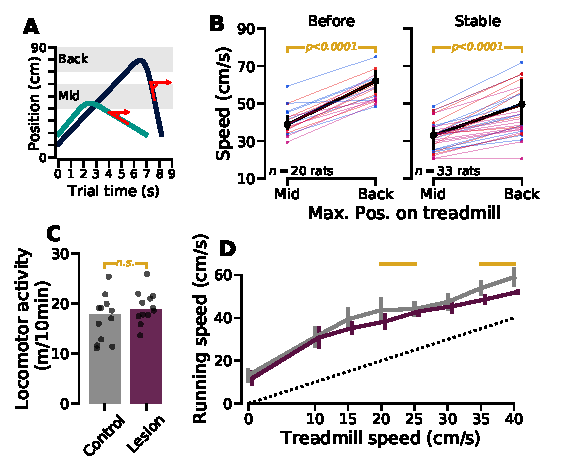
\includegraphics[scale=1]{ch-lesion/figures/MotorPreserved.pdf}
	\caption[Preserved Motor Control After Striatal Lesion]
	{\textbf{Preserved modulation of running speed and spontaneous locomotor activity following striatal lesion.}
	\textbf{(A)} Average speed when rats ran toward the reward area. Data were split according to the position of the rats on the treadmill when initiating their runs.
	\textbf{(B)} Speed of runs initiated either in the back or the middle portion of the treadmill calculated for each animal on the last 5 sessions before lesion (left) and sessions \#4 to \#9 after lesion (right).
	\textbf{(C)} Distance ran while exploring a new immobile treadmill for non-lesioned and lesioned rats ($n=12$).
	\textbf{(D)} Average running speed in a free running task (no reward) in which control and lesioned rats were submitted to trials with incremental treadmill speed (same color code as in C).
	Horizontal golden lines indicated significant differences between groups.
	}
	\label{fig:lesion:motorOk}
 \end{center}
\end{figure}
In trials in which the treadmill moved faster than 20~cm/s, even though lesioned rats managed to keep running, their speed had the tendency to be marginally slower than control animals.
This effect mimics the overall tendency of the animals to `choose' a slower pace, be it in approaching the reward area or starting to lick the available reward.
Next, we dived into the speed profile of the animals to investigate the essential ability of modulating the running speed.
We compared their running speed in trials in which the running epoch was initiated from the rear portion of the treadmill, versus the middle of the treadmill (in \Autoref{fig:lesion:motorOk}{C}: Back vs. Mid).
Non-lesioned animals ran faster when they initiated their runs from the back of the treadmill (\Autoref{fig:lesion:motorOk}{D}).
Interestingly, this modulation, too, was maintained after striatal lesions, although running speeds were generally slower following the lesion.


\section[Preserved Routine Learning]{(Mostly) Preserved Routine Learning}
\label{ch:lesion:learn}
Our results indicate that the \gls{ds} is not required for the execution of motor routines (at least those similar to the wait-and-run), rather it is influencing kinematics of learned behaviors.
Performing striatal lesion prior to learning the task, i.e., in na\"{i}ve animals, further confirmed earlier results.
We found that striatal lesions performed in na\"{i}ve rats did not compromise their ability to learn the wait-and-run routine (\Autoref{fig:lesion:EarlyLesionLearning}{A}).
Both groups of animals, with lesion in either \gls{dls} or \gls{dms}, learned the task with similar profile to control (non-lesioned) rats.
\begin{figure}[bth!]
	\begin{center}
		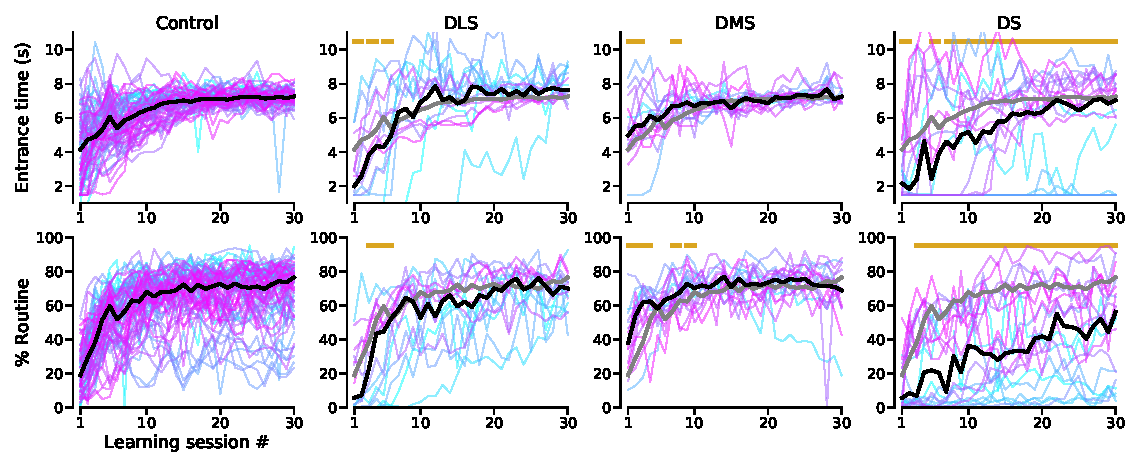
\includegraphics[width=\textwidth]{ch-lesion/figures/EarlyLesionLearning.pdf}
		\caption[Effects of Striatal Lesions on Learning]
		{\textbf{Effect of DLS, DMS and DS lesions performed before training on task learning.}
		\textbf{A)} Session-by-session change in performance ($ET$, upper panels; Percentage of trials in which the routine was used, lower panels) for animals without lesion (Control, \textit{left}) and for animals that received a lesion before training (DLS, DMS, DS from left to \textit{right}).
		Black lines indicate Control group median.
		Thin colored lines indicate single animals.
		Thick colored lines (same color code as in \autoref{fig:lesion:task}) in 3 rightmost columns indicate group performance for comparison (8 lesion animals with fewer than 30 training sessions are not shown, which explains the difference in the number of animals in this figure and \autoref{fig:method:LesionSizeLocation}).
		Horizontal golden lines indicate significant differences between control and lesion groups (corrected for multiple comparisons).
		\textbf{B)} Trajectories before and after extensive training (sessions \#1 and \#30) for two animals with large DS lesions.
		Note that, after extensive practice, R238 was capable of performing the wait-and-run routine.
		\textbf{C)} Percentage of trials in which animals remained in the front region of the treadmill (computed for sessions \#25 to \#30) versus lesion size.
		}
		\label{fig:lesion:EarlyLesionLearning}
	\end{center}
\end{figure}
Those animals with lesion in the entire \gls{ds}, however, showed a different trait.
A few of them with relatively larger lesion, failed to display performance improvement (\Autoref{fig:lesion:EarlyLesionLearning}{A}).
All of these animals ran most of the time in the front region of the treadmill (\Autoref{fig:lesion:EarlyLesionLearning}{B,~C}).
The rest of this group, similar to the \gls{dls} and \gls{dms} groups, eventually improved their performance.
In animals with striatal lesion performed before training, a robust reduction of running speed was also observed, an effect that was correlated with lesion size as well (\Autoref{fig:appendix:spd}{B}).


\section{Effort, The Underlying Mechanism}
\label{ch:lesion:effort}
\begin{figure}[bth!]
	\begin{center}
		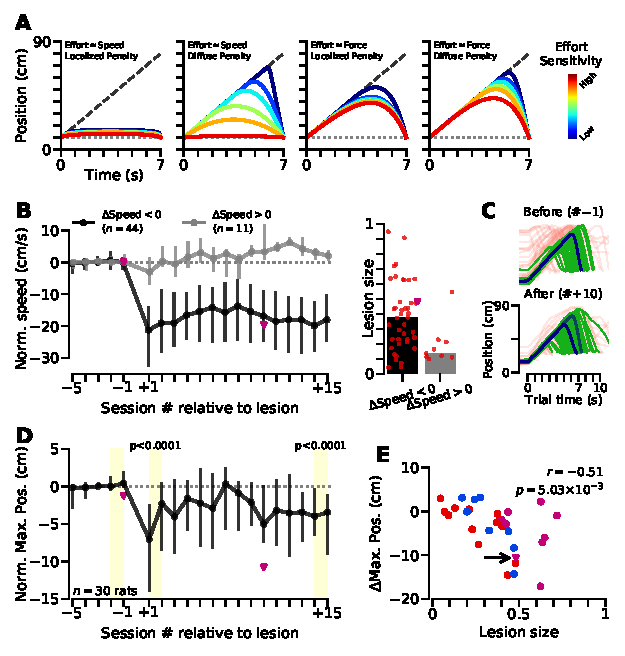
\includegraphics[scale=1]{ch-lesion/figures/MaxPosAnalysis.pdf}
		\caption[Optimal Trajectory and Experimental Validation]
		{\textbf{Optimal trajectory vs.\ effort sensitivity and experimental validation.}
		\textbf{A)}
		Optimal trajectories predicted by models with different effort and spatial costs approximations.
		The cost of premature entrance in the reward area (spatial cost) was simulated using a Heaviside function that was either localized ($\sim$step function with non-zero value within the reward area) or diffuse ($\sim$a sigmoid function whose value gradually decreases toward zero away from the reward area).
		Effort was approximated as the square value of either the modeled muscular force produced by the animals or of its speed.
		\textbf{B)}
		\textit{Left}: animals were divided into two groups based on the impact of the striatal lesion on their running speed.
		\textit{Right}: lesion size for animals in those two groups.
		Green triangles in panels~B,~D, and~E are data points from the example animal whose trajectories, before and after lesion, are shown in panel~C.
		\textbf{C)}
		Effect of striatal lesion on the trajectories of a single animal.
		Only trials in which the routine was executed (thin blue lines) were taken into account to find the trajectory of median maximum position (tick blue line).
		The shadow of the trajectory of median maximum position before lesion is displayed in the bottom plot for comparison.
		\textbf{D)}
		Effect of striatal lesion on the median maximum position in routine trials.
		\textbf{E)}
		Effect of striatal lesion on the median maximum position vs.\ lesion size.
		Same color code for individual lesion type as in \autoref{fig:lesion:task}.
		}
		\label{fig:lesion:maxPos}
	\end{center}
\end{figure}
Since the striatal lesion spared the rats' ability to learn the motor routine, execute it, and modulate their running speed, the most parsimonious account of our results is that lesioned animals `preferred' slower speeds.
We took advantage of the optimal control framework that relies on the assumption that animal behavior is optimal with respect to a cost function.
A simple model was implemented to simulate the optimal trajectory taking into account costs related to energy expenditure (effort) and those imposed by the task rules (running in the front is costly as it leads to premature \gls{et}, which is punished).
Four cost functions were used to model speed/force-based effort, and localized/diffuse penalty related to staying in the front of the treadmill (see \cite{JuradoParras2020} for more details).
We found that higher effort sensitivity, regardless of exact cost function parameters, resulted in optimal trajectories with smaller `maximum position', i.e., earlier run-phase initiation (\Autoref{fig:lesion:maxPos}{A}).
Hence, combination of late initiation of the run-phase together with fast running speeds was not used.
This result is not only in agreement with the reduced running speed observed following the lesion, but is also reminiscent of the behavior observed during the very first post-lesion sessions, when animals with larger \gls{ds} lesions ran mainly close to the reward area (\Autoref{fig:lesion:task}{F,~G}). 
We thus reanalyzed the effect of striatal lesion on the trajectory, focusing on animals with a significant reduction in running speed (\Autoref{fig:lesion:maxPos}{B}).
We also limited the analysis to trials during which animals perfectly executed the wait-and-run routine, since those are the trials for which defining the maximum position is relevant.
Strikingly, following striatal lesions of various sizes and locations, rats started running forward earlier relative the length of the treadmill, i.e., a smaller maximum position (\Autoref{fig:lesion:maxPos}{D}).
This effect too, similar to speed, persisted after three weeks of daily sessions post-lesion.
Also, the reduction in maximum position was well-correlated with lesion size, the bigger the lesion, the bigger the reduction (\Autoref{fig:lesion:maxPos}{E}).
\glsresetall
\chapter{Discussion}
\label{ch:discussion}
In this chapter, for each set of experiments, I will first summarize the results, and then discuss their more general implications.
Then I present a short conclusion of the entire work, trying to reconcile all the ideas.
Next, I will describe some of the weak points from which I think this work might be suffering.
Finally, some ideas and directions for my future-self are presented that can complement and strengthen this manuscript.


\section{Time Estimation}
\label{ch:disscusion:time}

In this study, we used a treadmill-based behavioral assay in which rats, once the treadmill started moving, were required to wait for 7~s before approaching the reward location.
Objectively, animals may accurately time their approaches using either one of the following two mechanisms:
\begin{enumerate}[noitemsep, label=\Roman*.]
    \item They may rely on a purely \textit{internal} mechanism (e.g., self-sustained neuronal dynamics read by their motor system) to learn how long they should wait and decide when to approach the reward port.
    In this case, performance accuracy should be largely independent of variations in \textit{external} factors (e.g., the speed of the treadmill, the animal position on the treadmill at trial onset,\ldots).
    Additionally, to save up energy, animals would probably stay close to the reward area for most of the duration of the trial.
    \item Animals may discover, by trial-and-error, a motor routine adapted to the apparatus and task parameters, whose complete execution would take them into the reward area at the right time, i.e., around the \gls{gt}.
    In this case, timing accuracy would be related to the stereotyped performance of that routine and should heavily depend on task-specific features of the environment or the order of the elements composing the motor sequence.
\end{enumerate}
The dominance of either of the algorithms can be directly inferred from behavioral experiments in which critical task parameters are manipulated.
The results of our behavioral experiments clearly favor the latter embodied strategy.
Using two distinct reinforcement learning-based agents that either incorporated or lacked time representation, we showed that the behavior of our animals is incompatible with them accessing an internal explicit knowledge of elapsed time~\cite{Safaie2020PNAS}.
\par
We report that to accurately wait 7~seconds before approaching the reward port, most rats developed the following ``wait-and-run'' motor routine.
First, they waited for the beginning of each trial in the reward area.
Then, upon trial onset, they stayed relatively still while the treadmill carried them to the rear wall of the treadmill.
Finally, as soon as they reached the back of the treadmill, they ran straight to the reward port, without pause.
In this experimental `control' condition (see \autoref{ch:time:treadmill}), the accuracy of the animals reached its peak after 15~to 20~training sessions.
However, even for proficient animals, the probability of performing a correct trial was almost null when they started a trial in the back region of the treadmill.
In addition, when animals started a trial in the reward area, performing a correct trial was almost exclusively associated with the animals reaching the back portion of the treadmill.
Finally, following extensive training in the control condition, when we modified the task parameters to penalize the stereotyped performance of this front-back-front trajectory, the behavioral proficiency and accuracy of the animals dropped dramatically.
These results support the hypothesis that, in our task, performing the motor routine is necessary for accurate performance.
\par
It could be argued that the animals' tendency to develop this front-back-front trajectory resulted from the structure of the task that provided an easy solution that animals used instead of estimating time while continuously running just behind the infrared beam.
In other words, had the task not favored the usage of an readily available motor routine, rats might have timed their reward approaches by relying on an internal representation of time that might have arisen from the ability of recurrent neural networks to generate self-sustained time-varying patterns of neural activity~\cite{Buonomano2011chapter}.
With several additional experiments we showed that rats have limited ability to use an internal representation of time when the task parameters are set such as to prevent the usage of a stereotyped motor sequence to solve the task.
\par
First, we trained a group of animals while the treadmill speed randomly changed every trial (see \autoref{ch:time:varSpeed}).
Compared to animals trained in the control condition, those trained with variable speed were less accurate.
Additionally, these animals attempted to use the same front-back-front trajectory, evident by an increased probability of correct trials when the treadmill speed allowed it.
Second, we trained a different group of rats in a version of the task that penalized them when they started the trials in the reward area (see \autoref{ch:time:nto}).
In this condition, solving the task is not possible using the usual routine and rats trained in this condition displayed strong accuracy impairment.
Moreover, they kept trying to develop a modified front-back-front trajectory and started the trials as close as possible to the infrared beam (note that the infrared beam location was not marked).
In all the above experiments, during trials, the treadmill pushed the animals away from the reward area which favors the usage of the wait-and-run routine.
To avoid this possible bias, in our last experiment, we trained a group of rats on an immobile treadmill (see \autoref{ch:time:immobile}).
Rats' performance was poor in this condition, with some animals failing to show any signs of learning, and others failing to reduce their variability.
The increased variability is likely to result from the fact that, when the treadmill is immobile, a motor sequence to fit in 7~s is more difficult to be reproduced reliably across trials, rather than in the control condition in which most of the sequence is a passive wait on the treadmill until the animal reached the rear wall.
Moreover, we noticed that the best rats in the immobile treadmill condition systematically ran to the back region of the treadmill where they performed a series of rearing and wall-touching movements, just before crossing the treadmill toward the reward area.
With our video tracking system, we could not quantify these movements, however, by visual inspection, I speculate that those movement were also rather stereotypical, not unlike those reported by~\citeauthor{Kawai2015} in~\cite{Kawai2015}.
Altogether, we conclude from this set of experiments that rats, forced to wait for several seconds before approaching the reward, did not seem capable of using a purely internal and disembodied representation of time, but always attempted to develop a motor routine in the confined space of the treadmill, a routine whose execution duration amounted to the time they needed to wait.
This conclusion was also supported by the experiment whereby animals were less accurate in timing their entrance in the reward area when the \gls{gt} was set to 3.5~s, compared to the control \gls{gt} of 7~s.
Indeed, in this short~GT condition, the wait-and-run strategy is not optimal, as animals would enter the reward area too late.
Thus, the increased variability might be explained by the difficulty for the rats to ``self-estimate'' when to start running forward without the help of a salient sensory cue (such as touching the back wall).
In support of this idea, in 67\% of the error trials, the rats started running forward before reaching even the middle of the treadmill.
In addition, a few animals trained in the short goal time condition developed a new stereotyped motor sequence, i.e., running from front to back and back to front.
Interestingly, their \glspl{et} were less variable than animals that remained immobile after trial onset and tried to estimate when to run forward in the middle portion of the treadmill.
\par
A practical limitation of our work is whether its conclusion is relevant beyond the specifics of our experimental protocol, i.e., a suprasecond long motor timing task in which the rewarding action is a locomotor activity, not a distinct response (e.g., a lever press).
Interestingly, in a study in which a group of rats had to perform two lever presses interleaved by 700~ms, each animal developed an idiosyncratic motor sequence\footnotemark\ lasting precisely 700~ms~\cite{Kawai2015}.
\footnotetext{
    Consider the following as an example:
    1\#~press the lever with the left paw;
    2\#~touch the wall above the lever twice with the right paw;
    3\#~second press on the lever with the left paw.
}
The large inter-individual variability reported in this study may arise from the multiple possibilities of simple action sequences that can be squeezed in such a short time interval and easily reproduced across trials, taking advantage of the proximity of the front wall and lever.
If the time interval was longer, all the animals might have developed the same motor sequence (e.g., running back and forth in the experimental cage between the two lever presses).
Nevertheless, this study provides an additional example in which virtually all animals developed a motor strategy, even if compared to our task, the time interval was much shorter ($<$1~s) and the terminal operant response was distinct (a single lever press).
It is well-known that temporal regularities in animal conditioning protocols favor the development of automatic motor sequences.
In one of the rare studies that continuously recorded and quantified the full body dynamics of rats performing a sensory duration categorization choice task, authors reported that animals developed highly stereotyped motor sequences during presentation of the sensory cues and that perceptual report of the animals could be predicted from these motor sequences~\cite{Gouvea2014}.
Thus, animals use embodied strategies in tasks requiring them to categorize (short or long) the duration of time intervals too, suggesting that our results are not just due to the particularities of the task.
Moreover, these results are in line with an earlier study showing that the prediction of rats' temporal judgment (a 6~s long versus a 12~s long luminous signal) was always better if based on the collateral behaviors performed by the animal at the end of the signal than if based on the actual time~\cite{Fetterman1998BehProc}.
In such temporal discrimination tasks, a stereotyped sequences of movements (collateral behavior) might serve as an external clock and the choice of the animals might be primarily determined by what the animal is doing when a sensory cue disappears rather than by an internal estimation of the duration of that cue.
That timing could be primarily embodied might seem counter-intuitive with our innerly-rooted feeling of time.
Nonetheless, humans display poor temporal judgment accuracy when prevented to count covertly or overtly~\cite{Rattat2012} and several studies have reported that movements improve the perception of intervals~\cite{Su2012,Manning2013,Wiener2019eNeuro}
It has been recently proposed that the explicit perception of time in humans may be constructed implicitly through the association between the duration of an interval and its sensorimotor content~\cite{Coull2018}.
Embodied timing, by replacing time per~se with various processes depending on tasks and contexts, explains why such a diverse set of brain regions, including but not limited to the prefrontal cortex, motor cortex, \gls{bg}, cerebellum, \gls{sma}, entorhinal cortex, and hippocampus have been associated with time representation~\cite{Pouthas2005, Kraus2013Neuron, Bakhurin2017JNeuro, Morillon2017PNAS, Gu2018NeuroLearnMem, Mello2015, Schubotz2000, Heys2018NN,JazayeriNN2018}.\footnote{In my opinion, the fact that this many brain structures have been implicated in timing should, in and of itself, raise more questions than it answers.}
% The novelty of our work is, first, to demonstrate that even in conditions that discourage the use of such motor strategies rats do not seem able to rely on a purely internal timing mechanism and, second, that a critical determinant of temporal accuracy is the possibility to develop motor routines that can be guided by interactions with salient features of the environment.
\par
It has been previously proposed that timing could be mediated through motor routines whose precise execution is internally controlled~\cite{Killeen1988,Dragoi2003, Staddon1999}.
So, one could argue that accurate timing in our task was also ultimately driven by internal neuronal dynamics.
I must stress that our conclusion that animals rely on an embodied strategy, rather than internal neuronal clocks (dedicated or emergent), does not mean that internal brain activity is irrelevant to well-timed behavior.
We do not question that representations/correlations of elapsed time have been observed in individual and population neuronal activity in various brain regions during time-constrained tasks or that perturbation of neuronal activity impairs timing accuracy.
For example, in a novel task where head-fixed mice learned to remain still for 6~s before accelerating toward the reward at the end of a virtual track, multiple \textit{time cells} were identified in the entorhinal cortex that were sequentially active during the interval, and scaled proportional to the waiting time~\cite{Heys2018NN}.
Mice during the immobility period did not have any locomotor activity (they had subthreshold locomotion), and there is no other behavioral report.
I would confidently say, based on my limited experience with rodents, that no mouse remains frozen for 6~s.
Temporal correlations, in turn, could be covariates of any other motor activity.
Similarly, \Citeauthor{JazayeriNN2018} found temporally scaling dynamics during a timing task in both the prefrontal cortex \textit{and} the \gls{dms} of monkeys~\cite{JazayeriNN2018}.
This type of results can not be used as definitive evidence in favor of a neuronal clock, \emph{read} by animals as we, humans, read a clock~\cite{Krakauer2017Neuron, Buzsaki2017SciRev, Buzsaki2018TICS}.
Our behavioral results are not easily compatible with the idea that neural representations of time are a signature of a \emph{clock-like} algorithm for time estimation.
Rather, they are compatible with the idea that timing emerges from the dynamics of neural circuits~\cite{Paton2018NeuronRev}, as long as these dynamics are not assumed to be entirely internally generated and also reflect feedback from the environment.
For instance, I speculate that the timing deficits induced by striatal inactivation in a similar version of the treadmill task~\cite{Rueda2015NN} might be explained by considering the role of this brain region in accumulating sensory information before taking a decision, or in invigorating the ongoing behavior~\cite{Yartsev2018eLife,Dunovan2016FrontNeurosci}---more on the role of the striatum later on.
In our experimental setting, one could assume that rats, by gathering sensory evidence, decide when to start running and how fast.
Thus, it may be relevant to consider the process governing when the rats will run forward as an accumulation of sensorimotor evidence.
The \gls{ds} is critical for processing sensorimotor information~\cite{Robbe2018} and has been proposed to contribute to the process of evidence accumulation during decision making~\cite{Yartsev2018eLife}.
Interestingly, it has been recently proposed that a competition between the direct and indirect \gls{bg} pathways, tuned by \gls{da} modulation, may determine the speed of evidence accumulation toward decision taking~\cite{Dunovan2016FrontNeurosci}.
Such a model predicts an increase (\textit{decrease}) in \gls{da} activity will speed up (\textit{slow down}) the accumulation of sensorimotor information and will lead to an early (\textit{delayed}) response.
% A recent study validates this model in mice performing an auditory duration categorization task, showing that increased \gls{da}ergic activity in the \gls{snc} was associated with the animals perceiving long tones as short ones~\cite{Paton2016Sci}.
\par
In conclusion, I point out that the embodied mechanism for motor timing is the most parsimonious, can explain a large body of experimental data, and by taking advantage of modern tracking technologies~\cite{DeepLabCut2018NN}, can potentially be applied in other types of time-estimation tasks.
By adopting the embodiment perspective, I raise the question that while animals naturally use motor strategies in time-constrained situations, why should there exist an independent internal clock?
\section{Striatal Function}
\label{ch:disscusion:lesion}

The striatum can powerfully influence the production of purposive movements.
Indeed, it is well-known that striatal dysfunction is the primary cause of the motor impairments (akinesia, bradykinesia, levodopa-induced dyskinesia) seen in \gls{pd}~\cite{Mink1996,McGregor2019Neuron}.
In addition, activation of striatal \glspl{msn} forming the direct (indirect) \gls{bg} pathway facilitates (prevents) movement production through disinhibition (inhibition) of brainstem and forebrain motor regions~\cite{Kravitz2010Nature}.
This fundamental feature of the \gls{bg}'s functional anatomy combined with recordings and perturbations of striatal activity in various behavioral tasks, has led to three prevailing hypotheses regarding how the striatum contributes to the control of purposive movements: %#TODO: define purposive movement in a footnote
\begin{itemize}[noitemsep]
    \item the selection/repression of actions~\cite{Barnes2005Nature, Cui2013Nature, Klaus2017Neuron, Markowitz2018Cell};
    \item the moment-to-moment generation of overlearned motor sequences~\cite{Dhawale2019};
    \item and the modulation of movement speed~\cite{Kim2014EJN, Rueda2015NN, Barbera2016Neuron, Yttri2016Nature, Panigrahi2015}.
\end{itemize}
The validity of these hypotheses is debated~\cite[for instance, see][]{Dudman2016CurrOpinNeurobiol} and, interestingly, they face common shortcomings.
For example, they fall short of explaining why lesioning or inactivating striatum's anatomical targets (i.e., the \gls{bg} output nuclei) in non-human primates only marginally alters the execution and speed-profile of overlearned motor sequences~\cite{Desmurget2010JNeurosci}; it even alleviates motor deficits observed in \gls{pd} patients~\cite{Turner2010CurrOpinNeurobiol}.
Moreover, in behavioral tasks typically used to probe the striatal motor function through perturbation of neuronal activity, it is next to impossible to disentangle whether failure to perform is due to inability to implement a decision into movement, or due to an impairment in higher-level processes (e.g., sensory processing and decision making), despite functional motor systems.\footnotemark
\footnotetext{
    This is referred to as the \emph{performance confound}.
    I only understood this concept after my supervisor came up with this rather bitter example:
    \textit{Imagine you cut up someone's legs and then say that they \underline{cannot} learn to run.}
}
\par
In this part of the study, we aimed to understand how the striatum contributes to the control of purposive actions, while limiting the performance confound as much as possible, we took advantage of the behavior displayed by animals in the treadmill task.
This task was identical to the one used in the time experiments under the `normal' condition (\Autoref{fig:methods:taskRules}{a}, and \Autoref{fig:lesion:task}{a}).
We trained a group of animals, including the same animals presented in \autoref{fig:time:CtrlTrd}.
They mostly developed the wait-and-run routine on the treadmill (but also see \autoref{fig:appendix:BadCtrl}).
After their performance on the task plateaued, they were randomly assigned to striatal lesion groups in different areas:
    \gls{dls}, \gls{dms}, or the entire \gls{ds}.
Excitotoxic lesions, the kind we used here, compared to lesions induced by electrical currents, have the benefit of sparing the passing fibers.
Moreover, due to their permanent nature, they are probably a more direct way to assess the function of the manipulated area~\cite{Otchy2015Nature}.
Following the lesion, animals were allowed to recover for $\sim$2~weeks.
After this recovery period, visually, they had normal behavior in their homecage.
Then, they resumed the training with identical task parameters to the sessions prior to the lesion.
After the striatal lesion, most animals could still perform in the task, with comparable proficiency to that of the pre-lesion sessions.
In addition, motivation does not seem to be affected, since the animals still engaged in the task, and consumed the reward in correct (and thus rewarded) trials (\autoref{fig:lesion:lick}).
The most striking effect was a marked reduction in the running speed toward the reward.
This slowdown was irreversible (\Autoref{fig:lesion:task}{J}) and well-correlated with the size of the lesion (\Autoref{fig:appendix:spd}{A}).
Interestingly, animals with reduced speed, also started to run earlier toward the reward, i.e., the maximum position of their trajectories was smaller.
This trait was also well-correlated with the lesion size and was also irreversible (\autoref{fig:lesion:maxPos}), but not trivial to explain using the aforementioned models of the striatal function (more on this later).
\par
Noticeably, in a number of animals, arguably the ones with relatively larger lesions, executing the routine was impaired for the first few sessions ($\sim<$5), and recovered afterward.
They mostly stayed in front of the infrared beam and committed many error trials.
It could be argued that the lesion prevented the performance of the motor routine, and especially animals with larger lesions stayed in the front since it is associated with the reward, evident by the strong preference for the reward area in both na\"{i}ve and trained rats (\autoref{fig:appendix:initPos}).
This is also in line with the second hypothesis cited above by \citeauthor{Dhawale2019}~\cite{Dhawale2019}.
To further investigate this possibility, we designed a variant of the task to directly evaluate whether lesioned animals lose the ability to perform a motor routine (or at least a comparable motor routine).
In this `reverse' treadmill task, the conveyor belt moved toward the reward area.
Animals could just move to the back of the treadmill during the intertrial (while the treadmill motor was turned off, this would be a simple locomotion which was not affected in lesioned animals) and upon trial start, stay still while the treadmill carried them to the reward area at the right time (\gls{et}~$=$~\gls{gt}).
Importantly, impaired execution of this ``run-and-wait'' motor routine could be clearly observed, because the animals should similarly stay in the front.
However, experimental data showed otherwise, animals kept performing the routine with no sign of deficiency.
These results demonstrate the spared ability of animals to perform motor routines.
\par
We also formally confirmed normal locomotor activity by measuring the total displacement during the first 10~min in an unfamiliar environment (\Autoref{fig:lesion:motorOk}{A}).
Furthermore, we investigated whether lesioned animals are able to run at faster speeds.
Some of the control and lesioned animals were tested in a new paradigm, consisting in trials of 30~s followed by intertrials of 30~s.
There was no reward available and the speed of the treadmill progressively increased across trials (see \autoref{ch:methods:loco} for details).
Interestingly, lesioned animals were capable of running at speeds much higher than the treadmill speed---up to 40~cm/s compared to the treadmill speed of 10~cm/s (\Autoref{fig:lesion:motorOk}{B}).
Similar results have been reported in \gls{pd} patients using different behavioral tasks~\cite{Mazzoni2007, Schmidt2008Brain}.
Another possible explanation of our data may be lack of more general motor control abilities, such as modulation of speed.
For example, it has been previously shown that the speed of reward-oriented movements increases with movement distance to minimize the \gls{cot}~\cite{Shadmehr2010Jneurosci}.
In our task, one could argue that an animal with a limited range of locomotion speed at its disposal, would prefer a shorter running epoch with a constant slow pace, to a longer one with more complex speed dynamics (\Autoref{fig:lesion:motorOk}{C}).
By further analysis of our data, we observed that, for every single control animal, trials with higher maximum position were indeed faster (\Autoref{fig:lesion:motorOk}{D}).
Importantly, this effect was preserved after striatal lesion, although all the speeds are generally lower than control animals.
These results show that animals' elementary ability to modulate their locomotion speed was maintained.
\par
Overall, our results indicate that rats with striatal lesions did not display fundamental impairment in motor control or action selection.
After striatal lesion, animals kept arriving on time in the reward area, but they started to run earlier (i.e., from a more frontal portion of the treadmill) and they ran at a slower velocity.
Running at slower speeds could be explained by current models of striatal function, but the tendency to start running early is surprising.
Alternatively, animals could have reached similar positions on the treadmill and still used a slower speed to approach the reward.
The major disadvantage of this hypothetical strategy may be a longer running distance which incurs more energetic cost.
Indeed, optimal control models predicted that higher sensitivity to energy expenditure (effort) leads to a similar strategy: starting to run earlier and slower~\cite{JuradoParras2020}.
Our results thus support the view that the striatal lesion increased the animals' sensitivity to effort which led them to modify the kinematics of the wait-and-run routine.
In other words, our work suggests that \gls{ds} contributes to the generation of an effort signal that influences the kinematic parameters of purposive actions.
Metaphorically speaking, the same effect would have been expected had we forced control rats to perform the task with extra weight on their back.
Such a function is congruent with the hypothesis, derived from \gls{pd} patients, that \gls{da} projections to the striatum provide a signal for implicit motor motivation (or global effort sensitivity), which influences the vigor of goal-directed movements~\cite{Mazzoni2007}, and lack thereof causes bradykinesia.
How exactly the progressive degeneration of \gls{da}ergic neurons in \gls{pd} results in bradykinesia is difficult to establish, in spite of evidence in a mice model of \gls{pd} supporting a critical role of \gls{da} in the \gls{ds} for the control of movement vigor~\cite{Panigrahi2015Cell}.
On the other hand, whether the \gls{ds} is critical for action selection/initiation/repression has been an important topic of debate~\cite{Turner2010CurrOpinNeurobiol, Dudman2016CurrOpinNeurobiol}. 
In this context, our study provides compelling evidence for a specific role of the \gls{ds} in setting the sensitivity to effort expenditure.
Our results indicate that striatal lesions changed the kinematics of a well-learned motor routine as a result of increased sensitivity to effort, without altering the animals' capacity to run at different speeds.
Selective perturbation of the activity of striatal projection neurons bidirectionally modulates the speed of goal-directed movements~\cite{Yttri2016} and spontaneous locomotion~\cite{Kravitz2010}. 
Our results complement these studies by suggesting that the \gls{ds} is not the primary controller of movements, but provides a second layer of modulation that tunes their kinematics according to cost/benefit considerations.
More generally, the role of the \gls{ds} in contributing to the cost/benefit analysis of actions has repercussions beyond the modulation of ongoing movements as it can also explain why manipulations of striatal activity change the preference for certain actions~\cite{Kravitz2012NN}, bias decision making~\cite{Tai2012NN} or alter the retrieval of procedural memories \cite{Geddes2018Cell}.
Expending effort to produce faster movements allows limiting the \gls{cot} as well~\cite{Shadmehr2019TINS}.
In sensory guided decision-making tasks, the \gls{cot} can also be reduced by limiting the duration of deliberation~\cite{Carland2019NeuroSci}.
Interestingly, recent evidence supports a specific role of the \gls{bg} in signaling the urgency to commit to an action choice~\cite{Thura2017Neruon,Carland2019NeuroSci}.
Thus, our proposed function of the \gls{ds} might provide a common framework to reconcile seemingly conflicting findings across motor control and decision-making fields.
\section{Conclusion} \label{ch:discussion:conclusion}

In short, accurate timing requires stereotyped interaction with the environment and the striatum determines the effort invested in this interaction~\cite{Safaie2020PNAS,JuradoParras2020}.
\par
That the perception of elapsed time is somehow related to the movement of things is not a surprise to anyone.
In this work, however, we attempted to determine the necessity of movements.
In other words, whether there is an internal mechanism which can provide a measure of time that drives behavior, or time is perceived through actions that fill the interval of interest.
Multiple experiments designed to interfere with the usage of stereotyped motor routines, all led to drastic decline in temporal accuracy.
These results suggest that the hypothetical internal timer does not suffice to produce a timely motor response in the suprasecond timescale.
We thus argue that time intervals in the brain may be represented with the movements that happen to take that long to execute.
% In turn, temporal control of individual sub-actions in a complex movement presents a different timing problem, which is not only in a much shorter timescale (tens of milliseconds, instead of seconds), but also it's constrained with the mechanical characteristics of the body (e.g., mass, leg length,\dots).
Thus, the problem of time perception is translated to a motor control problem, learning and performing adaptive motor routines.
\par
The \glsentrylong{ds} has been implicated in initiation and selection of movements, as well as in controlling their speed.
We took advantage of the wait-and-run motor routine, consistently developed by animals in the treadmill task, to delineate the role of the striatum.
Using a number of original tasks, for a large group of animals, we illustrated that permanently lesioning different areas of the dorsal striatum does not affect neither the ability to learn the motor routine by trial and error, to perform the learned motor routine, to run fast, to modulate the running speed as needed, nor the motivation to acquire the reward.
However, lesioned animals robustly performed a less effortful routine by waiting less and running slower, two traits that well-correlated with the size of the lesion.
Hence, we propose that the main motor function of the striatum may be setting the sensitivity to effort in purposive actions.
Such an elementary function has the potential to reconcile a large body of seemingly contrasting hypotheses. % Conclusion
\section{On the Other Hand}
\epigraph{The idea that the future is unpredictable is undermined every day by the ease with which the past is explained.}
{\textit{Daneil Kahneman, Thinking, Fast and Slow}}
\noindent
It is time to discuss some of the downsides of my thesis project, some possible flaws that might result in interpretive limitations.
First issue relates to the structure of the task.
The treadmill task does not require a clear and distinct operant response, rather the animal crosses the infrared beam, the location of which is unmarked and unknown to the animal.
This is uncharacteristic for a time-estimation task.
In retrospect, had we installed a simple lever or nose-poke above the reward port to register the entrance times, it would have provided a more straightforward timing task.
The task was originally designed to be used at faster speeds (30~cm/s) and such a mechanism was perhaps deemed impractical.
%======
Next point is also with regards to the task.
In its nature, I think, the treadmill task favors a motor strategy, and this might have biased our results.
Aside from the immobile condition, the treadmill always moves and so imposes a dynamic environment to the agent, an environment in which avoiding motor activity is not even possible, since eventually the animal would arrive to the back wall and \textit{has to} move.
The immobile condition was an attempt to remedy this problem.
Indeed, we showed that better performance was correlated with more movement along the treadmill and visually, I observed that our best-performing animal developed an stereotyped ritual in interaction with the back wall of the treadmill.
However, even in this condition, animals couldn't simply stay in the reward area, and presumably \textit{estimate} the goal time duration, at least they had to move a few centimeters backward to prevent premature interruption of the beam.
Ideally, to test the embodied view, the time-estimation task should not allow any motor activity, perhaps by penalizing movements however, a new problem arises:
what would be the ecological relevance of such a task, especially in suprasecond timescale?
And this is closely linked to my last remark.
Even though learning about embodiment and its implications immensely influenced my thinking, I fear that in the context of timing, it might be unfalsifiable.
For instance, even if human subjects are asked to not move at all during a time-estimation task, and they perfectly follow the protocol, one could argue (and I do argue) that they still mentally picture a motor activity or a moving object.
Overall, I think the best argument in favor of embodied time-estimation is its parsimony, and that adopting this perspective affords a great explanatory power.
\par
The lesion experiments are also not flawless.
One issue is that the quantity of reward progressively decreased for correct trials with later entrance times (\autoref{fig:methods:taskRules}).
Thus, had lesioned animals started running at a position similar to normal rats using a slower speed, they would have received a slightly smaller drop of reward.
The most skeptical reader might suggest that this is the reason why animals tend to wait less, to avoid smaller rewards.
However, the reward magnitude drops at a low rate, therefore I do not think a $\sim$5\% smaller reward is noticeable.
In any case, at least for the lesion experiments, a constant reward size after the goal time would have been preferred.
%======
Lastly, one issue that might have downgraded our effect sizes, especially with regards to the maximum position analysis, was the behavioral variability.
Some animals developed different strategies to solve the task (\autoref{fig:appendix:BadCtrl}).
At the time, to respect the natural repertoire of behavior, we indiscriminately carried on with the lesion experiments for all the animals.
Later on, while processing the data, I realized most outlier data points belonged to animals with strange pre-lesion behavior, but at this stage we did not have any excuse to exclude those animals, and we did not.
Instead, we explicitly set criteria for including animals in the maximum position analysis (\autoref{fig:lesion:maxPos}).
These criteria might seem arbitrary to some, although they served the purpose of the analysis and were set blind to the performance of individual animals.
I suppose performing the lesion only in animals that behaviorally conformed to the wait-and-run routine would have rid us of much of the \textit{extra} variability and would have been also justified.


\section{Future Work}
Thus far, I provided, hopefully, convincing evidence in support of the necessity of motor routines for accurate timing and that the \gls{ds} set the sensitivity to the expended effort in motor routines.
Then I discussed the limitations in the design of the task and the interpretation of our data, and now I propose some directions for future research.
\par
% We showed that lack of a simple motor strategy leads to the deterioration of timing performance.
% Therefore, if one considers a continuum for timing strategies on an embodied--internal axis, then, why the internal mechanism is less accurate than the embodied one?
% In the context of this work, I think the related question is: why 
We showed that the timing performance deteriorates in the absence of an \textit{easy} motor strategy, i.e., a motor routine that is adapted to the environment, like the wait-and-run routine in the control treadmill task.
The worst performances were observed in the versions of the task wherein stereotyped execution of a 7~s long motor routine was arguably the hardest, like the immobile condition, compared to the variable speed condition.
I would suggest that this is due to the inherent difficulty of reliably executing a suprasecond motor routine in a static environment, while in the control condition, the environment provides a reliable and salient cue, i.e., touching the back wall.
It remains speculative whether in the immobile condition (or any other conditions) animals developed a different idiosyncratic routine, either postural or with their limbs, that we couldn't capture with our position-tracking system.
Better behavioral quantification, possible with the advent of modern technologies such as \textit{DeepLabCut}~\cite{DeepLabCut2018NN}, in ecologically-valid timing tasks~\cite{VanRijn2018TICS} could detect such previously-unnoticed routines.
Furthermore, it also requires future investigations into theoretical reasons why inferring time from internal dynamics of neural networks seemingly results in higher variability than relying on physical interaction with the environment.
\par
In the second part, we used permanent fiber-sparing lesions to study the role of the striatum in development, execution, and control of the wait-and-run motor routine.
Lesion is a useful tool to establish a causal `instructive' function for the striatum~\cite{Otchy2015Nature}, however, it does not provide any information as to how direct-indirect pathways are involved.
Recent genetic tools allow pathway-specific perturbation of neural activity in rats~\cite{Pettibone2019eNeuro}, which is absolutely compatible with our task and setup and would complement our conclusions greatly.
I would speculate that direct (indirect) pathway stimulation would cause cost underestimation (overestimation), somewhat contrary (similar) to what we observed by lesions.





opto
DA manipulation

Future studies should investigate whether signaling effort and urgency are the two sides of a unique function implemented in the \gls{bg} to maximize the reward rate while minimizing costs. % Future work
\glsresetall
\appendix % all chapters following will be labeled as appendices
\chapter{Supplementary Figures}

\begin{figure}[!h]
  \begin{center}
    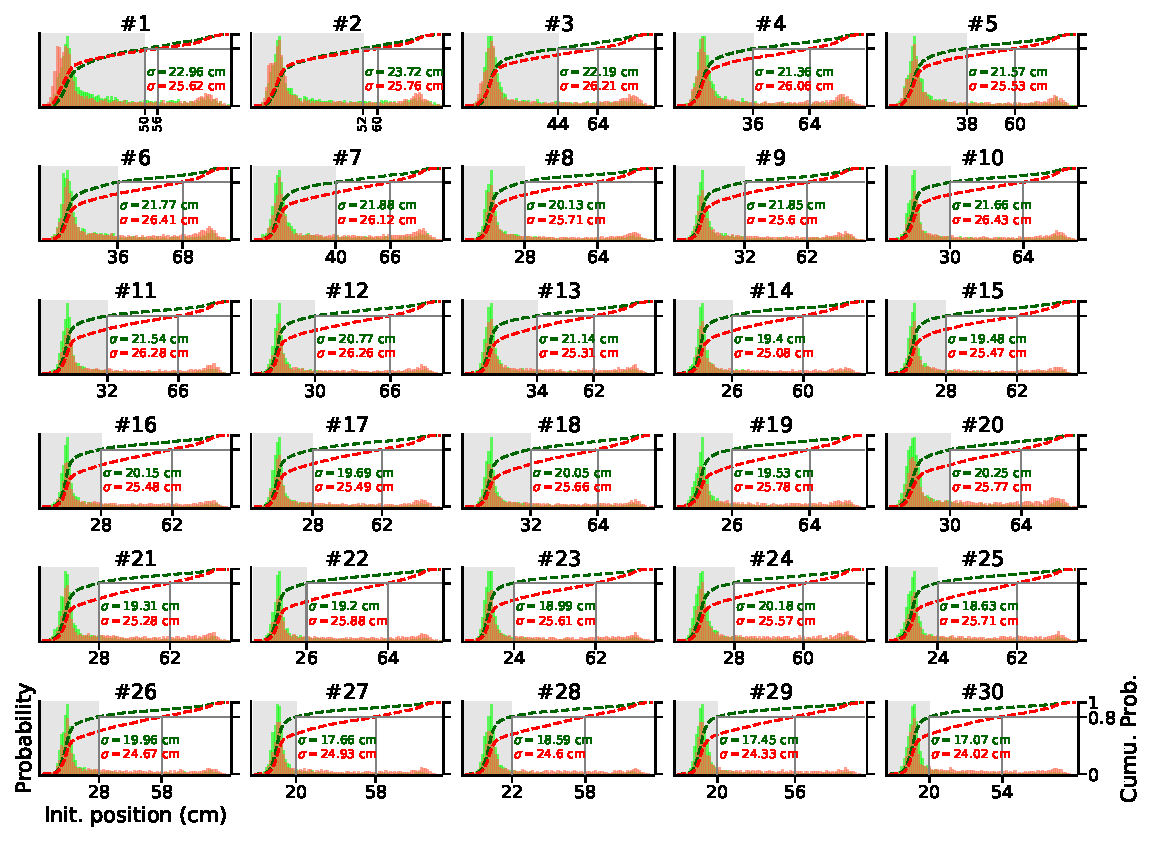
\includegraphics[width=\textwidth]{ch-appendicies/figures/InitPos.pdf}
    \caption[Initial Position Evolution]
    {\textbf{Initial position distributions for correct and error trials diverged progressively during training.}
    Similar to \Autoref{fig:time:CtrlTrd}{e}, each panel shows PDF of the initial position of the animals for correct (green) and error (red) trials, but plotted separately for each training session (\#1 to \#30).
    Dashed lines represent cumulative distribution functions (right y-axis).
    For each PDF, `$\sigma$' values denote the standard deviation.
    Each PDF included pooled data from all the animals trained in the control condition ($n=54$).
    }
    \label{fig:appendix:initPos}
  \end{center}
\end{figure}
\clearpage
\begin{figure}[!h]
  \begin{center}
    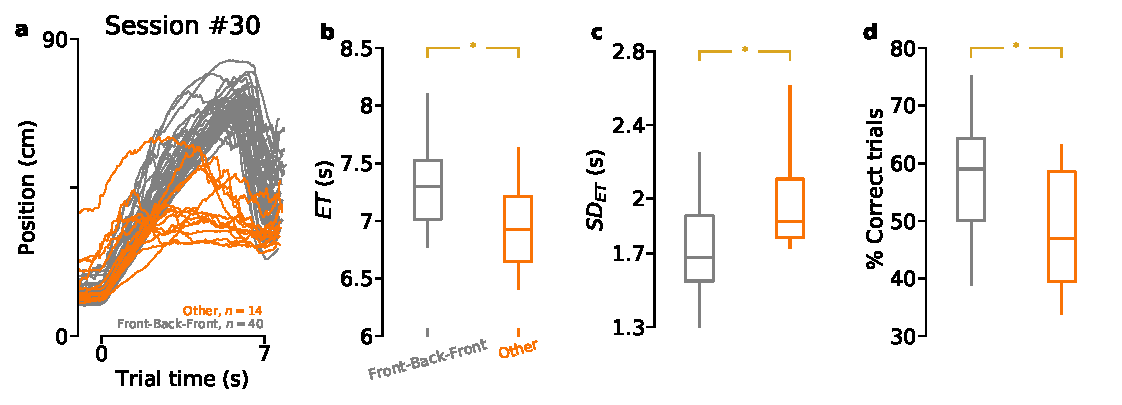
\includegraphics[scale=1]{ch-appendicies/figures/BadCtrl.pdf}
    \caption[Different Control Trajectory Groups]
    {\textbf{Task proficiency according to the type of trajectory performed by animals.}
    \textbf{a)}
    Same as \autoref{fig:time:CtrlTrd}, panel~c,~right, but the animals were divided in two groups according to whether they performed the front-back-front trajectory (gray) or not (other, orange).
    \textbf{b)}
    Entrance times($ET$s).
    $p=0.0066$ (permutation test).
    \textbf{c)}
    $SD$ of $ET$.
    $p=0.03$ (permutation test).
    \textbf{d)}
    Percentage of correct trials.
    $p=0.01$ (permutation test).
    For panels~b,~c,~d, same color code as in panel~a.
    Data from sessions \#~$\geq20$ were averaged for each animal.
    }
    \label{fig:appendix:BadCtrl}
  \end{center}
\end{figure} 

\clearpage
\begin{figure}[bt!]
  \begin{center}
    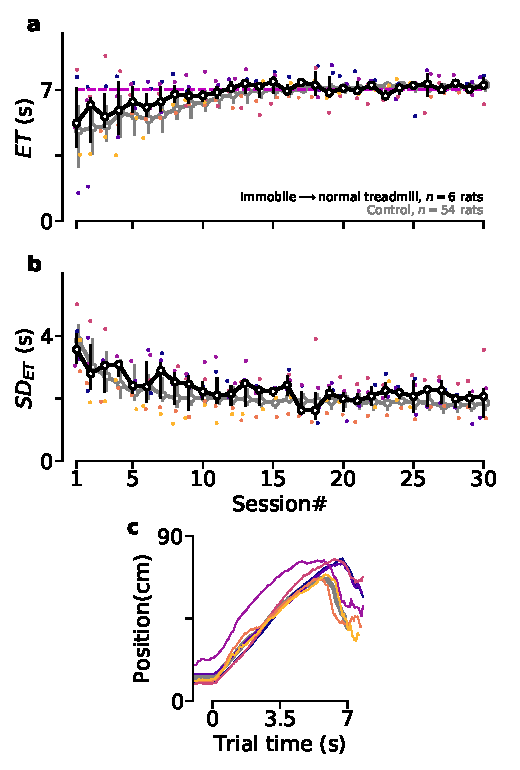
\includegraphics[scale=1]{ch-appendicies/figures/Imm2CtrlTrd.pdf}
    \caption[Immobile Animals Relearning the Task]
    {\textbf{Lack of temporal knowledge transfer across task protocols.}
    After extensive training on the immobile treadmill, animals were trained under normal conditions (GT$=7$~s, treadmill speed$=10$~cm/s).
    \textbf{a)}
    Median $ET$ across sessions under control condition.
    \textbf{b)}
    Similar to panel~a, for the standard deviation of entrance times ($SD_{ET}$).
    \textbf{c)}
    Median trajectory of the individual animals after relearning the task under the control condition.
    \textbf{a-c)}
    Individual animal color code is preserved in all panels.
    }
    \label{fig:appendix:Imm2Ctrl}
  \end{center}
\end{figure}
\clearpage
\begin{figure}[h!]
	\begin{center}
		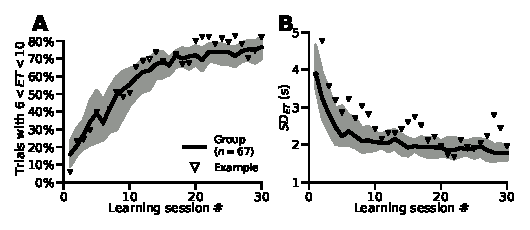
\includegraphics[scale=1]{ch-appendicies/figures/CorrectTrialCurve.pdf}
		\caption[Task Performance Improvement]
		{\textbf{Task performance improvement across sessions.}
		\textbf{A)}
		Percentage of trials in which animals entered the reward area close to the GT ($6~s<ET<10~s$), session-by-session.
		\textbf{B)}
		Session-by-session standard deviation of ET.
		Triangles show performance improvement for the example animal in \autoref{fig:lesion:task}.
		}
		\label{fig:appendix:CorrectTrialCurve}
	\end{center}
\end{figure}
\clearpage
\begin{figure}[bth!]
  \begin{center}
    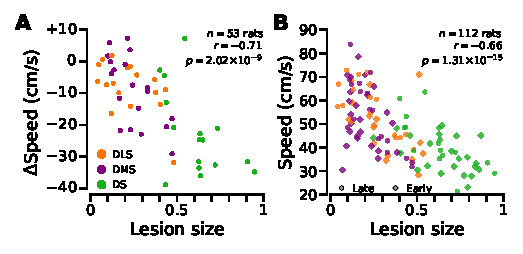
\includegraphics[scale=1]{ch-appendicies/figures/Speed.pdf}
    \caption[Speed-Lesion Size Correlation]
    {\textbf{The impact of the dS lesion on running speed correlates with lesion size.}
    \textbf{(A)} Average change in running speed (speed before lesion$-$speed after lesion) versus lesion size, for all the rats that received a striatal lesion after training (late lesion).
    Running speed was calculated when rats crossed the treadmill from its back region to the reward area.
    All the running speed values obtained across 5 consecutive sessions were averaged to obtain the average running speed before (last 5 sessions before lesion break) and after (sessions \#4 to \#9, relative to lesion break) lesion. 
    \textbf{(B)} Average running speed versus lesion size for all the animals that underwent surgical lesion of the dS.
    This dataset ($n=112$ animals) includes all the animals that underwent striatal lesion (DLS, DMS, DS) after extensive training (Late group, $n=53$, same animals as in panel A), and animals that underwent lesion before training (Early group, $n=59$ animals).
    Speed was computed as in A, except that average was done over session \#25 to \#30, relative to task training onset for the early lesion group.
    }
    \label{fig:appendix:spd}
  \end{center}
\end{figure}
\clearpage
\begin{figure}[h!]
	\begin{center}
		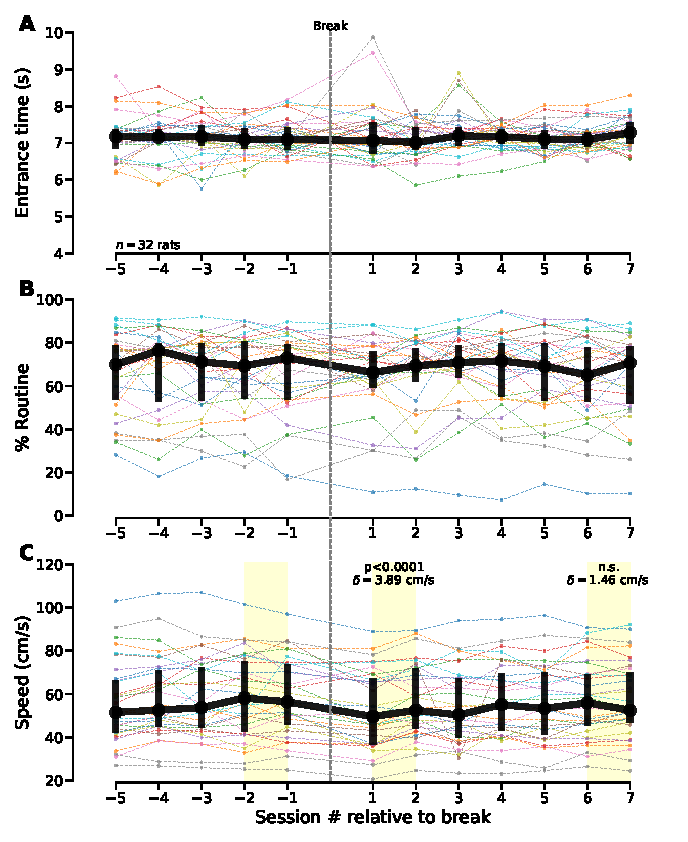
\includegraphics[scale=1]{ch-appendicies/figures/BreakEffect.pdf}
		\caption[Impact of a Two-week Break]
		{\textbf{Impact of two weeks of break on performance.}
		Task performance before and after a two week-long break in practice.
		Non-lesioned animals had stable performance before the two week-long break (same duration than lesion recovery period) in practice (\textit{A}: ET; \textit{B}: percentage of trials during which animals used the wait-and-run routine; \textit{C}: speed of the animals when they ran toward the reward area).
		A small but significant reduction in running speed was observed just after the break ($\delta$ denotes the effect size) that was restored after a few more training sessions.
		}
		\label{fig:appendix:break}
	\end{center}
\end{figure}
\clearpage
\begin{figure}[h!]
	\begin{center}
		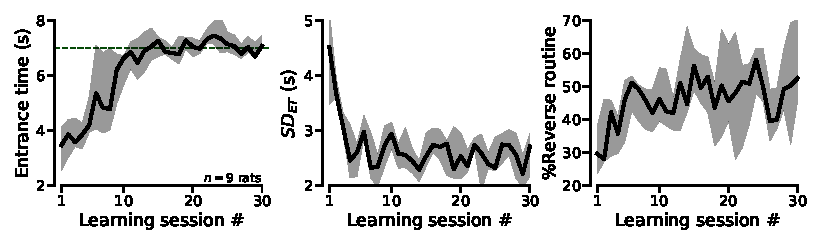
\includegraphics[scale=1]{ch-appendicies/figures/RevTrdLearning.pdf}
		\caption
		{\textbf{Performance improvement in the reverse treadmill task.}
		\textit{Left}: Entrance time across learning sessions.
		\textit{Middle}: Session-by-session standard deviation of ET.
		\textit{Right}: Percentage of trials during which animals used the run-and-wait (reverse) routine.
		}
		\label{fig:appendix:revLearn}
	\end{center}
\end{figure}
\clearpage
\begin{figure}[!h]
  \begin{center}
    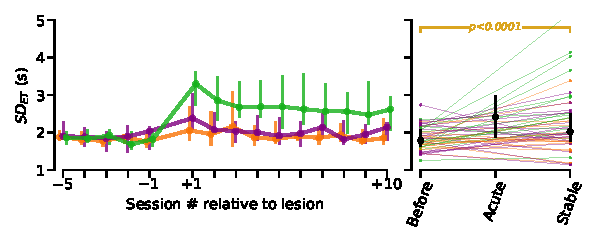
\includegraphics[scale=1]{ch-appendicies/figures/SDofET.pdf}
    \caption[Temporal Variability After Lesion]
    {\textbf{Temporal variability increased after striatal lesions.}
    \textit{Left}: session-by-session standard deviation of entrance times relative to lesion.
    colored traces show lesion groups (DLS, DMS, DS).
    \textit{Right}: statistical comparison of ET variability.
    Each line represents one animal.
    Same color-code as the left panel.
    }
    \label{fig:appendix:SdofET}
  \end{center}
\end{figure}
\clearpage
\begin{figure}[h!]
	\begin{center}
		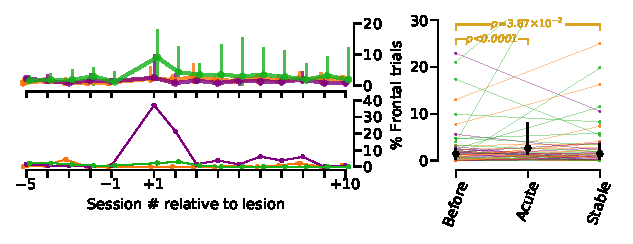
\includegraphics[scale=1]{ch-appendicies/figures/FrontalTrials.pdf}
		\caption[Frontal Trials After Striatal Lesion]
		{\textbf{Dorsal striatum lesions induced a transient increase in the percentage of trials during which animals remained close to the reward area.}
		\textit{Upper left}: Session-by-session percentage of trials in which animals remained close to the reward area (i.e., frontal trials).
		Group data for animals with DLS, DMS and DS lesion.
		Same color code for lesion types as in \autoref{fig:lesion:task}.
		\textit{Lower left}: Same as above, but for the illustrative animals, shown in \Autoref{fig:lesion:task}{E-G}.
		\textit{Right}: Group statistical comparisons before and after striatal lesion.
		There is an acute increase that is mostly restored after a few sessions.		
		}
		\label{fig:appendix:Frontal}
	\end{center}
\end{figure}


% % Make the bibliography single spaced
\singlespacing
\printbibliography[heading=bibintoc]
\printglossary[title=Acronyms, toctitle=Acronyms]

\end{document}